\documentclass[%
reprint,
superscriptaddress,
%groupedaddress,
%unsortedaddress,
%runinaddress,
%frontmatterverbose, 
%preprint,
%preprintnumbers,
%nofootinbib,
%nobibnotes,
%bibnotes,
 amsmath,amssymb,
 aps,
 prx,
%pra,
%prb,
%rmp,
%prstab,
%prstper,
longbibliography,
floatfix,
]{revtex4-2}
\usepackage{amsmath}
\usepackage{braket}
\usepackage{geometry}
\usepackage{amssymb}
\usepackage{amsfonts}
\usepackage{mathtools}
\usepackage{appendix}
\usepackage{url}
%\usepackage{floatrow}
\usepackage[utf8]{inputenc}
\usepackage{array}

\usepackage[dvipsnames]{xcolor}\usepackage[draft]{changes} %%%%---annotations are visible
\usepackage{color}   %May be necessary if you want to color links
\usepackage{hyperref}
\hypersetup{
    colorlinks=true, %set true if you want colored links
    linktoc=all,     %set to all if you want both sections and subsections linked
    linkcolor=blue,  %choose some color if you want links to stand out
}

\geometry{
 a4paper,
 total={170mm,257mm},
 left=20mm,
 top=20mm,
 }
 \usepackage{graphicx} 
%\usepackage{authblk}

\newcommand{\ER}[1]{{\color{purple}{{}[ER: #1]}}}
\newcommand{\sh}[1]{{\color{orange}{{}[SS: #1]}}}%for comments
\newcommand{\singh}[1]{{\color{orange}{{}#1}}}%for recommended edits
\newcommand{\gil}[1]{{\color{blue}{{}[GR: #1]}}}

\usepackage{orcidlink}

\begin{document}
\preprint{APS/123-QED}
\title{Impact of Josephson Junction Array modes on Fluxonium Readout}

\author{Shraddha Singh\orcidlink{0000-0002-4921-1410}}\thanks{Corresponding email: shraddha.singh@yale.edu}
\affiliation{Department of Applied Physics and Physics, Yale University, New Haven, Connecticut 06511, USA}
\affiliation{Yale Quantum Institute, Yale University, New Haven, Connecticut 06511, USA}
\affiliation{AWS Center for Quantum Computing, Pasadena, CA 91125, USA}
\author{Gil Refael}
\affiliation{AWS Center for Quantum Computing, Pasadena, CA 91125, USA}
\affiliation{Institute for Quantum Information and Matter,
California Institute of Technology, Pasadena, CA 91125}
\author{Aashish Clerk}
\affiliation{Pritzker School of Molecular Engineering, University of Chicago, Chicago, Illinois 60637, USA}
\affiliation{AWS Center for Quantum Computing, Pasadena, CA 91125, USA}
\author{Emma Rosenfeld}\thanks{Present address: Google Research}
\affiliation{AWS Center for Quantum Computing, Pasadena, CA 91125, USA}
\date{\today}%remove this eventually

\begin{abstract}
Fluxonium qubits, known for their high coherence and fast gates, are a promising candidate for superconducting architectures. High-fidelity measurement of these qubits is a crucial component in employing a fluxonium-based architecture for fault-tolerant quantum computing. We present an analysis of dispersive readout in fluxonium qubits, specifically considering the `parasitic' internal modes of a Josephson junction array (JJA) which constitutes the inductive shunt in the circuit. %Dispersive readout in superconducting circuits have already demonstrated measurements of fidelity $>0.99$. 
Measurement of superconducting circuits is currently limited by state transitions in the qubit, when increasing photons in the readout mode, also known as measurement-induced state transitions (MIST). 
Our analysis reveals that coupling to the parasitic modes of JJA introduces additional state transitions during fluxonium readout. Consequently, such parasitic-mode-assisted MIST processes, which we refer to as p-MIST, can lower the onset of MIST processes to as low as $\sim 10$ average photons in the readout mode, severely impacting the readout performance. We verify that, even upon neglecting nonlinearities in the JJA, a significant number of these parasitic transitions, mediated by the coupling of the parasitic mode to the qubit mode, occur at considerable rates. The residual population in the parasitic modes from p-MIST also causes significant dephasing of the resetted fluxonium qubit, after the readout pulse, limiting the performance of the qubit for future use. We extend our findings across various fluxonium circuits, analyzing the dependency of qubit-parasitic mode coupling on different circuit parameters. Our results underscore the substantial impact parasitic modes can have on the readout fidelity and the coherence of highly anharmonic superconducting circuits.
\end{abstract}
\maketitle
%\newpage
\section{Introduction}
%%%General fluxonium background%%%%
The fluxonium circuit, a Josephson junction shunted by an inductor and a capacitor, is a promising qubit due to its large anharmonicity, flexible parameters, and long lifetimes~\cite{high_coherence_2019, somoroff_millisecond_2023, single_cooper_pair, earnest_realization_2018}. Recent high-fidelity single-~\cite{zhang_universal_2021} and two-qubit~\cite{ding_high-fidelity_2023, zhang_tunable_2024} gate demonstrations show error probabilities of $\sim 10^{-4}$ and $\sim10^{-3}$, respectively, which likely can be improved further~\cite{nesterov_cnot_2022, nesterov_proposal_2021, dogan_two-Fluxonium_2023, rosenfeld_designing_2024, nguyen_blueprint_2022}. 
For this work, we assume that the inductive shunt in a fluxonium circuit constitutes a Josephson junction array (JJA)~\cite{masluk_microwave_2012, wang_achieving_2024} %, geometric inductors \cite{peruzzo_geometric_2021}, nanowires \cite{hazard_nanowire_2019}, and granular aluminum \cite{noauthor_granular_nodate, noauthor_granular_nodate-1}. Here we assume a typical Josephson junction array (JJA) inductance, 
due to its relatively low loss, large inductance, and small capacitance. The internal modes of the fluxonium circuit identify a qubit mode where the computational states reside, and several additional ``parasitic" modes, from the charge islands in the junction array ~\cite{ferguson2013symmetries}. 

%%%%%Measurement%%%%%%%%%%%%%
Typically, fluxonium qubit measurements are performed by dispersively coupling the circuit to a readout mode~\cite{{zhang_universal_2021}}. Dispersive readout, commonly used for its fast, single-shot capabilities, offers large signal-to-noise ratios and is expected to be quantum non demolition (QND)~\cite{blais2021circuit}. However, the fidelity and speed of this readout strategy has been limited by spurious transitions of the computational states to higher energy states~\cite{shillito2022dynamics,xiao2023diagrammatic,khezri2023measurement,cohen2023reminiscence,dumas2024unified,sank2016measurement}, often called Measurement-Induced State Transitions (MIST). Unlike the weakly anharmonic transmon, a fluxonium circuit is highly nonlinear~\cite{single_cooper_pair}, which increases the likelihood of MIST processes~\cite{nesterov2024measurement}. Additionally, any spurious modes, such as the JJA modes mentioned previously, box modes from chip packaging, or slot line modes in the chip geometry, may also play a role in MIST, as shown in Fig.~\ref{fig:demo}. However, a detailed analysis of MIST in the presence of such spurious modes during dispersive readout of a superconducting qubit is still pending.

%%%%This-Work (Our circuit and assumptions)%%%%%%%%%%%%%


\begin{figure}
    \centering
    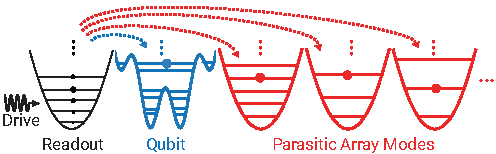
\includegraphics[width=\linewidth]{Figures/Demo.pdf}
    \caption{A parasitic effect where energy in a coherent state of the driven readout mode (black) excites extraneous parasitic modes (red) and the qubit mode (blue) simultaneously. %Schematic of qubit state transitions driven by a readout resonator with parasitic modes from a Josephson junction array (JJA). The cartoon circuit diagram is paired with energy profiles, showing energy in a coherent state of the driven readout mode (black) splitting into JJA parasitic modes (red), leaving enough energy for excitation in the qubit mode (blue).
    }
    \label{fig:demo}
\end{figure}

%\begin{figure}
    %\centering
    %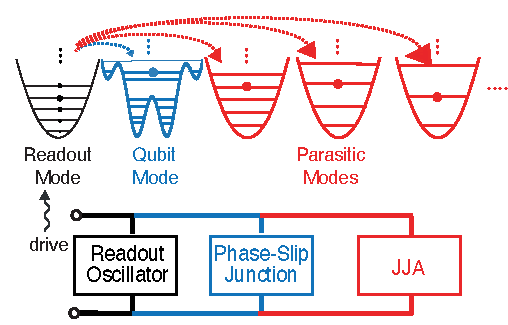
\includegraphics[width=\linewidth]{Fluxonium_Readout_manuscript/Figures/Demo_1.pdf}
%    \caption{Schematic of qubit state transitions driven by a readout oscillator (R) with parasitic modes from a Josephson junction array (JJA). The abstract circuit diagram is paired with energy profiles, showing energy in a coherent state of the driven readout mode (black) splitting into JJA parasitic modes (red), leaving enough energy for excitation in the qubit mode (blue).
%    }
%    \label{fig:demo1}
%\end{figure}
In this work, we analyze the state transitions during the dispersive readout of a fluxonium circuit, especially focusing on the effects that arise due to the parasitic modes of the JJA-fluxonium. Fig.~\ref{fig:meas_circuit} shows our measurement circuit for a heavy fluxonium circuit at the flux sweet spot  ($\varphi_\mathrm{ext}=0.5\Phi_0$), an experimentally-relevant choice for maximizing qubit coherence~\cite{somoroff_millisecond_2023,nguyen2019high,zhang_universal_2021,manucharyan2009fluxonium}; however, parasitic effects in the case of several circuit modifications are also discussed. While this figure shows a parallel circuit connection we have also analyzed different grounding configurations for single-point connection circuits in App.~\ref{app:alt_circuits}. In the main text, we mainly discuss the parallel circuit in Fig.~\ref{fig:meas_circuit} with circuit parameters inspired by the experiment in Ref.~\cite{zhang_universal_2021}. We analyze the population in the first three eigenstates in the qubit mode, to include experiments with a heavy fluxonium that use the first two levels ($01$) for computation and the second two levels ($12$) for measurement~\cite{zhang_universal_2021}. %The parasitic ground capacitance couples the various internal modes of a junction array. 
With our Hamiltonian derivations inspired from~\cite{viola2015collective}, we find that the coupling strength between the qubit mode and the parasitic modes can be $\sim 150 \ \mathrm{MHz}$, approximately ten-fold higher than the qubit-readout coupling strength. %Our calculations assume no self-nonlinearity in any mode except for the qubit mode. For the MIST analysis, we further simplify the system by considering only the parasitic mode with the strongest coupling to the qubit mode, the qubit mode itself, and the readout mode. 
\begin{figure}[htb]
%\begin{minipage}[b]{\linewidth}    
\centering    
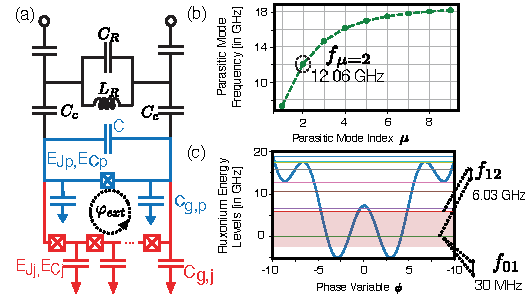
\includegraphics[width=\linewidth]{Figures/Meas_Circuit.pdf}
\caption{(a) Fluxonium readout circuit. The color scheme shows primary components that correspond to various modes, shown in Fig.~\ref{fig:demo}, when a JJA fluxonium circuit is connected to a readout resonator (R). The subscripts $p,j$ denote components of the phase-slip junction and the JJA, respectively. This circuit shows coupling capacitances ($C_c$), readout frequency parameters ($\omega_r/2\pi=1/\sqrt{L_{R}C_{R}}$), parasitic ground capacitances in JJA ($C_{g,j}$) and next to the phase-slip junction ($C_{g,p}$). The differential capacitance $C$ adjusts the charging energy of the qubit mode (see Table~\ref{tab:readout_params}). (b) Fluxonium mode energy levels in units of $h$, with the highlighted area showing the first three levels essential for certain readout schemes~\cite{zhang_universal_2021}. (c) Parasitic mode frequencies $\omega_\mu$. The lowest even mode $\mu = 2$ has the strongest coupling to the qubit (see Fig.~\ref{fig:coupling-strength}). 
}
\label{fig:meas_circuit}
\end{figure}
%\end{minipage}\hfill
\renewcommand{\arraystretch}{1.5} % Adjust the value as needed

\begin{table}[h]
\centering
\begin{tabular}{|c|c|c|c|c|c|c|c|c|c|}
    \hline
     $N$ & $\varphi_{ext}$ & $E_{J_p}$ & $E_{C_p}$ & $E_C$ & $E_{C_j}$ & $E_{J_j}$ & $E_{C_{g,j}}$ & $E_{C_{g,p}}$ & $E_c$ \\
    \hline
    $122$ & $0.5\Phi_0$ & $7.30$ & $0.74$ & $1.34$ & $0.74$ & $60$ & $194$ & $1.94$ & $19.40$ \\
    \hline
\end{tabular}
\caption{Circuit parameters for Fig.~\ref{fig:meas_circuit}(a) inspired by Ref.~\cite{zhang_universal_2021}. All energies are given in GHz. Here $\Phi_0=h/2e$ denotes the magnetic flux quantum. The capacitive energies $E_{C'}=\frac{19.4}{{C'}(fF)} \ \mathrm{GHz}$ are computed from the corresponding capacitances $C'$. See Table~\ref{tab:params} in App.~\ref{app:Hamiltonian} for the values of capacitances.}
\label{tab:circuit_params}
\end{table}
% The variables from left to right are the number of junctions in JJA, phase-slip junction energy, phase-slip capacitive energy, differential capacitance, JJA junction energy, JJA capacitive energy, ground capacitive energy in JJA, ground capacitive energy between JJA and phase-slip junction and coupling capacitive energy.
%%%%%%%%Our techniques and observations%%%%%%%%%%%%%

Treating the readout mode classically~\cite{cohen2023reminiscence,dumas2024unified}, we perform a Floquet simulation of this system and identify predominant MIST processes, shown in Fig.~\ref{fig:Floquet}. In particular, our simulation of the dispersive readout process identifies state transitions of the fluxonium mode under dispersive readout, which occur only in the presence of the coupling between the qubit mode and the parasitic mode. We term these phenomena Parasitic-Mode-Induced State Transition (p-MIST). At particular readout resonator frequencies, we find that the onset of p-MIST  can occur with only $\sim 10$ photons in the readout resonator, well within the desired power for high signal-to-noise ratios in dispersive readout~\cite{gusenkova2021quantum}.

%%%%%%Floquet%%%%%%
Our work identifies transition pathways not seen in previous Transmon-based MIST analyses, which occur because of the highly nonlinear nature of the fluxonium spectrum and the presence of strongly coupled parasitic modes. To understand the Floquet simulation results, we identify the processes that cause these transitions in Table.~\ref{tab:p-MIST} using energy-conservation processes which are supported by a perturbative estimation from Fermi's Golden (FG) rule calculations. We comment on the agreement with analytically calculated stark-shifted eigenenergies and FG rates of each transition in App.~\ref{app:Floquet-trans}. The total number of MIST processes increases by $~50\%$ in the presence of the parasitic mode that couples the strongest to the qubit mode. Examples of some interesting MIST processes are as follows. A higher energy fluxonium state ($\ket{2}$) may exchange population with a lower energy state ($\ket{0}$), through excitation exchange with the readout resonator in the presence of a parasitic mode. In our simulations, we also observe transitions between parity-conserving states which are impossible via a first-order process for $\varphi_\mathrm{ext}=0.5\Phi_0$. We also observe that two higher fluxonium states are hybridized into an equal superposition state when the drive frequency is resonant with their transition frequency; such hybridization allows for increased p-MIST processes. 

%%%%LZ+Dephasing%%%%%
We compute the rates of all p-MIST processes involving the $\ket{1}$ state, which is used for both measurement and computation, to justify that these transitions can be significant. The rates are computed independently from, (1) the Hamiltonian dynamics of the system, and (2) the quasi-energy gap obtained via the Floquet simulations in Landau-Zener probability calculations. We ringed up the drive towards the steady-state readout mode occupation of $\bar n_r=50$ to mimic dissipation in the readout resonator~\cite{dumas2024unified,cohen2023reminiscence}. Both methods indicate in perfect agreement that p-MIST processes triggered at $\bar n_r\sim 10$ can be significant at a ring-up rate of $\kappa_r=1 \ \mathrm{MHz}$. However, the two methods do not agree for $\kappa_r\ge 10$, indicating that the two-level Landau Zener physics does not capture the evolution of highly anharmonic fluxonium circuits. This observation needs further investigation and is a direction for future work.  The avoided crossings of such strong transitions can be correctly predicted using first-order perturbative calculations. In particular, these calculations show that p-MIST processes with a quasienergy gap larger than $\sim 0.5 \ \mathrm{MHz}$ at the avoided crossings occur with significant probability. 

Additionally, we show that the residual p-MIST population in the parasitic modes, which remains \textit{after} a readout pulse, begets significant dephasing of the qubit mode. Since these parasitic modes are long-lived~\cite{masluk_microwave_2012} and strongly coupled to the qubit mode, such residual population must be treated with care when designing the circuit. We numerically show that the dephasing error probability due to excited parasitic modes with finite internal quality factor is above the surface code error correction threshold for parameters used in the current experimental setups~\cite{masluk_microwave_2012,zhang_universal_2021,manucharyan2009fluxonium}. This effect indicates that, without proper care, the dephasing due to p-MIST could limit the performance of a fluxonium architecture.

\renewcommand{\arraystretch}{1.5} % Adjust the value as needed


\begin{table*}[tb]
    \centering
\begin{tabular}{|c|c|c|c|c|c|c|c|c|c|c|c|c|}
    \hline
    \textbf{Qubit ($\phi$) $\&$}&$\omega_{01}/2\pi$&$\omega_{12}/2\pi$ &$\tilde{E}^\phi_c$ &$g_{\phi r}/2\pi$&$\chi_{\phi r}(01)/2\pi$&$\chi_{\phi r}(12)/2\pi$&$\omega_r/2\pi$&$\kappa_r/2\pi$\\
    \cline{2-9}
\textbf{Readout ($r$)}&$30 \ \mathrm{MHz}$& $6.04 \ \mathrm{GHz}$ & $0.92 \ \mathrm{GHz}$& $25.50 \ \mathrm{MHz}$& $0.18 \ \mathrm{MHz}$&$0.98 \ \mathrm{MHz}$&$8.50 \ \mathrm{GHz}$&$1 \ \mathrm{MHz}$\\    
\hline\textbf{Parasitic-Mode} & \multicolumn{2}{c|}{} & $g_{\phi\mu}/2\pi$&$g_{\mu r}/2\pi$&$\chi_{\phi\mu}(01)/2\pi$&$\chi_{\phi\mu}(12)/2\pi$&$\omega_\mu/2\pi$&$Q_\mu$\\
    \cline{4-9}
\textbf{($\mu=2$)}&\multicolumn{2}{c|}{} &$157 \ \mathrm{MHz}$& $4.22 \ \mathrm{MHz}$& $-1.10 \ \mathrm{MHz}$& $5 \ \mathrm{MHz}$& $12.06 \ \mathrm{GHz}$&$10^{4}$\\    
\hline
\end{tabular}
\caption{Measurement parameters for qubit mode $\phi$, readout mode $r$ and closest even parasitic mode $\mu=2$.  All quantities are derived and computed analytically using circuit parameters listed in Table.~\ref{tab:circuit_params} (see App.~\ref{app:Hamiltonian} for details). \textbf{Qubit-Readout Parameters:} ($\omega_{ij}$) qubit $i\rightarrow j$ splitting frequency; ($\tilde{E}^\phi_c$) qubit charging energy; ($g_{\phi r}$) qubit-readout coupling; ($\chi_{\phi r}(ij)$) dispersive shift due to readout mode in the two-level $ij$ system; ($\omega_r$) readout mode frequency; ($\kappa_r$) decay rate of the readout resonator. \textbf{Parasitic-Mode Parameters:} ($g_{\phi \mu}$) qubit-parasitic coupling; ($g_{\mu r}$) parasitic-readout coupling; ($\chi_{\phi \mu}(ij)$) dispersive shift due to parasitic modes in the two-level $ij$ system; ($\omega_\mu$) mode frequency; and ($Q_\mu$) internal quality factor inspired by~\cite{masluk_microwave_2012}.}   \label{tab:readout_params}
\end{table*}

%%Sec 4%%%%
Finally, we generalize our results to several circuit modifications by analyzing the sensitivity of the parasitic mode-qubit coupling strength for different readout frequencies, parasitic mode frequencies, qubit mode frequencies, ground capacitances, and number of junctions in the array. First, we show that these effects are mediated strictly by the coupling between the qubit mode and the parasitic mode. We also explore lower readout frequencies in Fig.~\ref{fig:Flo_low} and show that increased p-MIST processes can be introduced if the parasitic frequency is an integer multiple of the drive frequency. In addition, we simulated a $\sim 300 \ \mathrm{MHz}$ circuit with larger parasitic mode frequencies, inspired by the experiment in Ref.~\cite{ding_high-fidelity_2023}. We find that for comparable frequencies and coupling strengths, this circuit shows a much lower number of MIST processes, an observation that needs further investigation beyond the scope of this work. However, even in this case, half the number of transitions (one out of two) are p-MIST for similar coupling strengths. While our analysis does not demonstrate an exhaustive study over the entire parameter space, it shows that the parasitic modes of a junction array introduce additional constraints on the circuit design of high-coherence fluxonium qubits.


%%%%%structure%%%%%%
The rest of the article is structured as follows. Sec.~\ref{sec:Fluxonium} details the readout circuit and its strong parasitic coupling under a linear JJA approximation. Through this assumption, our work presents the lower bound on the effects of JJA parasitic modes on the readout of a fluxonium circuit. Sec.~\ref{sec:MIST} covers readout dynamics, including MIST processes and dephasing from parasitic modes. Sec.~\ref{sec:expressions} analyzes the effects of coupling strengths on p-MIST, and investigates different ranges of readout frequencies and parasitic mode frequencies using an energy-conservation picture. Finally, in Sec.~\ref{sec:conclusion} we discuss directions for future work towards our analysis.

\section{Fluxonium Readout Circuit}\label{sec:Fluxonium}


%%%%Fluxonium circuit%%%%%%%%%%%%%%%%%%%%%%
We consider a JJA-fluxonium circuit dispersively coupled to a readout mode as shown in Fig.~\ref{fig:meas_circuit}. The parameters for circuit design used in our work, listed in Table~\ref{tab:circuit_params}, are motivated by recent experiments~\cite{zhang_tunable_2024,zhang_universal_2021}. We focus on the fluxonium circuit at the ``sweet spot" for maximal qubit coherence times. This choice is also expected to reduce the number of allowed transitions in the circuit, as transitions between parity-conserving states via first-order processes are forbidden in this case. Here, the qubit frequency ($\omega_{01}/2\pi$) is $\sim 30 \ \mathrm{MHz}$ and the plasmon frequency ($\omega_{12}/2\pi$) is $\sim 6 \ \mathrm{GHz}$, in this ``heavy" fluxonium regime (see Table~\ref{tab:readout_params} for a full list of readout parameters). The dispersive shift on the qubit computational states due to the readout resonator is not sufficiently strong for high signal-to-noise ratio, at $\chi_{01} \sim 0.2 \ \mathrm{MHz}$; in practice, higher excited states of the fluxonium qubit mode may be populated intentionally for improved readout fidelity \cite{zhang_universal_2021}. Thus, to also capture effects from measurement schemes that use higher levels ($1,2$), we consider the population in the lowest three states of the qubit mode. 

%%%%%%%%%JJA+assumptions%%%%%%%%%%%%%%%%
Our work specifically investigates the role of the JJA, which comprises the inductive shunt of the fluxonium. The array comprises $N+1$ junctions and $N$ ground capacitances due to the JJA ($C_{g_n}$)~\cite{manucharyan2009fluxonium}. We assume an ordered array with identical junctions and parasitic ground capacitances between these junctions ($C_{g_1}=..=C_{g_{N-1}}=C_{g,j}$). Two additional identical ground capacitances near the phase-slip junctions may have different values, with $C_{g_0}=C_{g_N}=C_{g,p}\neq C_{g, j}$. The JJA fluxonium circuit has $N$ internal degrees of freedom~\cite{ferguson2013symmetries,viola2015collective}: one qubit mode ($\phi$) and $N-1$ parasitic modes ($\mu$), where $\mu$ ranges between $1,...,N-1$. These  modes are coupled via the ground capacitances. 
% notation
In our notation, we label the readout mode as $r$. The charge and flux quadratures of the qubit mode are denoted by $\hat N_\phi$ and $\hat \phi$ where $[\hat \phi,\hat N_\phi]=\frac{i\hbar}{2}$. We simplify the problem by treating all but the qubit mode as harmonic oscillators as assumed in previous works~\cite{ferguson2013symmetries,viola2015collective,dumas2024unified}. This assumption will lower bound the effects of JJA parasitic modes on qubit performance for driven fluxonium circuits. We denote the photon loss and gain operators of the linear modes $r,\mu$ using $\hat a_r,\hat a_\mu$ and $\hat a_r^\dagger,\hat a_\mu^\dagger$, respectively. 

In units of $\hbar=1$, the Hamiltonian of an undriven fluxonium measurement circuit has the form (see App.~\ref{app:alt_circuits} for derivation)

\begin{equation}
   \hat H =\hat{H}_\phi + \hat{H}_\mu + \hat{H}_r + \hat{H}_{int},\label{Hamiltonian_total}
\end{equation}
where the qubit Hamiltonian $\hat{H}_\phi$ (with JJA inductive energy $E_L=E_{J_j}/N$) is 
\begin{equation}
% \hat{H}_\phi = 8\pi\tilde{E}^\phi_c \hat N_\phi^2+2\pi E_{J_p}\cos{\hat\phi}+\pi E_L\hat \phi^2,
\hat{H}_\phi / 2\pi = 4\tilde{E}^\phi_c \hat N_\phi^2+ E_{J_p}\cos{\hat\phi}+E_L\hat \phi^2 /2,
\end{equation}
the junction array and readout Hamiltonians are $\hat{H}_\mu = \sum_{\mu}\omega_\mu \hat a_\mu^\dagger \hat a_\mu$ and $\hat{H}_r = \omega_r \hat a_r^\dagger \hat a_r$, respectively. The qubit charging energy deviates from the target value of $E_c^{\phi}=1 \ \mathrm{GHz}$ due to parasitic capacitance. The coupling between the three modes is described by the interaction Hamiltonian
\begin{align}\label{eq:int_hamiltonian}
\hat{H}_{int} = g_{\phi r} \frac{\hat N_\phi}{{N_{\phi,ZPF}}} (\hat a_r-\hat a_r^\dagger)\nonumber \\ -\sum_{\mu} g_{\phi\mu} \frac{\hat N_\phi}{{N_{\phi,ZPF}}} (\hat a_\mu-\hat a_\mu^\dagger) \nonumber \\- \sum_{\mu} g_{\mu r} (\hat a_r-\hat a_r^\dagger)(\hat a_\mu-\hat a_\mu^\dagger).
\end{align}
where the zero-point fluctuation value is $N_{\phi,ZPF}=1.4$. Values for all remaining variables used in the above equations are given in Table.~\ref{tab:readout_params}.


%%%%%choosing the lowest even mode %%%%%
 Our coupling strengths follow the same relative behaviour as observed in Ref.~\cite{viola2015collective}, but with a different set of parameters as chosen here. We find that the lowest-frequency even parasitic mode $\mu=2$ has the strongest coupling to the qubit mode (see Fig.~\ref{fig:coupling-strength} in App.~\ref{app:Hamiltonian}); parasitic parameters are quoted in Table~\ref{tab:circuit_params}. Ref.~\cite{viola2015collective} shows that the symmetry of the parallel circuit in Fig.~\ref{fig:meas_circuit} prevents coupling between odd parasitic modes (including $\mu=1$) and other circuit modes. We extend this result to two additional circuits, with different ground circuit configurations, showing qualitatively consistent conclusions across all in App.~\ref{app:alt_circuits}. The circuits yield the same Hamiltonian when the differential capacitance $C$ and coupling capacitance $C_c$ are altered such that qubit frequency and qubit-readout coupling are same across all three circuits (see Table~\ref{tab:parasitic_params} in App.~\ref{app:alt_circuits}). With these observations, in the rest of this work, we will use the parallel circuit from Fig.~\ref{fig:meas_circuit} using parameters given by Tables~\ref{tab:circuit_params},~\ref{tab:readout_params} in Eq.~\ref{Hamiltonian_total} with only the qubit $(\phi)$, the strongest coupled parasitic mode $(\mu=2)$ and the readout resonator $(r)$. For details on other parasitic modes and their circuit parameters, see Apps.~\ref{app:Hamiltonian}. 
 
As reported in Table~\ref{tab:circuit_params}, the qubit couples roughly six times more strongly to the parasitic mode at $\mu=2$ than it does to the readout $r$~\footnote{In fact, the first four even parasitic modes with coupling strengths within a factor of $10$ of $g_{\phi r}$. See Fig.~\ref{fig:coupling-strength} in App.~\ref{app:Hamiltonian}}. As we highlight in the next section, such strong couplings can lead to measurement-induced state transitions assisted by parasitic modes, termed ``p-MIST". Note that this coupling is also responsible for indirectly coupling the readout with the parasitic modes since $g_{\mu r}\propto g_{\phi\mu}$. 

\section{Parasitic-mode-Assisted MIST: p-MIST}\label{sec:MIST}

 In this section, we will analyze how the presence of a parasitic mode ($\mu=2$) affects the dynamics of a driven fluxonium circuit in a readout context. To simulate the linear drive on the readout resonator, we add a drive term $V_d=i\xi (\hat a_r-\hat a_r^\dagger)\cos{\omega_d t}$ to the system Hamiltonian in Eq.~\ref{Hamiltonian_total}. If we consider the fluxonium qubit mode, parasitic modes, and readout resonator, numerical analyses of several excitations in the circuit would require a prohibitively large Hilbert space. For example, the highly nonlinear nature of the fluxonium qubit spectrum results in a minimum Hilbert space dimension of at least $\sim 20$ for an accuracy of \singh{$1 \ \mathrm{MHz}$~\cite{??}}, while we expect to drive many photons in the readout cavity. To truncate our Hilbert space to feasible dimensions for numerical simulations, here we only include a single parasitic mode $\mu=2$ (as previously justified in Sec.~\ref{sec:Fluxonium}), and we replace the readout mode with a classical drive term~\cite{cohen2023reminiscence,dumas2024unified,xiao2023diagrammatic} using the derivation in App.~\ref{app:MIST}. Under this semi-classical approximation, we give the driven circuit Hamiltonian with only two modes, $\phi$ and $\mu=2$
\begin{align}
  \hat H_{s.c.}(\bar n_r)=\hat H_0+\hat V_{s.c.}(\bar n_r)  \label{eq:drive_Ham}
\end{align}
 which includes the parent or bare Hamiltonian,
\begin{align}
H_0=\hat H_\phi+\hat H_{\mu}-\frac{g_{\phi\mu}}{N_{\phi,ZPF}} \hat N_\phi (\hat a_{\mu}-\hat a_{\mu}^\dagger) \label{eq:bare_ham} 
\end{align}
and the modified drive term $V_{s.c.}$,
\begin{align}
    \hat V_\textrm{s.c.}(\bar n_r)&=\frac{\xi_{\phi r}(\bar n_r)}{N_{ZPF,\phi}} \hat N_\phi\cos{\omega_d t}+\xi_{\mu r}(\bar n_r) \hat N_\mu\cos{\omega_d t}\label{eq:drive},
\end{align}
where $\xi_{\mu(\phi) r}(\bar n_r)=2g_{\mu(\phi) r}\sqrt{\bar n_r}$, and $\bar n_r$ denotes average readout photons, respectively. We shall call the quantities $\xi_{\phi r/\mu r}$ qubit and parasitic drive strengths, respectively. Note that a similar semi-classical approximation could have been carried out to remove the parasitic mode from the picture, however, the quantum fluctuations cannot be ignored in this case since the parasitic modes are not expected to be highly populated in readout experiments, and also, doing this will not capture the physics we are interested in. 


Our primary task is to analyze p-MIST processes which introduce simultaneous transitions in the parasitic mode and the qubit mode. To identify the state transitions in the driven circuit, we first examine the eigenspace of the bare Hamiltonian $H_0$ in Eq.~\ref{eq:bare_ham}. Commonly, for the analysis of a fluxonium circuit, the basis $\ket{k}_{\phi} \otimes \ket{n}_{\mu}$ is used, where the parasitic mode $\mu$ is mostly ignored~\cite{nesterov2024measurement}. We label the hybridized eigenstates of $H_{\textrm{0}}$ as  $\ket{\tilde{k}, \tilde{n}}$ to indicate the states, it has maximum overlap with, in the disjoint Hilbert space $\ket{k}_\phi\otimes\ket{n}_\mu$. This labeling will help us better understand the effects of p-MIST on the qubit subspace.


Next, we perform a Floquet simulation of the driven circuit to identify the state transitions in the system. We simulate the system dynamics for a range of readout resonator frequencies, $\omega_d$, and ring up the various drive strengths $\xi_{\mu/\phi}$ to emulate the addition of photons in the readout resonator. We find that the presence of the parasitic mode $\mu=2$ significantly increases the number of MIST processes in the system. We analyze the processes that cause these transitions and quantify their rates using perturbative approaches and Landau Zener probability calculations~\cite{ikeda2022floquet}. We also show that the residual population in the parasitic modes, after a readout pulse, can lead to significant dephasing of the resetted qubit mode, limiting the performance of the qubit for any future use.

\subsection{Floquet Simulations} 
\begin{figure}[!htb]
    \centering
    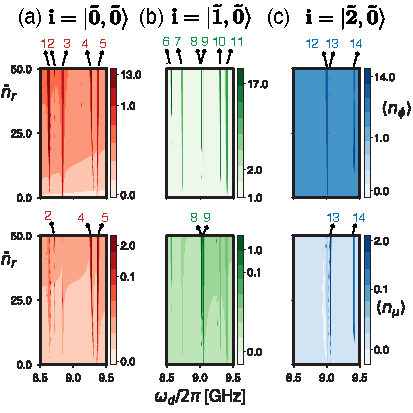
\includegraphics[width=0.5\textwidth]{Figures/Floquet_min.pdf}
    \caption{p-MIST processes in Floquet Simulations. Columns show results for branch analysis starting in the dressed hybridized eigenstate $i=\ket{\tilde{k},\tilde{0}}$, with maximum overlap to the un-hybridized states $\ket{k}_\phi\otimes\ket{0}_{\mu=2}$. \textbf{Top row:} Average fluxonium excitation $\langle n_\phi\rangle $. \textbf{Bottom row:} Average excitation of the first-even parasitic mode $\mu=2$ $\langle n_\mu\rangle$. The plots are shown in log scale as a visual aid for all marked transitions, explicitly listed in Table~\ref{tab:p-MIST}. See Figs.~\ref{fig:Trans0}-\ref{fig:Trans2} of App.~\ref{app:Floquet-trans} for quasienergies.}
    \label{fig:Floquet}
\end{figure}
\begin{table*}[!bth]
    \centering
    \begin{tabular}{w{c}{2.0cm}w{c}{3.0cm}w{c}{2.0cm}w{c}{2.0cm}w{c}{2.5cm}w{c}{1.5cm}w{c}{2.5cm}}
\hline
\shortstack{\\\textbf{Transition }\\\textbf{No.}\\\textbf{ (see Fig.~\ref{fig:Floquet})}} &\shortstack{\\\textbf{Fluxonium}\\\textbf{MIST}\\\textbf{Process}} &\shortstack{\\\textbf{Threshold}\\\textbf{Drive}\\\textbf{Photon ($\bar n_r$)}}& \shortstack{\\\textbf{Drive}\\\textbf{Frequency}\\($\omega_d$)}& \shortstack{\\\textbf{Quasienergy}\\\textbf{Gap}\\($\Delta_{ac}$)}& \textbf{p-MIST}&\shortstack{\textbf{Drive Photons}\\\textbf{Absorbed}\\\textbf{(see Fig.~\ref{fig:trans_prof})}}\\
\hline
\rule{0pt}{4ex}$1.$&$\color{BrickRed}{\ket{\tilde{0},\tilde{0}}}$$\xleftrightarrow []{\hspace{1em}}\ket{\tilde{13},\tilde{0}}$&$13$ &$8.64 \ \mathrm{GHz}$&$0.90 \ \mathrm{MHz}$&$\times$ & $3$\\
%\hline
$2.$&$\color{BrickRed}{\ket{\tilde{0},\tilde{0}}}$$\xleftrightarrow[]{\hspace{1em}}\ket{\tilde{4},\tilde{2}}^*$ &$48$&$8.71 \ \mathrm{GHz}$&$0.06 \ \mathrm{MHz}$&$\color{BrickRed}{\checkmark}$ & $4$\\
%\hline
$3.$&$\color{BrickRed}{\ket{\tilde{0},\tilde{0}}}$$\xleftrightarrow[]{\hspace{1em}}\ket{\tilde{8},\tilde{0}}$ &$\sim 0$&$8.84 \ \mathrm{GHz}$&$-$&$\times$ &$2$\\
%\hline
$4.$&$\color{BrickRed}{\ket{\tilde{0},\tilde{0}}}$$\xleftrightarrow[]{\hspace{1em}}\ket{\tilde{6},\tilde{1}}^*$&$46$&$9.25 \ \mathrm{GHz}$&$1.63 \ \mathrm{MHz}$&$\color{BrickRed}{\checkmark}$ &$2$\\
$5.$&$\color{BrickRed}{\ket{\tilde{0},\tilde{0}}}$$\xleftrightarrow[]{\hspace{1em}}\ket{\tilde{3},\tilde{1}}$ &$12$&$9.36 \ \mathrm{GHz}$&$0.56 \ \mathrm{MHz}$&$\color{BrickRed}{\checkmark}$ &$2$\\
%\hline
$6.$&$\color{ForestGreen}{\ket{\tilde{1},\tilde{0}}}$$\xleftrightarrow[]{\hspace{1em}}\ket{\tilde{17},\tilde{0}}$ &$32$&$8.56 \ \mathrm{GHz}$&$0.25 \ \mathrm{MHz}$&$\times$ & $4$\\
%\hline
$7.$&$\color{ForestGreen}{\ket{\tilde{1},\tilde{0}}}$$\xleftrightarrow[]{\hspace{1em}}\ket{\tilde{7},\tilde{0}}$ &$4$&$8.73 \ \mathrm{GHz}$&$0.74 \ \mathrm{MHz}$&$\times$ & $2$\\
%\hline
$8.$&$\color{ForestGreen}{\ket{\tilde{1},\tilde{0}}}$$\xleftrightarrow[]{\hspace{1em}}\ket{\tilde{12},\tilde{1}}$&$19$&$9.02 \ \mathrm{GHz}$&$0.12 \ \mathrm{MHz}$&$\color{ForestGreen}{\checkmark}$ & $4$\\
%\hline
$9.$&$\color{ForestGreen}{\ket{\tilde{1},\tilde{0}}}$$\xleftrightarrow[]{\hspace{1em}}\ket{\tilde{2},\tilde{1}}$  &$11$&$9.05 \ \mathrm{GHz}$&$0.66 \ \mathrm{MHz}$&$\color{ForestGreen}{\checkmark}$ & $2$\\
%\hline
$10.$&$\color{ForestGreen}{\ket{\tilde{1},\tilde{0}}}$$\xleftrightarrow[]{\hspace{1em}}\ket{\tilde{14},\tilde{0}}$ &$7$&$9.31 \ \mathrm{GHz}$&$0.50 \ \mathrm{MHz}$&$\times$ & $3$\\
%\hline
$11.$&$\color{ForestGreen}{\ket{\tilde{1},\tilde{0}}}$$\xleftrightarrow[]{\hspace{1em}}\ket{\tilde{9},\tilde{0}}$ &$2$&$9.41 \ \mathrm{GHz}$&$1.19 \ \mathrm{MHz}$&$\times$ &$2$\\
%\hline
$12.$&$\color{RoyalBlue}{\ket{\tilde{2},\tilde{0}}}$$\xleftrightarrow[]{\hspace{1em}} \ket{\tilde{12},\tilde{0}}$ &$1$&$9.00 \ \mathrm{GHz}$&$0.73 \ \mathrm{MHz}$&$\times$ & $2$\\
%\hline
$13.$&$\color{RoyalBlue}{\ket{\tilde{2},\tilde{0}}}$$\xleftrightarrow[]{\hspace{1em}}\ket{\tilde{0},\tilde{2}}$&$38$&$9.06 \ \mathrm{GHz}$&$0.53 \ \mathrm{MHz}$&$\color{RoyalBlue}{\checkmark}$ & $2$\\
%\hline
$14.$&$\color{RoyalBlue}{\ket{\tilde{2},\tilde{0}}}$$\xleftrightarrow[]{\hspace{1em}}\ket{\tilde{5},\tilde{1}}^*$ &$41$&$9.41 \ \mathrm{GHz}$&$2.71 \ \mathrm{MHz}$&$\color{RoyalBlue}{\checkmark}$ & $2$\\
\hline
\end{tabular}
\caption{Measurement-induced-state-transition (MIST) observed in Fig.~\ref{fig:Floquet}. Column $1$ lists the numbering used to mark the transitions in Fig.~\ref{fig:Floquet}. Here $\ket{\tilde{i},\tilde{j}}$ indicates the hybridized eigenstates of $H_0$ (see Eq.~\ref{eq:bare_ham}) which have the maximum overlap with the state $\ket{i}_\phi\otimes \ket{j}_{\mu=2}$ in the disjoint Hilbert space of qubit mode ($\phi$) and parasitic mode ($\mu=2$). Column $2$ lists the MIST processes that start  at the lowest average readout photon number $\bar n_r$ given by column $3$. In some cases, we use $\bar n_r\sim 0$ to indicate that the drive frequency is exactly resonant with the transition frequency. A `$^*$'-marked state indicates hybridization at lower $\bar n_r$ due to preceding transitions~\footnote{$\ket{\tilde{4},\tilde{2}}^*:\ket{\tilde{4},\tilde{2}}\xleftrightarrow[]{\hspace{1em}}\ket{\tilde{14},\tilde{2}}$ at $\bar n_r=5, \omega_d=8.71 \ \mathrm{GHz}$ with $\Delta_{ac}=4.0 \ \mathrm{MHz}$ absorbs $2$ drive photons\\$\ket{\tilde{6},\tilde{1}}^*:\ket{\tilde{6},\tilde{1}}\xleftrightarrow[]{\hspace{1em}}\ket{\tilde{3},\tilde{1}}$ at $\bar n_r\sim 0, \omega_d=9.25 \ \mathrm{GHz}$\\$\ket{\tilde{5},\tilde{1}}^*:\ket{\tilde{5},\tilde{1}}\xleftrightarrow[]{\hspace{1em}} \ket{\tilde{17},\tilde{0}}$ at $\bar n_r=14, \omega_d=9.41 \ \mathrm{GHz}$ with $\Delta_{ac}=4.2 \ \mathrm{MHz}$ absorbs $1$ drive photon}. Column $4$ yields the quasienergy gap at the avoided crossing labeled as $\Delta_{ac}$. Column $5$ represents the drive frequency $\omega_d$ at which these transitions occur. Column $6$ indicates if the process cannot occur without the parasitic mode, denoted as p-MIST. Column $7$ indicates the number of drive photons ($\#$) involved in the energy-conserving process, illustrated in Fig.~\ref{fig:trans_prof}. which is responsible for these transitions. We give a comparison of Fermi's golden rule rates and quasienergies for these processes in App.~\ref{app:Floquet-trans}.
}
    \label{tab:p-MIST}
\end{table*}

Our first numerical analysis uses Floquet simulation of the Hamiltonian $H_{s.c.}$ (see Eqs.~\ref{eq:drive_Ham}) while varying $\bar n_r$ as the Floquet parameter, for various drive frequencies $\omega_d$. To reduce the numerical complexity, we only focus on transitions involving the lowest $20$ levels in the qubit subspace $\phi$ and $2$ levels in the harmonic oscillator mode $\mu=2$ with a maximum of $50$ photons in the readout resonator. In App.~\ref{app:numerics} we discuss the truncation~\footnote{We show that our results hold when simulated with $30$ levels in the qubit mode and $10$ levels in the parasitic mode} used to obtain our results. %\sh{Yet to put Truncation+Derivation in Appendix}. 
As indicated before, we will study transitions from states $\ket{i} =\ket{\tilde{\phi}, \tilde{\mu}}$ where $\phi\in\{0,1,2\}$ and $\mu=0$. With $\omega_\mu=12.06 \ \mathrm{GHz}$, the analysis in this section will consider the regime of negative detuning where, $\omega_{\mu=2}>\omega_d=\omega_r>>\omega_q$, and can be replicated for any other parasitic mode. Note that we also analyze the effects of an alternative circuit with $\omega_{\mu=2}\sim 16 \ \mathrm{GHz}$ and $\omega_\phi\sim 300 \ \mathrm{MHz}$ in Sec.~\ref{sec:expressions}.


Inspired by~\cite{dumas2024unified,cohen2023reminiscence}, we extract p-MIST processes by tracking a hybridized fluxonium eigenstate in a Floquet simulation while ringing up the drive strengths, a method known as \emph{branch analysis}. Our drive ring-up emulates the addition of a single readout photon by incrementing $\bar n_r$ for each tracking step at $t=0$. The simulation begins in an eigenstate $\ket{i}$ of the bare Hamiltonian $\hat{H}_0$ (see Eq.~\ref{eq:bare_ham}). This state is the same as the dressed eigenstate of the driven circuit Hamiltonian $H_{s.c.}$ (see Eq.~\ref{eq:drive_Ham}) at $\bar n_r=0$, $\ket{i}_{\bar n_r=0}$. Next, we compute the dressed eigenstates of the modified Hamiltonian $\hat{H}_{s.c.}$ at $\bar n_r=1$, $\{\ket{m}_{\bar n_r=1}\}$, corresponding to a single photon increase in the readout resonator. We then track the eigenstate $\ket{i}_{\bar n_r=1}$ in this new eigenspace that has maximum overlap with $\ket{i}_{\bar n_r=0}$, identifying it as the new eigenstate associated with the branch of $\ket{i}$. This process is repeated with the increment $\Delta \bar n_r=1$, such that at each tracking step $t_k$, a new state is chosen from the Floquet eigenspace of the modified Hamiltonian, yielding the branch
\begin{align}
\ket{i_{\bar n_r=k}}:\max_{m}|\braket{i_{\bar n_r=k-1}|{m}_{\bar n_r=k}}|^2.   
\end{align}
Our method is different from Ref.~\cite{dumas2024unified,cohen2023reminiscence} in that we perform the branch analysis of the modified Hamiltonians $H_{s.c.}(\bar n_r)$ at a fixed time $t=0$ while linearly varying $\bar n_r$. In the time evolution picture, the drive powers $|\xi_{\phi r}|^2,|\xi_{\mu r}|^2 \propto \bar n_r$ are increasing linearly in time as $\bar n_r= \kappa t/T$, where $\kappa \Delta t=T$. For each $\ket{i_{\bar n_r=m}}$ tracked in the branch, we compute:
\begin{enumerate}
    \item the average expectation values of $\hat n_\phi=\sum_k k\ket{k}_\phi\bra{k}_\phi$ where $k$ is the index for the bare fluxonium eigenstates $\ket{k}_\phi$,
    \item the expectation value of $\hat n_\mu=\hat a_{\mu}^\dagger \hat a_{\mu}$, the number operator of the harmonic oscillator defined by the parasitic mode $\mu=2$, and 
    \item the quasi-energy spectrum $E_i\mod \omega_d$.
\end{enumerate}

Fig.~\ref{fig:Floquet} illustrates our main result, showing p-MIST for initial states that have maximum overlap with states $\ket{0}_\phi$, $\ket{1}_\phi$ and $\ket{2}_\phi$ in the fluxonium subspace and the ground state $\ket{0}_{\mu=2}$ in the parasitic subspace. We focus on readout drive frequencies in the experimentally motivated target range $8.5 - 9.5 \ \mathrm{GHz}$~\footnote{a relatively high-frequency choice, to reduce thermal, photon shot-noise induced dephasing in the qubit compared to lower-frequency bands} while other ranges of readout frequencies are also discussed in Sec.~\ref{sec:expressions}. The y-axes of the various plots show average readout photons $\bar n_r$ which is directly proportional to the variation in drive powers $|\xi_{\phi r}|^2,|\xi_{\mu r}|^2$ used in Eq.~\ref{eq:drive}. We plot the figure in logarithmic scale to make it easier to see transition 2 which would become visible in a linear scale plot only at $\bar n_r=48$. We give the corresponding linear scale plot, for comparison with other Floquet figures in the main text, with the quasi-energies in App.~\ref{app:Floquet-trans}. Any streak or sharp change in color in these figures represents a sudden and significant jump in the respective population, or MIST. 

The parasitic transitions or p-MIST correspond to simultaneous jumps in the population of the modes $\phi$ (Figs.~\ref{fig:Floquet}, top row) and $\mu=2$ (Figs.~\ref{fig:Floquet}, bottom row), as $\bar{n}_r$ (or, drive power) varies. At these points, an avoided crossing in the quasi-energies of the Floquet states confirms the hybridization of the two states involved in the population exchange (see Figs.~\ref{fig:Trans0}-\ref{fig:Trans2} in App.~\ref{app:Floquet-trans}). Additional resonances may occur at alternate drive frequencies not shown in Fig.~\ref{fig:Floquet}. Table~\ref{tab:p-MIST} lists significant transitions observed in our Floquet simulations, and associated processes which cause them, identified through a perturbative analysis (see App.~\ref{app:Floquet-trans}) and energy conservation (shown later in Fig.~\ref{fig:trans_prof}). We note that certain MIST processes, p-MIST or not, involve the unexpected transitions at the flux sweet spot~\cite{zhu_circuit_2013} between parity-conserving states, due to virtual excitations via non-parity-conserving states. 

The non zero qubit-parasitic mode coupling ($g_{\phi\mu}$) is the source of p-MIST processes, covering roughly half the number of transitions listed in Table.~\ref{tab:p-MIST}. This aspect is analyzed in Sec.~\ref{sec:expressions}. Such transitions will not be captured if parasitic modes are ignored in the Floquet simulations. An interesting instance is $14$, where if the parasitic mode was absent the transition $\ket{17,0}\leftrightarrow \ket{2,0}$ takes place which is a $3$ readout photon process, however, in the presence of parasitic mode $\mu=2$ this process is broken down to be mediated by the hybridized states $\ket{\tilde{5},\tilde{1}}$ via two $1$ readout and $2$ readout processes. This, therefore, results in the wrong predictions of rates (see Sec.~\ref{sec:LZ}) as well as the final state prediction of these transitions. The number of p-MIST processes will increase when other parasitic modes, with coupling comparable to or greater than the qubit-readout coupling ($\mu = 4, 6,8$), are included in the Floquet simulations. See Fig.~\ref{fig:coupling-strength} for absolute coupling strengths. Thus, ignoring parasitic modes can lead to wrong prediction of MIST free drive frequencies as well as sometimes may contribute to wrong post-MIST state knowledge.

In transition $12$, we observe downward transitions from a higher fluxonium level ($\ket{2}_\phi$) to a lower fluxonium level ($\ket{0}_\phi$), a process that would not be observed in the absence of parasitic modes, as it indicates emission of transition photons instead of absorption readout photons. This is possible because in the presence of parasitic mode, the state $\ket{\tilde{0},\tilde{2}}$ has a higher energy compared to $\ket{\tilde{2},\tilde{0}}$ such that absorbing two readout photons results in a p-MIST which is closest to a downward state transition in the disjoint fluxonium subspace. 

In transitions $3$ and $4$ we are driving the resonator at the transition frequency of two higher states (not involved in readout or computation) such that the states immediately start to hybridize into an equal superposition of the two states involved. For example, in transition $4$, levels $\ket{3}_\phi$ and $\ket{6}_\phi$ start converging to a population of $\braket{n_\phi}=4.5$ in the fluxonium subspace at $\bar n_\mu\rightarrow 0$ (see Fig.~\ref{fig:Trans0} in App.~\ref{app:Floquet-trans}). While this effect is not limited to p-MIST, we highlight the presence of these effects as an accelerator to p-MIST processes. It is so because, for each transition frequency $\omega_{ij}$ in the fluxonium subspace, there are several possible transitions $\ket{\tilde{i},\tilde{\bar n}_\mu}\rightarrow \ket{\tilde{j},\tilde{\bar n}_\mu}$ for all $\bar n_\mu$ at this transition frequency. A consequence of this effect is that a $5$ readout-photon parasitic process $\ket{\tilde{6},\tilde{1}}\leftrightarrow\ket{\tilde{0},\tilde{0}}$ will now only require $2$ readout photons, thus increasing the chances of an avoided crossing with the state essential for qubit-based computation.



The MIST processes with no jumps in the qubit subspace, also categorized as p-MIST, will only affect the parasitic modes during readout. However, after the qubit is reset post-measurement, such an excited parasitic mode can severely dephase the reset qubit. Our findings reveal that for our specific circuit choice, JJA parasitic modes can significantly populate the parasitic modes in the target readout range. Thus, having identified key transitions that cause these effects we will now calculate how detrimental these processes can be towards qubit readout fidelity and coherence. To this end, we will next compute the probability of a specific transition, involving the state $\ket{\tilde{1},\tilde{0}}$ used for both computation as well as readout, and its outstanding effect on the qubit coherence, post reset.

\subsection{Transition Probability}\label{sec:LZ}
 \begin{figure}[htb]
    \centering
    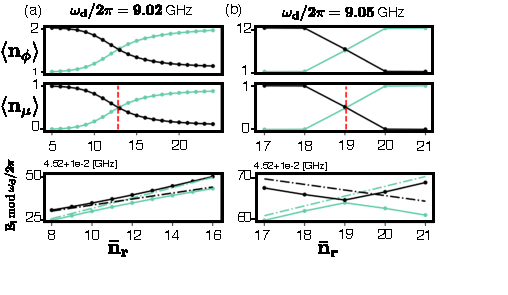
\includegraphics[width=\linewidth]{Figures/Floquet_011.pdf}
    \caption{Examples of p-MIST using transitions \textbf{(a)} $8$ and \textbf{(b)} $9$ from Table~\ref{tab:p-MIST} involving the $\ket{\tilde{1},\tilde{0}}$ state, with maximum overlap to the un-hybridized state $\ket{1}_\phi\otimes\ket{0}_{\mu=2}$. \textbf{Top row:} Qubit mode average occupation $\braket{n_\phi}$. \textbf{Middle row:} Parasitic mode average occupation $\braket{n_\mu}$. \textbf{Bottom row:} Stark-shifted eigen-energies (dashed) from first-order perturbative calculations, and quasi-energies (solid) from Floquet simulations showing avoided crossings. Plots are extracted from numerical data used in Fig.~\ref{fig:Floquet}. The data points are connected by lines for visual aid.}
    \label{fig:011}
\end{figure}
In this section, we estimate the quasienergies and rates of exemplary p-MIST transitions, using the Landau-Zener formalism, respectively. In both the Floquet simulations and Landau-Zener approximations, the spectral gap of an associated transition is a critical figure-of-merit in determining the \singh{adiabatic} energy exchange probability. Figs.~\ref{fig:011}(a,b) respectively show the p-MIST explicit population exchange in transitions $8,9$ from Table~\ref{tab:p-MIST} involving $\ket{\tilde{1},\tilde{0}}$, the state involved in computation as well as readout~\cite{zhang_universal_2021}. The simultaneous exchange of population in the qubit mode $\phi$, shown in the top panels, and the parasitic mode $\mu=2$, shown in the middle panels, confirms that the transitions are indeed p-MIST. 

The bottom panel of Fig.~\ref{fig:011} shows the avoided crossing at the transition point in solid lines. The dashed lines show the eigenenergies calculated in App.~\ref{app:stark-shift} by estimating the Stark shift from the readout drive onto each state. For small drive amplitudes compared to the gaps in the spectrum, the simple estimate of the eigenenergies using perturbation theory as used in App.~\ref{app:stark-shift} is permissible. This is confirmed by the agreement of the dashed and solid lines in the bottom panel of Fig.~\ref{fig:011}(b). For this transition, comparing our second-order Fermi's Golden rule estimate (see App.~\ref{app:Floquet-trans})  to the numerically obtained energy gaps in the quasi-energies (solid lines), we find agreement \singh{within $0.1 \ \mathrm{KHz}$}. The remaining disagreement between the quasi-energies and the estimated eigenenergies suggests that higher-order or non-perturbative corrections become relevant for transitions slower than \singh{$\Delta_{ac}=0.5 \ \mathrm{MHz}$}. Notably, both the transitions shown in Fig.~\ref{fig:011} occur at low average readout photon number of $\bar n_r=11,19$, well within the power typically needed for high signal-to-noise dispersive readout of superconducting qubits~\cite{gusenkova2021quantum}. 

We will now compute the transition probability of the p-MIST effect shown in Fig.~\ref{fig:011}(b). This choice was made based on a larger avoided crossing for (b) $\Delta_{ac}=0.66$ as compared to (a)  $\Delta_{ac}=0.12$.
\begin{figure}[htb]
    \centering
    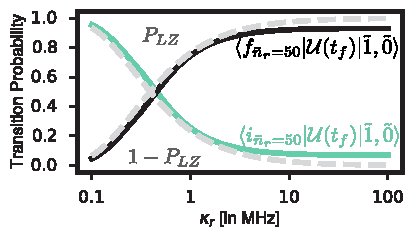
\includegraphics[width=\linewidth]{Figures/LZ.pdf}
    \caption{Adiabatic (green) and diabatic (green) transition probability against the parameter $\kappa_r$ which determines the change in drive strength $\xi_{\mu/\phi}=2g_{\mu/\phi}\sqrt{\bar n_r(t)}$ where $\bar n_r(t)$ follows Eq.~\ref{eq:LZ-n}. Here, $\ket{f_{\bar n_r=50}}$ and $\ket{i_{\bar n_r=50}}$ are the final states in the end of branch analyses for $\ket{\tilde{2},\tilde{1}}$ and $\ket{\tilde{1},\tilde{0}}$, respectively, at $\omega_d=9.05 \ \mathrm{GHz}$. The Landau-Zener probability ($P_{LZ}$) for the avoided crossing in Fig.~\ref{fig:011}(b) is marked in gray.}
    \label{fig:LZ}
\end{figure}
For this analysis, instead of linearly increasing the drive power of a driven fluxonium circuit, we assume a time dependence of the average readout photon number of
\begin{align}
    \bar n_r(t)&:\bar n_r(1-e^{-\kappa_r t/2})^2,\label{eq:LZ-n}
\end{align}
which includes a ring-up time of $1/\kappa$, according to the readout resonator bandwidth~\cite{khezri2023measurement,dumas2024unified,cohen2023reminiscence}. This equation computes the occupation of the readout resonator under a drive with a decay rate of $\kappa_r$. %Note that the time interval $\Delta t$ is computed using $\Delta \bar n_r=1$, thus replicating our previous model used for Floquet simulations with $\bar n_r=50$. 

We first use Hamiltonian dynamics to compute the transition probability as the overlap of the initial state  $\ket{\tilde{1},\tilde{0}}$ evolved under the unitary $U=e^{i\hat H_{s.c.}t}$ with the Floquet branch of the two states $\ket{i}=\ket{\tilde{1},\tilde{0}}$ and $\ket{f}=\ket{\tilde{2},\tilde{1}}$, involved in the transition. The system is evolved for a time $t_f=\frac{10}{\kappa_r}$ such that the readout mode reaches the steady state population. Varying $\kappa_r$ changes the probability of transitions, plotted in Fig.~\ref{fig:LZ}. The overlap with `$i$' represents the probability of an adiabatic transition while the probability of a diabatic transition is given by the curve plotting the overlap against `$f$'. We see that there is a significant probability of an adiabatic transition $\kappa_r\le 1 \ \mathrm{MHz}$, the target readout decay parameter (see Table~\ref{tab:readout_params}). 

We also use the numerically-computed gaps in the quasi-energies at the avoided crossing to evaluate the Landau-Zener (LZ) probabilities $P_{LZ}$, using the method described in Ref.~\cite{ikeda2022floquet} (for details see App.~\ref{app:LZ}). Unlike the case of transmons Ref.~\cite{dumas2024unified} we do not find perfect agreement in these two cases. This indicates that the two-state physics captured by Landau-Zener transitions may not be correct for studying the strengths of most fluxonium transitions. As $\kappa_r\rightarrow \infty$ the states seem to saturate to a superposition of $i-f$ since the green and black curves always sum up to $1$. Note that, similar to the Hamiltonian dynamics the population exchange plots in Fig.~\ref{fig:011}(b) also show that the green and black curves do not saturate to $1,2$ and $0,1$ in the top and bottom panels, respectively.

We have confirmed that an observed p-MIST can have a significant probability during a fluxonium qubit readout. While this effect will directly affect the readout performance for our chosen set of readout parameters, we will now analyze its impact on the qubit coherence.

\subsection{Qubit Dephasing post-Readout} 
Implications of p-MIST can be fatal even \textit{after} the readout pulse is executed, in the context of a larger quantum circuit where the fluxonium mode is used as a qubit. In general, the parasitic modes are long-lived, with internal quality factors of $\sim 10^{4}$~\cite{masluk_microwave_2012, masluk2013reducing}. We have confirmed that dephasing due to the detuned drive and thermal effects is negligible (see App.~\ref{app:dephasing}). However, spurious excited state population of the parasitic mode introduced by p-MIST during readout can induce significant correlated dephasing of the qubit, through the large dispersive interaction $\chi_{\mu \phi}/2\pi \sim 1 \ \mathrm{MHz}$ (see Table~\ref{tab:circuit_params}). If the parasitic mode is excited, the qubit accumulates a phase at a constant rate $\chi_{\mu\phi} \bar n_\mu$, in the absence of any decay i.e. infinite internal quality factor $Q_\mu$. This error can be measured and corrected for, given the knowledge of $\bar n_\mu$. For a finite $Q_\mu$, the parasitic mode decays at a rate $\kappa_\mu=Q_\mu/\omega_\mu$ such that the qubit dephasing is no longer deterministic but a Poissonion process that relies on the random decay of the parasitic mode. Now, we will analyze this effect due to p-MIST-induced excitation in the parasitic modes.


\begin{figure}[htb]
    \centering
    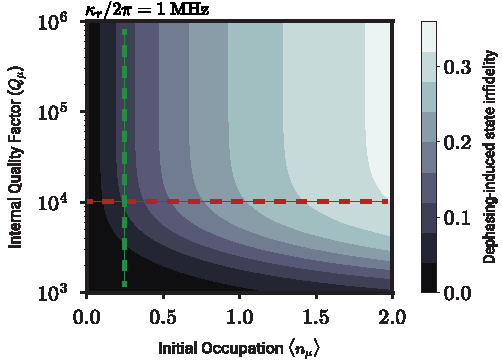
\includegraphics[width=\linewidth]{Figures/dephasing.pdf}
    \caption{Dephasing error probability due to random decay of an excited parasitic mode with occupation $\bar n_\mu$, after p-MIST, for various internal parasitic quality factor $Q_\mu$. The horizontal red line shows the quality factor quoted in~\cite{masluk_microwave_2012}. The green lines show the dephasing error probability for transition $9$ (see Figs.~\ref{fig:011}(b) and~\ref{fig:LZ}) at different average readout photons ($\bar n_r$).}
    \label{fig:dephasing}
\end{figure}

Post the readout pulse in transition $9$ (see Fig.~\ref{fig:011}(b)) for $\kappa_r=1 \ \mathrm{MHz}$, we can reset the fluxonium subspace to, say, the qubit state $\ket{+}=\frac{\ket{0}_\phi+\ket{1}_\phi}{\sqrt{2}}$. The parasitic mode, however, remains excited $\ket{1}_{\mu=2}$ with some probability.
To emulate the effect of this transition, we perform a master equation simulation of a toy model where a disjoint qubit-cavity state $\ket{+,\bar n_\mu}$ is evolved under the Hamiltonian $H=\chi_{\phi\mu} \hat a_\mu^\dagger \hat a_\mu \sigma_z$. During this evolution, the cavity (here, the parasitic mode) suffers dissipation under the decay operator $\sqrt{\kappa_\mu t}\hat a_\mu$. We plot in Fig.~\ref{fig:dephasing} the infidelity of the qubit state with the $\ket{+}$ state, after the parasitic mode reaches a steady state at $T_f=10/\kappa_\mu$, for various $Q_\mu$ and $\bar n_\mu$. Specifically, we find that for an internal quality factor $Q_\mu$ of $10^{4}$ and population of $\braket{n_\mu}=0.5$ in the parasitic mode $\mu=2$ is needed to introduce a dephasing error probability, $\sim 0.2$, which is already past the threshold of surface code decoders~\cite{fowler2012surface}. Given that the population of the parasitic modes is about $\bar n_\mu\sim 0.5$ at a readout power of $\sim 11$ photons, well within the signal to noise ratio~\cite{gusenkova2021quantum}, we expect that qubit coherence can be limited by p-MIST in circuit designs which do not anticipate them.

Thus, we have provided quantitative evidence, with the help of various methods used in these analyses, that p-MIST processes can limit the performance of a fluxonium qubit architecture, without careful consideration of the parasitic modes during circuit design. In the next section, we will analyze the range of various mode frequencies and coupling strengths responsible for these effects.

\section{Effects of Circuit Modifications on p-MIST}\label{sec:expressions}
The p-MIST processes shown in the previous section can be mitigated in various ways, by adjusting the qubit frequency, readout resonator frequency, and parasitic mode frequencies, as well as reducing parasitic mode and qubit coupling strengths. In this section, we explore the impact of each of these components individually. All equations analyzed in this section were derived in Ref.~\cite{viola2015collective} for the circuit in Fig.~\ref{fig:meas_circuit}, and we have extended these results to circuits with different grounding configurations in App.~\ref{app:alt_circuits}.
\subsection{Coupling Strengths} \label{sec:coupling}
The strong coupling between the qubit and the parasitic mode is primarily responsible for p-MIST processes. Here, we show evidence of this, via Floquet simulations where various coupling constants are changed to zero to analyze their significance. Fig.~\ref{fig:coupling-Floquet} compares Floquet plots for the initial state $|\tilde{1}, \tilde{0}\rangle$ under different coupling conditions. Fig.~\ref{fig:coupling-Floquet}(b) shows that $g_{\phi r}$ alone does not cause significant transitions or p-MIST processes without $g_{\phi \mu}$. This is evident from the absence of all parasitic transitions $(8,9)$ and no streak or sharp change in color indicating parasitic mode excitations in the bottom panel. The parasitic mode population in the absence of this coupling is restricted to $\bar n_\mu=10^{-4}$. Turning both parasitic couplings (not shown here) off completely removes any population from the parasitic mode. For full Floquet landscape with quasi-energy see App.~\ref{app:coupling}. Therefore, reducing the coupling strength $g_{\phi \mu}$ is a potential path to mitigating p-MIST processes. 
\begin{figure}[!htb]
    \centering
    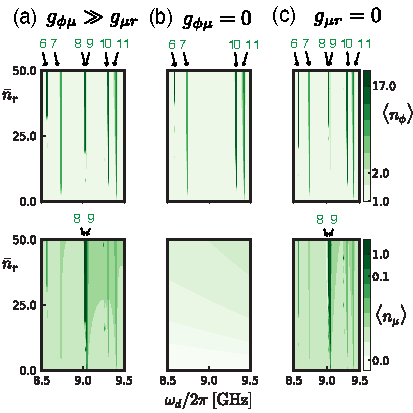
\includegraphics[width=\linewidth]{Figures/Floquet_coupling.pdf}
    \caption{Floquet Simulations for the circuit parameters in Table~\ref{tab:circuit_params} due to the various coupling terms in Eq.~\ref{eq:int_hamiltonian}. The marked transitions show the MIST processes observed in Fig.~\ref{fig:Floquet}. \textbf{(a)} Same as Fig.~\ref{fig:Floquet}(b). \textbf{(b)} Zero parasitic mode coupling to the qubit. \textbf{(c)} Zero parasitic mode coupling to the readout. Same as before the Floquet figures are plotted in log scale for visual aid to the marked transitions.}
    \label{fig:coupling-Floquet}
\end{figure}

Here, we analyze the dependence of these coupling strengths on circuit and readout parameters. As derived in App.~\ref{app:alt_circuits} and given in~\cite{viola2015collective}, the coupling strength $g_{\phi \mu}$ is
\begin{align}
g_{\phi\mu}=\sqrt{\frac{2}{N}} \frac{\tilde{E}^\phi_c\tilde{E}^e_{c,\mu}c_\mu}{E_{g_j}s_\mu^2}     \cdot {N_\phi}_{ZPF} \cdot {N_\mu}_{ZPF}
\end{align}
where $c_\mu=\cos{\frac{\pi\mu}{2(N-1)}}$, $\tilde{E}_c^\phi,\tilde{E}^e_{c,\mu} $ are the qubit and parasitic mode charging energies, respectively, and $N_{\phi/\mu,ZPF}$ are the zero-point fluctuation values for the qubit and parasitic modes. Expressions for $\tilde{E}^e_{c,\mu}$ can be found in Eq.~\ref{eq:parasitic}, $\tilde{E}_c^\phi,N_{\phi/\mu,ZPF}$ can be found in App.~\ref{app:Hamiltonian} while all the other parameters are given in Table~\ref{tab:circuit_params}. 

By observation, suppressing the parasitic capacitance to ground near the junction array suppresses the qubit-parasitic coupling $g_{\phi\mu}$. However, this is constrained by practical limits of around $0.1$ fF per junction due to the gap to the ground plane. For the parasitic modes with the strongest coupling to the qubit $\mu\ll N$. The large $N$ limit with $c_\mu\approx 1$ yields
\begin{align}
    \tilde{E}^e_{c,\mu}\approx E_{g_j}s_\mu^2, \quad \tilde{E}^\phi_c\propto \frac{1}{N^2}\implies g_{\phi\mu}\propto \frac{1}{N^{5/2}}.
\end{align}
 These dependencies are plotted in Fig.~\ref{fig:circuit_comp} of App.~\ref{app:Hamiltonian}. The trend concerning $N$ is not so straightforward.  Note that changing $N$ changes the target inductance of the qubit. Keeping the same inductance as $N$ changes requires one to increase $E_{J_j}$ by the same factor as $N$. To keep the $E_{J_j}/E_{C_j}$ ratio the same this leads to an increase in $E_{C_j}$, thus extending our argument for large $N$ even further. Thus, both these tasks (increasing $N$, decreasing $C_{g,j}$) are hard at hand.  

\subsection{Mode Frequencies}\label{mode-frequencies}
 We can estimate the resonance conditions for a p-MIST effect by identifying  energy-conserving processes, where $x$ photons are converted into a transition $\tilde{\Delta}_{if,y}$ in the hybridized eigenspace of the fluxonium and parasitic mode $\mu=2$. Here, $\tilde{\Delta}_{if,p}$ is the transition energy between levels $\ket{\tilde{i},\tilde{m}}$ and $\ket{\tilde{f},\tilde{n}}$ such that $|m-n|=y$. In the disjoint Hilbert space, this equation can also be interpreted as a process where $x$ readout photons convert into $y$ parasitic mode photons and a fluxonium excitation $\ket{i}_\phi \leftrightarrow \ket{f}_\phi$ where $\Delta_{if}=|E_f-E_i|$. To guide intuition for understanding the spectrum of resonance conditions, we plot such energy-conserving processes in Fig.~\ref{fig:trans_prof}, for the lowest-order case of $\mu=2$, that satisfies $|x\omega_r-\tilde{\Delta}_{if,y}|\le 25 \textrm{ MHz}$ which, in the disjoint Hilbert space approximates to,
\begin{align}
|x\omega_r-(y\omega_\mu+\Delta_{if})|\le 25 \textrm{ MHz}.
\label{eq:En_cons}
\end{align}
Here, a buffer of $25 \ \mathrm{MHz}$ is allowed to accommodate for Stark shift (see App.~\ref{app:stark-shift}).
\begin{figure}[!htb]
    \centering
    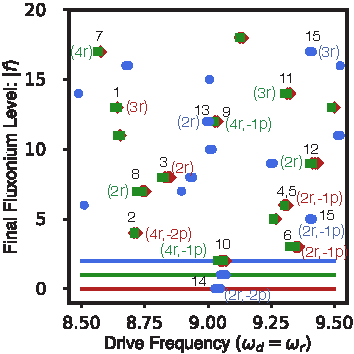
\includegraphics[width=\linewidth]{Figures/Trans_.pdf}
    \caption{Energy conserving processes $\ket{\tilde{i},\tilde{0}}\leftrightarrow\ket{\tilde{f},\tilde{y}}$ for Eq.~\ref{eq:En_cons} for $x\le 4, y\le 2, j\le 20$ and $i=0$ (red diamonds), $i=1$ (green squares), $i=2$ (blue circles). The horizontal lines indicate the initial state for each color for visual aid. Labels in black correspond to transition $\#$ listed in Table~\ref{tab:p-MIST}. Colored labels ($x \mathrm{r},-y \mathrm{p}$) show the number of readout photons absorbed ($x$) and the number of parasitic mode ($\mu=2$) photons emitted ($y$) in the transition. The faded points are processes not captured in the Floquet simulations.}
    \label{fig:trans_prof}
\end{figure}

The energy profile in Fig.~\ref{fig:trans_prof} shows us the regions where up to four-readout-photon processes will be prominent when starting in one of the four lowest fluxonium levels involved in the readout. Note that there are downward transitions from $\ket{2}_\phi$ to $\ket{1}_\phi,\ket{0}_\phi$ in the fluxonium subspace, in the presence of parasitic modes, one of which was captured in transition $15$ of Table~\ref{tab:circuit_params}. To emphasize the correctness of these predictions we label in black all the transitions captured in the Floquet simulations (see Sec.~\ref{sec:MIST}) in Fig.~\ref{fig:trans_prof}) while the processes not captured here are faded. The parenthesized labels on color denote the number of readout photons ($x \mathrm{r}$) and parasitic mode photons ($y\mathrm{p}$) required for the transition in the fluxonium subspace, where a positive index denotes absorption while a negative index denotes emission. These labels correspond to the disjoint subspaces for simplified representation but the energy conservation uses the eigen-energies of the hybridized eigenstates of $H_{0}$ (see Eq.~\ref{eq:bare_ham}). For example, transition $2$ emits $4$ readout photons which are converted into $2$ parasitic mode photons, absorbed by the mode $\mu=2$, and the transition $\ket{0}_\phi\leftrightarrow \ket{4}_\phi$ in the fluxonium subspace. The equation indicates that a large gap between $\omega_d$ and $\omega_\mu$ would require a large $m$ to trigger a p-MIST effect. We verify this intuition for different ranges of the various mode frequencies. 

\paragraph{Drive Frequency ($\omega_d$):} If $\omega_d\gg \omega_{\mu=N-1}$, the most fatal case would be excitation of a strongly coupled low-frequency parasitic mode to large $n$ leaving just enough energy to produce excitation $f$ in the Fluxonium subspace of significant charge matrix elements (see Fig.~\ref{charge-matrix}). However such large excitations in the parasitic modes would be less probabilistic. A proper investigation of this case requires a large Hilbert space and is beyond the scope of this work. A low frequency readout, on the other hand, would incur a large $m$ and can have similar impact. We give the Floquet figure corresponding to a low frequency readout in Fig.~\ref{fig:Flo_low} which looks severely more populated compared to Fig.~\ref{fig:Floquet}. It is important to compare the rates of such transitions, however, the increase can be explained around $6 \ \mathrm{GHz}$. The rear end of this frequency range is the same as the plasmon energy and half the parasitic mode $\mu=2$ frequency. This logic already indicates that $5.5-6 \ \mathrm{GHz}$ would be a bad range of frequencies for the current choice of parameters. However, for the purpose of readout, a lower $\omega_d$ is not favorable due to thermal effects, and hence not analyzed further in this work.  

\begin{figure}[htb]
    \centering
    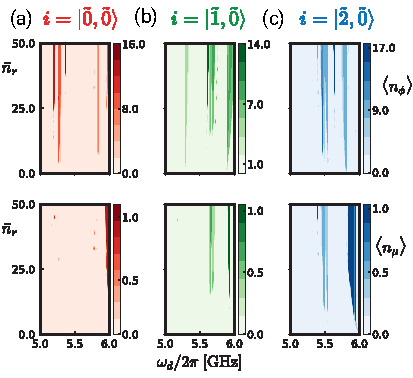
\includegraphics[width=\linewidth]{Figures/Floquet_low.pdf}
    \caption{Floquet simulations at lower readout frequencies using circuit parameters quoted in Tables~\ref{tab:circuit_params} and~\ref{tab:readout_params} for branch analysis starting in the dressed hybridized eigenstate $i=\ket{\tilde{k},\tilde{0}}$, with maximum overlap to the un-hybridized states $\ket{k}_\phi\otimes\ket{0}_{\mu=2}$. The figures are plotted in linear scale, unlike Fig.~\ref{fig:Floquet}, making any streak due to significantly weaker transitions \singh{($\Delta_{ac}<1 \ \mathrm{KHz}$)} unnoticeable.}
    \label{fig:Flo_low}
\end{figure}

\paragraph{Parasitic Mode Frequency:}
Another approach towards mitigating p-MIST processes is to adjust $\omega_\mu$ so that $\omega_\mu \gg\omega_r$ for $\mu=2$, potentially improving the circuit. This is feasible with granular-aluminum (GrAl) inductive shunts, though they are lossy~\cite{gusenkova2021quantum}. Recent efforts are being applied towards improving GrAl shunts. 

For the JJA parameters, to provide some quantitative arguments in this direction we discuss the dependency of $\omega_\mu$ for even parasitic modes ($e$) on various circuit variables. 
\begin{align}
    \frac{\omega_\mu^e}{2\pi}&=\sqrt{8E_{c,\mu}^e E_{J_j}},\quad\text{where}\\
    E_{c,\mu}^e&=\Big[\frac{1}{E_{C_j}}+\frac{1}{4E_{g_j}s_\mu^2}\Big]^{-1}.\label{eq:parasitic}
\end{align}
Here, $s_\mu = \sin (\frac{\pi \mu}{2(N-1)})$. Here, $E_{c,\mu}^e$ is the charging energy of an even parasitic mode. All other variables used are defined in Table~\ref{tab:circuit_params}. For parasitic modes with strong coupling, $\mu\ll N$, for large $N$, the charging energy is $\tilde{E}^e_{c,\mu} \approx 4E_{g,j} s_\mu^2$, which is inversely proportional to $N^2$ and directly proportional to $E_{g_j}$. Again, a smaller parasitic ground capacitance $C_{g_j}$ increases the parasitic mode charging energy, and thus desirably increasing its frequency. However, in contrast with the case of coupling strength $g_{\phi\mu}$, a larger $N$ leads to lower frequencies for these modes, which is unfavorable. Fig.~\ref{fig:circuit_comp} in App.~\ref{app:Hamiltonian} shows the dependence of charging energy of parasitic modes as well as qubit modes with respect to parasitic ground capacitance. 
As stated before in Sec.~\ref{sec:coupling}, the ground capacitance $C_{g,j}$ is fixed while the impact of decreasing $N$ would require consideration of nonlinear corrections as well as fixed inductance, thus, again making these changes difficult. 


In the previous sections we focused on $\sim 30 \ \mathrm{MHz}$ fluxonium frequency. To extend our results to other experiments, we consider another circuit inspired by parameters in~\cite{ding_high-fidelity_2023} and show p-MIST processes in a $236 \ \mathrm{MHz}$ fluxonium. The parasitic mode frequency of the $\mu=2$ mode is $\omega_{\mu=2}=15.51 \ \mathrm{GHz}$. The coupling strengths are as follows, $g_{\phi r}=37 \ \mathrm{MHz}$, $g_{\phi\mu}=216 \ \mathrm{MHz}$, $g_{\mu r}=6 \ \mathrm{MHz}$. The plasmon frequency is $\omega_{12}=5.40 \ \mathrm{GHz}$. Importantly, here we only plot results for $\ket{\tilde{0},\tilde{0}}$ and $\ket{\tilde{1},\tilde{0}}$ because given Ref.~\cite{ding_high-fidelity_2023} uses only the first two levels for readout as well as computation. The detailed circuit parameters are given in App.~\ref{app:alt_circuit1}. The truncation for the simulation of this alternate circuit is discussed is shown in App.~\ref{app:alt_circuit1}. Even though the coupling strengths for these circuit parameters are on par with Table~\ref{tab:circuit_params}, since the parasitic mode frequency of the even mode $\mu=2$ is larger by $\sim 4 \ \mathrm{GHz}$, we expect fewer p-MIST processes in the drive frequency range analyzed in Fig.~\ref{fig:Floquet}. 

\begin{figure}[htb]
    \centering
    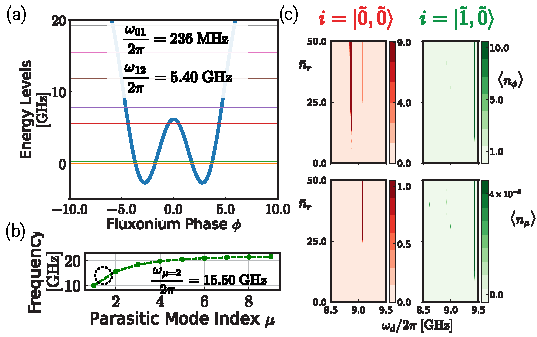
\includegraphics[width=\linewidth]{Figures/Floquet_Will.pdf}
    \caption{Floquet analysis with alternate JJA fluxonium parameters. \textbf{(a)} Fluxonium energy spectrum. \textbf{(b)} Parasitic mode frequencies. \textbf{(c)} Floquet simulations for the branch analysis of the computational states~\cite{ding2023high}. Circuit parameters for this circuit are discussed in Sec.~\ref{mode-frequencies} and App.~\ref{app:alt_circuit1}. The Floquet figures are plotted in linear scale unlike Fig.~\ref{fig:Floquet}, making any streak due to significantly weaker transitions \singh{($\Delta_{ac}<1 \ \mathrm{KHz}$)} unnoticeable.}
    \label{fig:Floquet1}
\end{figure}

Fig.~\ref{fig:Floquet1} shows that the ratio of observed MIST ($3$) and p-MIST ($1$) effects is indeed lower for this alternate circuit. In fact, the one p-MIST observed in the Floquet profile $\ket{\tilde{0},\tilde{0}}\leftrightarrow\ket{\tilde{4},\tilde{1}}$ occurs at $\bar n_r=25$ and has the quasi-energy gap of $\Delta_{ac}=0.13 \ \mathrm{MHz}$ at the avoided crossing. This transition, thus, seems comparable rate to transition $8$ (see Fig.~\ref{fig:011}(a)) which is much weaker compared to transition $9$ (see Fig.~\ref{fig:011}(a)), as observed in Sec.~\ref{sec:LZ}. The corresponding Landau-Zener probabilities and explicit transitions with quasienergies for the Floquet profile in Fig.~\ref{fig:Floquet1} can be found in App.~\ref{app:alt_circuit1}. However, a detailed understanding of this Floquet profile, including rate calculations, is necessary to make proper claims in relation to severely reduced MIST processes, and is left as future direction.

\section{Conclusion and Further Work}\label{sec:conclusion}
%%%%Summary/inferences&&&&&&
In this work, we have analyzed the impact of parasitic modes on driven JJA fluxonium qubit. This work shows that transitions in a fluxonium circuit triggered by a parasitic mode of the JJA can occur with considerable rates from coupling of the parasitic modes with the qubit mode. Our results, while simulated for a driven fluxonium circuit can give intuition related to MIST processes during a readout pulse. We show this simplification from the readout circuit Hamiltonian and justify that our claims hold for readout induced state transitions. The parallel circuit considered in this work utilizes a specific symmetry which removes the coupling between the lowest frequency mode and the qubit. We show that this symmetry is preserved even if the readout resonator is coupled to a floating or grounded fluxonium at a single point. Our analysis considers fluxonium at the sweet spot which introduces additional symmetries forbidding transitions between parity-conserving states via first-order transitions. Despite these various symmetries and our modest assumption of no self-nonlinearity in the JJA or the readout, our results show that a strong coupling of parasitic modes to the qubit mode still triggers parasitic transitions at low average readout photons. We call these transitions parasitic-MIST or p-MIST, inspired by the term MIST for measurement-induced-state-transitions. Not only does p-MIST lower the onset of MIST processes to $\sim 10$ readout photons but it also significantly dephases the qubit, both of which directly limit the readout fidelity~\cite{hazra2024benchmarking}. 


%%%%Extension of our assumptions%%%%
We analyze the trend in p-MIST for various drive frequencies, parasitic mode frequencies, coupling constants, and circuits with two different qubit frequencies equal to $\sim 30$ and $\sim 300 \ \mathrm{MHz}$. The assumptions we make are crucial to our MIST analysis. Increasing $N$ can reduce the nonlinearity of the parasitic modes, with insights provided in Sec.~\ref{sec:expressions}. We also neglect the self-nonlinearity of the readout mode which has been a common practice in recent MIST-related analysis~\cite{shillito2022dynamics,dumas2024unified,cohen2023reminiscence}. While the effects of nonlinearity in parasitic and readout modes can have significant impact on the readout fidelity, Floquet simulations including self-nonlinearity of these modes is beyond the scope of our work. Analysis of a disordered array could also be an interesting extension of our work as it may lead to lower coupling between the qubit and the parasitic modes. 

%Our work reveals that collective modes in a Josephson junction array can limit fluxonium qubit readout. Specifically, the simultaneous coupling of the second-order parasitic mode with the qubit and the readout modes allows two-photon absorption to alter both the fluxonium and parasitic modes. This effect is demonstrated using standard circuit parameters, following typical parameter values for long lifetimes of the fluxonium qubit, qubit frequencies of $\sim 100 \ \mathrm{MHz}$ for facilitating microwave driving, and practical considerations for stray capacitive couplings to ground near the junction array. For example, with our specific choice of circuit parameters, we find that the onset of excitations of the parasitic mode and fluxonium qubit effectively limits the readout power to about $\sim 10$ photons, well within the desired power for high signal-to-noise ratios \cite{gusenkova2021quantum}.\sh{Emma, is this citation correct?} We achieve this result through a detailed analysis of the circuit Lagrangian, covering the internal modes of junction array, the readout resonator, and the fluxonium qubit. %Our Floquet simulations, supported by a perturbative Hamiltonian analysis, are modified from~\cite{dumas2024unified} to avoid supercomputing needs. We confirm that our results hold for both parallel circuits as well as single-point connections with floating and grounded fluxonium circuits. Finally, we explore how variations in junction count and ground capacitances can affect the readout fidelity.

To advance practical implementation and reduce fluxonium MIST in the dispersive readout, we suggest adding noise to the Floquet framework~\cite{huang_engineering_2021} and linking our results to readout fidelity values using input-output theory. Future work should also incorporate the intrinsic nonlinearity of both the junction array modes and the readout mode. Mitigating parasitic mode excitations could involve varying junction energies along the array to localize collective modes, thereby altering the parasitic mode spectrum and reducing excitation probability. Alternative readout schemes like longitudinal readout or cloaking could also be explored~\cite{reed_high-fidelity_2010, munoz-arias_qubit_2023, didier_fast_2015}. Given the strong coupling between parasitic modes and fluxonium, these modes could potentially enhance fluxonium qubit readout. We propose using a feedline with a Purcell filter to tailor the spectrum and protect the qubit, reducing capacitive loading constraints.


Our results present a first analysis toward understanding the role of parasitic modes in the readout dynamics of a fluxonium circuit. Although the circuit parameters used in this work are closest to a fluxonium circuit, these results can be generalized to other high-anharmonic superconducting circuits with similar mode frequencies.

\section{Acknowledgments}
 We thank Akshay Koottandavida, Daniel K Weiss, Connor Hann, Kyungjoo Noh, and Simon Leiu for fruitful discussions. We are grateful to Simone Severini, Bill Vass, Oskar Painter, Fernando Brand\~ao, Eric Chisholm, and AWS for supporting the quantum computing program. %SS acknowledges support from the Army Research Office (ARO) under Grant Number W911NF-23-1-0051 for the time she spent on this project at Yale. SS is grateful to Connor Hann for inviting her to pursue an internship program at AWS where this project started.
\appendix
\section{Single-Point Connections}\label{app:alt_circuits}
%Appendices for Sec 4
\begin{figure*}[htb]
    \centering
    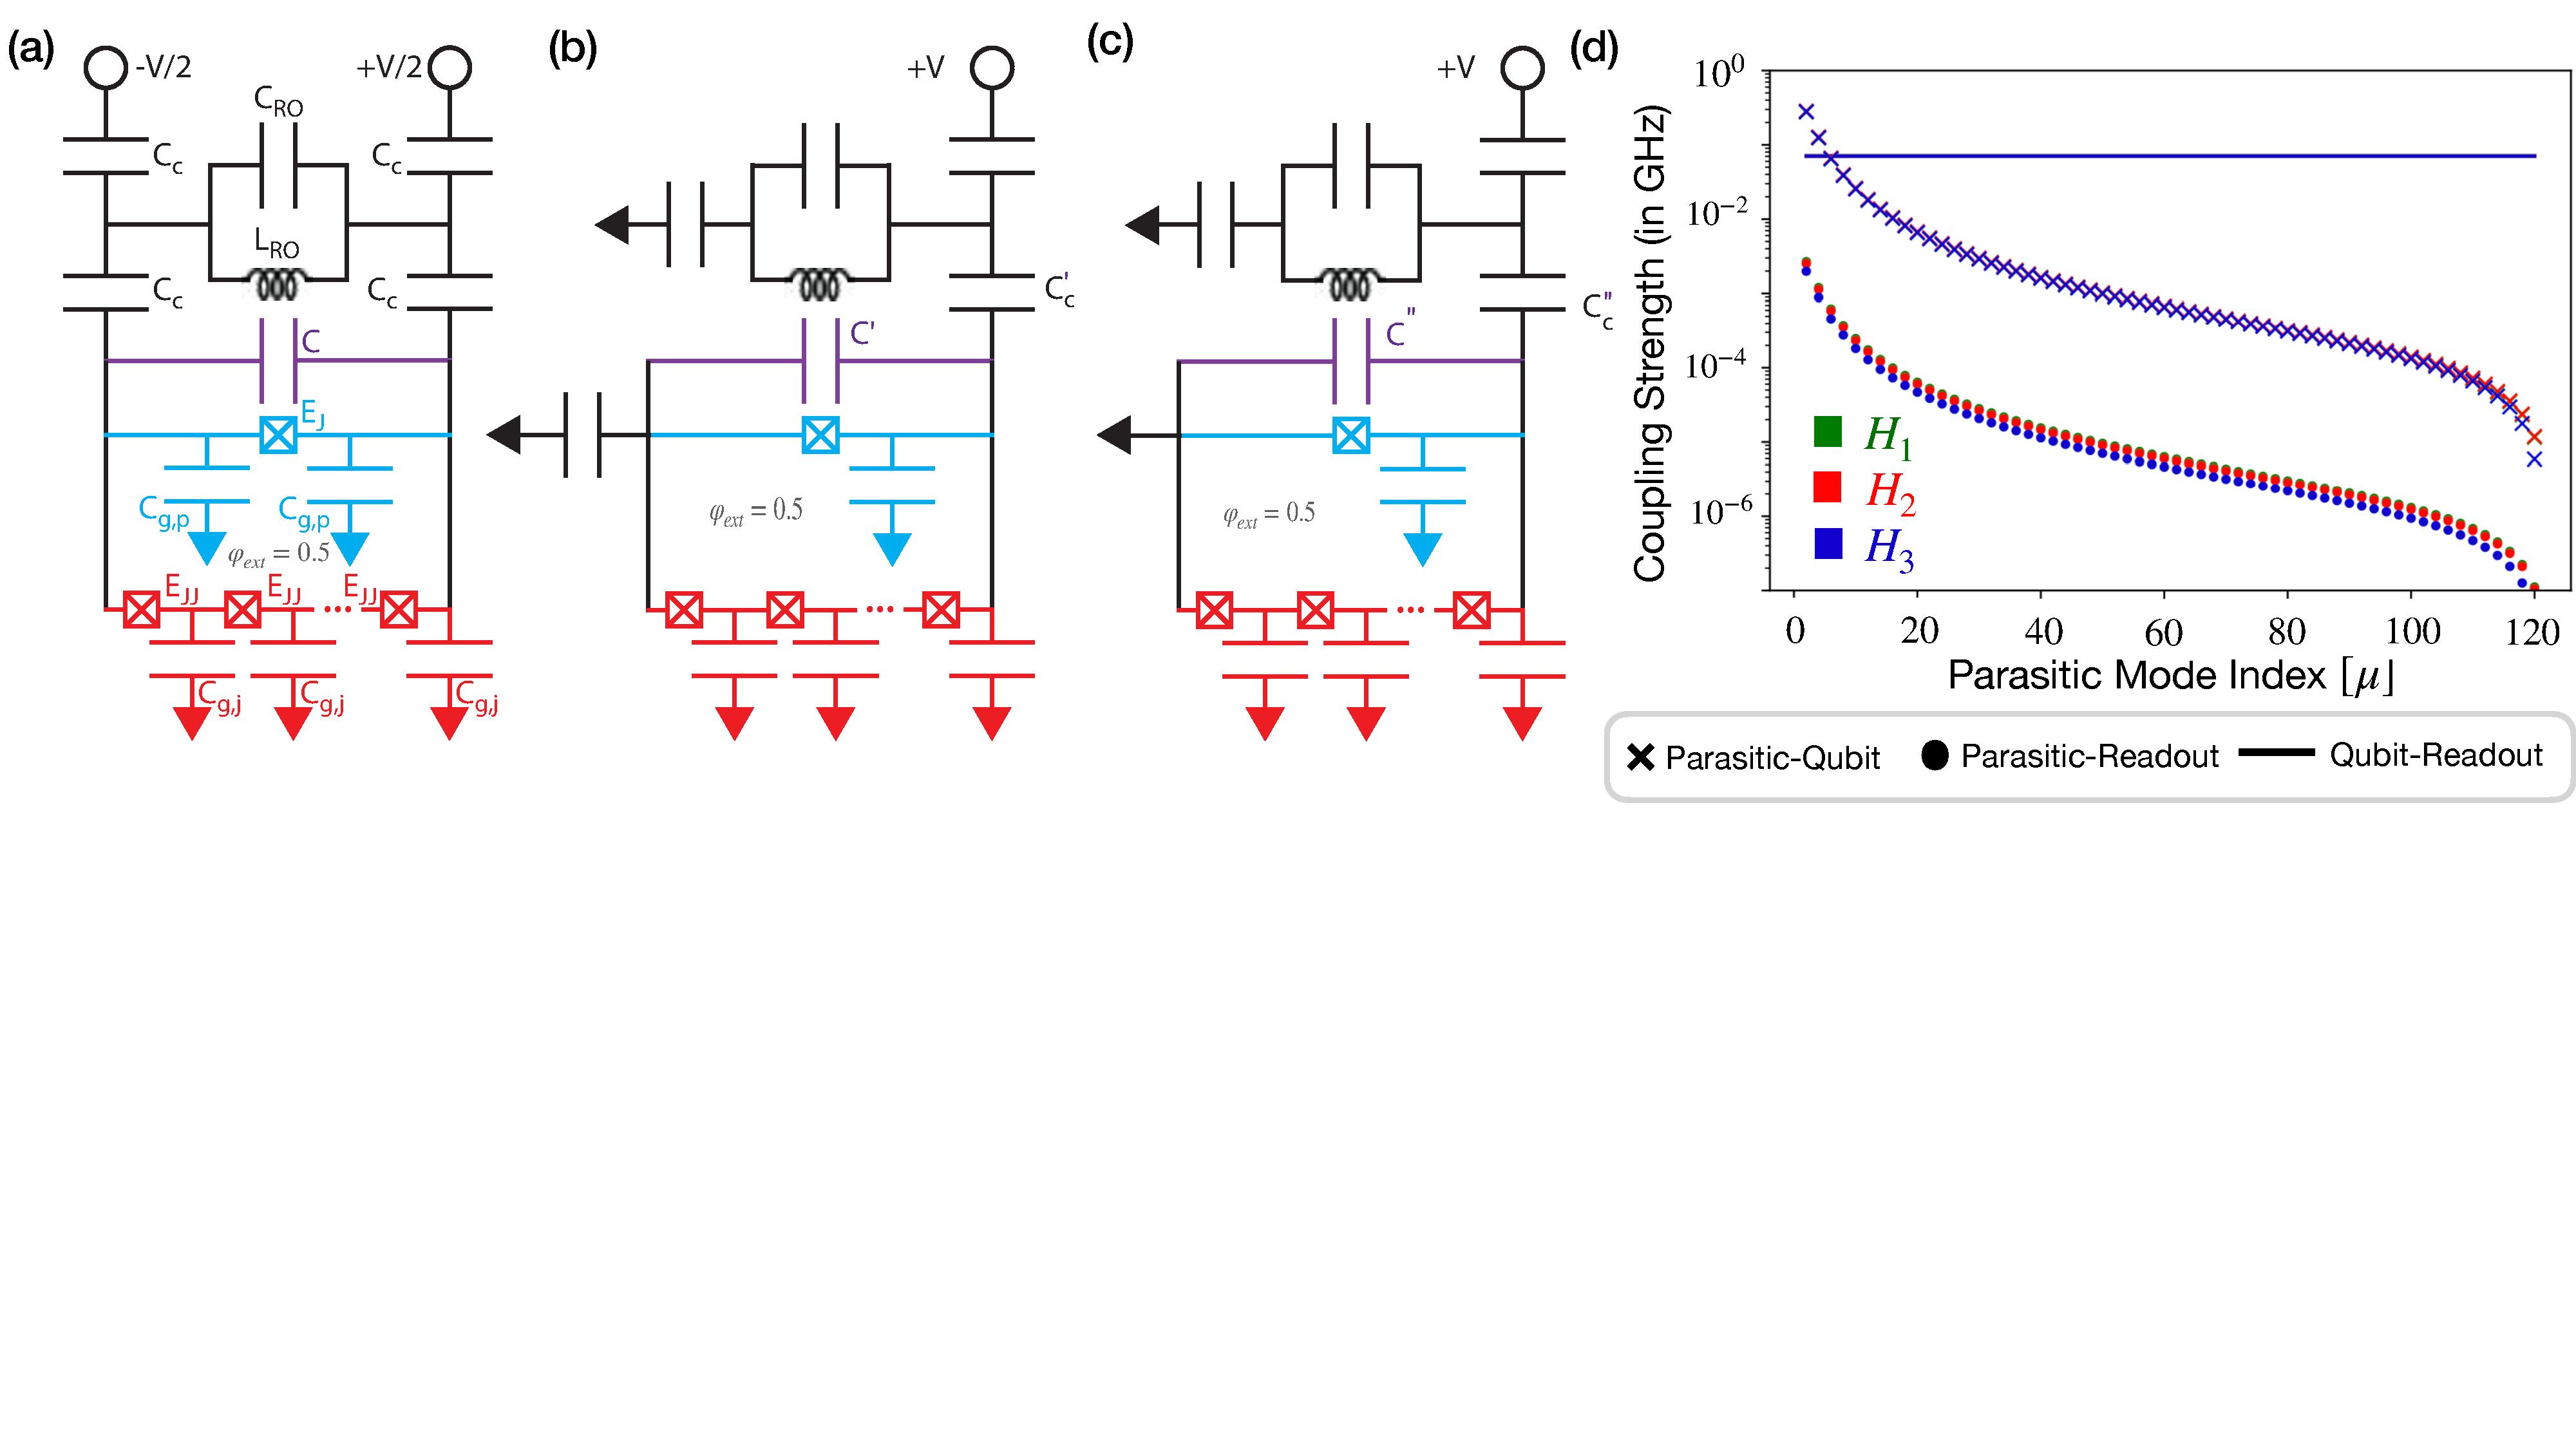
\includegraphics[width=\linewidth]{Figures/Circuit_choice.pdf}
    \caption{(a-c) Alternative readout circuits. (a) Parallel circuit, (b) Floating fluxonium, (c) Grounded fluxonium. Alternatives (b) and (c) require a single-point connection to the readout line $V$, unlike the parallel circuit in (a). We maintain the values for all circuit variables the same as used for the case of the parallel circuit in Fig.~\ref{fig:meas_circuit}. (d) Absolute values of the coefficients of coupling terms in the Hamiltonian (in GHz). We can see that the parasitic modes couple to the qubit stronger than the qubit couples to the readout. The parasitic mode coupling to the readout is very slightly weaker in $H_3$ compared to $H_1$, $H_2$.}
    \label{fig:circuit_choice}
\end{figure*}

\begin{table}[!htb]
    \centering
    \begin{tabular}{|c|c|c|c|}
    \hline
     \shortstack{\\\textbf{Fluxonium}\\ \textbf{Parameters}\\$(\mu=2)$} & \shortstack{$H_1$\\\textbf{Parallel}\\\textbf{Circuit}} & \shortstack{$H_2$\\\textbf{Floating}\\\textbf{Fluxonium}}& \shortstack{$H_3$\\\textbf{Grounded}\\\textbf{Fluxonium}}\\
\hline
         $g_{\phi \mu}$&$157 \ \mathrm{GHz}$&$161 \ \mathrm{GHz}$& $158 \ \mathrm{GHz}$\\
\hline
         $g_{\mu r}$&$4.223 \ \mathrm{MHz}$&$3.971 \ \mathrm{MHz}$& $3.128 \ \mathrm{MHz}$\\
    \hline
$\chi_{\phi,\mu}$&-$1.1 \ \mathrm{MHz}$ & -$1.3 \ \mathrm{MHz}$&-$1.1 \ \mathrm{MHz}$ \\\hline
         $\delta\omega_{01,\mu}$&$0.4 \ \mathrm{MHz}$ & $0.45 \ \mathrm{MHz}$& $0.41 \ \mathrm{MHz}$ \\\hline
    \end{tabular}
    \caption{Fluxonium parameters with the lowest frequency parasitic mode with non-zero coupling to the qubit and readout $\mu=2$. Here we quote the frequency of the fluxon transition between the lowest two levels ($\omega_{01}$) and the plasmon transition between the first and second levels ($\omega_{12}$). For the dispersive Hamiltonian obtained for each circuit in Fig.~\ref{fig:circuit_choice}(a-c), we quote the dispersive shift due to readout as $\chi_r$. The values in this table have been experimentally verified for $H_1$. The frequency of this mode is $f_\mu=12.063 \ \mathrm{GHz}$. We give the coupling strengths between the qubit-readout $g_{\phi\mu}$, readout-parasitic $g_{\phi r}$, parasitic-qubit  $g_{\mu r}$ modes. We also give the stark shift $\chi_{\phi\mu}$ and frequency correction $\delta\omega_{01,\mu}$ on the two-level system realized by this fluxonium circuit in the dispersive regime. Here the values of $g_{\phi r}, \chi_{\phi r}, \omega_{\mu=2}$ have been verified experimentally for $H_1$.}
    \label{tab:parasitic_params}
\end{table}

The fluxonium readout circuit shown can have several modifications and each can affect various parameters associated with the efficiency of a fluxonium readout circuit as we proceed to show in this work. Here, in Fig.~\ref{fig:circuit_comp} we present two modifications to the parallel circuit shown in Fig.~\ref{fig:meas_circuit} with different grounding options for the fluxonium circuit. We will refer to these three circuit choices as $H_1:$ (Parallel circuit, see circuit in Fig.~\ref{fig:meas_circuit}), $H_2:$ (Floating fluxonium, see left circuit in Fig.~\ref{fig:circuit_comp}), $H_3:$ (Grounded fluxonium, see right circuit in Fig.~\ref{fig:circuit_comp}). Note that each parameter in Table.~\ref{tab:parasitic_params} is significantly different for the three circuits. We adjust the coupling capacitance $C_c$ and the total capacitance of the phase slip junction $E_{C_p}$ (by modifying $C'$) to achieve the same qubit frequency $\omega_{01}$, plasmon frequency $\omega_{23}$, qubit-readout coupling constant $g_{\phi \mu}$ and qubit-readout dispersive shift $\chi_{\phi r}$ for the three circuits as given in Table~\ref{tab:circuit_params}. These modifications yield for circuit (b)$E_{C_p}=0.83  \textrm{ GHz},E_{C_c}=3.82\textrm{ GHz}$ (c) $E_{C_p}=0.80\textrm{ GHz},E_{C_c}=4.70\textrm{ GHz}$. Table.~\ref{tab:parasitic_params} gives values of the various circuit parameters across the three circuits computed analytically using the expressions given in App.~\ref{app:Hamiltonian}. We note that upon adjusting the qubit parameters, all circuit parameters are similar in the three circuits. We find that, if the differential capacitance $C$ and coupling capacitance $C_c$ are altered such that qubit frequency and qubit-readout coupling are same across all three circuits, the parasitic mode effects are bound to have the same effect given our assumptions of ordered array and no self-nonlinearity in parasitic modes. Hence, we do not expect any change in the MIST/p-MIST processes for single-point connected circuits in the hangar geometry in comparison to what has already been shown in this work.
To emphasize this, we plot the three types of coupling strengths across all circuits in Fig.~\ref{fig:circuit_choice}(d) while other parasitic parameters are given in Table.~\ref{tab:parasitic_params}. Note that, this symmetry prevents any coupling with the lowest-frequency parasitic mode ($\mu=1$) in all three circuits, presence of which would have been potentially detrimental. 

Here we will follow the recipe of Ref.~\cite{viola2015collective} to derive Hamiltonians for circuits shown in Figs.~\ref{fig:circuit_comp}(b,c). We will use the following notations defined in Table~\ref{tab:params}. The Lagrangian corresponding to these circuits is a combination of the Lagrangians, $\mathcal{L}_g$ from the phase-slip junction (comprising of the junction with $E_J/E_C\sim 5-8$ and the capacitor $C$), $\mathcal{L}_{g}$ from the ground capacitances, $\mathcal{L}_{R}$ from the readout resonator and $\mathcal{L}_c$ due to the coupling capacitances $C_c$ and the external voltage $V$. We mark the flux points across JJA using $\varphi_0$ and $\varphi_{N}$. We write the capacitive energy terms using $E_x=\frac{e^2}{2C_x}$ and the voltages of each island $\dot{\varphi}/2e$, such that, $\frac{1}{2}C\frac{\dot{\varphi}^2}{4e^2}=\frac{\dot{\varphi}^2}{16E_C}$. For simplicity, we have $C_{g,i}=C_g\quad\forall i$. The flux variables and voltage variables in the circuit are denoted by $\varphi_n=2\pi\Phi_n/\Phi_0$ and $\dot{\varphi}_n=2\pi V_n/\Phi_0$, respectively, where $\Phi_0=h/2e$ is the superconducting flux quantum. We will use subscripts $j, p$ for JJA and the phase-slip junction coordinates, respectively. The capacitance associated with the phase-slip junction is given by $\frac{1}{E_{C'}}=\frac{1}{E_C}+\frac{1}{E^{j}_{C}}$.

\subsection{Floating Fluxonium Circuit}
For $H_2$, Transforming the Lagrangian in Ref.~\cite{viola2015collective}, the following terms will remain the same in the case of floating fluxonium circuit, given the diagrams in the following sections.
\begin{align}
    \mathcal{L}&=\mathcal{L}_{phase-slip}+\mathcal{L}_{JJA}+\mathcal{L}_{g}+\mathcal{L}_{R}+\mathcal{L}_{C}\\
    \mathcal{L}_{phase-slip}&=\frac{(\dot{\varphi}_N-\dot{\varphi}_0)^2}{16E_{C'}}-E_{J_p}\cos(\varphi_0-\varphi_{N}+\varphi_\mathrm{ext})\\
    \mathcal{L}_{JJA}&=\sum_{n=1}^N\frac{(\dot{\varphi}_n-\dot{\varphi}_{n-1})^2}{16E^{n}_{C_j}}-E^{n}_{J_j}\cos(\varphi_n-\varphi_{n-1})\\
    \mathcal{L}_{R}&=\frac{\dot{\varphi}_{-}^2}{16E_{{R}}}-\frac{\varphi_{-}^2}{16E_{R}}\\
    \mathcal{L}_{g}&=\sum_{n=0}^N \frac{\dot{\varphi_n}^2}{16E^n_{g}}\label{eq:float-float}
  \end{align}
  Here, we will not assume that the capacitances to transmission line are infinite or that ground capacitance for the phase-slip junction and JJA. We will leave the value of $\varphi_{\pm}$ a variable in this case unlike the parallel circuit study we performed above.


\begin{align}
\mathcal{L}_{c}&=\frac{(\dot{\varphi}_{-1}-\dot{\varphi_0})^2}{16E^1_{c}}+\frac{(\dot{\varphi}_{-1}-eV)^2}{16E^3_{c}}+\frac{(\dot{\varphi}_{-2})^2}{16E^4_{c}},\\ &=\frac{\dot{\varphi}^2_0}{16E^1_c}+\frac{\dot{\varphi}^2_{-1}}{16}\Big(\frac{1}{E^1_c}+\frac{1}{E^3_c}\Big)+\frac{\dot{\varphi}^2_{-2}}{16E^4_c}\nonumber\\&\quad-\frac{\dot{\varphi}_0\dot{\varphi}_{-1}}{8E^1_c}-\frac{\dot{\varphi}_{-1}eV}{8E^3_c}+\mathcal{O}(V^2)
\end{align}
Here, $E_c^4$ is the capacitance via which the readout resonator is grounded. Using the basis of (guage-invariant) phase difference, 
\begin{align}
\varphi_m-\varphi_0&=\sum_{l=1}^m\theta_l\\ \sum_{m=0}^N \theta_m+\varphi_\mathrm{ext}&=2\pi z, \quad z\in\mathbb{Z}\quad\text{``fluxoid quantization"}\\
\varphi_\mathrm{ext}&=\pi,    
\end{align}
\paragraph{Lagrangian} 
From using Eq.~\ref{eq:float-float}, we find that, 
\begin{align}
    \dot{\varphi}_0&=E_t\Big(\frac{\dot{\varphi}_{-1}}{E_c^1}-\sum_{n=1}^N\sum_{m=n}^N\frac{\dot{\theta}_n}{E^m_g}\Big)\\&\quad\text{where}\quad E_t=\Big(\frac{1}{E_c^1}+\sum_{n=0}^N\frac{1}{E^n_g}\Big)^{-1}\nonumber\\
\therefore     \mathcal{L}_g+\mathcal{L}_c&=\frac{\dot{\varphi}_{-1}eV}{8E^3_c}+\frac{\dot{\varphi}^2_{-1}}{16}\Big(\frac{1}{E^1_c}\Big(1-\frac{E_t}{E_c^1}\Big)+\frac{1}{E^3_c}\Big)\nonumber\\&\quad+\sum_{n=1}^N\frac{\dot{\varphi}_{-1}\dot{\theta}_n}{E_c^1}\Big(\sum_{i=n}^N\frac{E_t}{8E^i_g}\Big)\nonumber\\&\quad+\sum_{m=1}^N\sum_{n=1}^N\dot{\theta}_m\dot{\theta}_{n}\Big( \sum_{j=\text{max}\{m,n\}}^N\frac{1}{16E_g^j}\Big)\nonumber\\&\quad\quad\Big(1-\sum_{i=\text{min}\{m,n\}}^N\frac{E_t}{E_g^i}\Big)
\end{align}
We simplify the Lagrangian $\mathcal{L}_g+\mathcal{L}_c$ as
\begin{align}
    &=\frac{\dot{\varphi}_{-1}eV}{8E_c}+\frac{\dot{\varphi}^2_{-1}}{16}\Big(\frac{1}{E_c}\Big(1-\frac{E_t}{E_c}\Big)+\frac{1}{E_c}\Big)\nonumber\\&+\sum_{n=1}^N\Big(\frac{\dot{\varphi}_{-1}\dot{\theta}_n}{E_c}\Big)(N-n+1)\frac{E_t}{8E_g}+\frac{(\dot{\varphi}_{-2})^2}{16E^4_{c}}\nonumber\\
&+\sum_{m=1}^N\sum_{n=1}^N\dot{\theta}_m\dot{\theta}_{n} \frac{(N-\text{max}\{m,n\}+1)\text{min}\{m,n\}E_t}{16E_g^2}
\end{align}
This expansion shows that the parasitic couplings depend on the ground capacitance due to terms like $\dot{\theta}_m\dot{\theta}_n$ while the coupling capacitance comes into picture only via couplings with the readout resonator mode. 
\paragraph{Collective Modes} 
We now transform to a new set of variables $\{\phi,\zeta_1,...,\zeta_{N-1}\}$, also known as the difference modes $\mu$ and their amplitudes $\xi_\mu$,
\begin{align}
    \theta_m=\phi/N+\sum_\mu W_{\mu m}\xi_\mu,
\end{align}
and inversely,
\begin{align}
    \phi&=\sum_{m}\theta_m,\quad \xi_\mu=\sum_m W_{\mu m}\theta_m.
\end{align}
Here, $\phi$ is the superinductance mode where all array junction amplitudes are identical. The difference modes $\xi_\mu$ are such that the amplitude sum for all difference modes vanishes. See figures in~\cite{ferguson2013symmetries}. The matrix $(N-1)\times N$ matrix $W$ is semi-orthogonal, $\sum_m W_{\mu m}W_{\nu m}=\delta_{\mu \nu}$ and its row sum is zero, $\sum_mW_{\mu m}=0$. Thus, the following choice is observed in~\cite{ferguson2013symmetries} and later used in~\cite{viola2015collective}
\begin{align}
    W_{\mu m}=\sqrt{\frac{2}{N}}\cos{\frac{\pi\mu(m-1/2)}{N}}.
\end{align}
The choice of these new variables is to identify the collective modes describing the low-energy physics as illustrated in~\cite{catelani2011relaxation,koch2009charging,manucharyan2009fluxonium}. Thus, under this new set of variables which define the normal modes of oscillations in $\theta_m$, we have,
\begin{align}
    \mathcal{L}&=\mathcal{T}-\mathcal{U}\\
    \mathcal{T}&=\frac{\dot{\varphi}_{-1}eV}{8E_c^3}-\frac{\dot{\varphi}_{-2}eV}{8E_c^4}-E_t\frac{\dot{\varphi}_{-1}\dot{\varphi}_{-2}}{8E_c^2}\nonumber\\
    &+\frac{\dot{\varphi}^2_{-1}}{16}\Big(\frac{1}{E_c}\Big(1-\frac{E_t}{E_c}\Big)+\frac{1}{E_c^3}\Big)\\&+\frac{\dot{\varphi}^2_{-2}}{16}\Big(\frac{1}{E_c^4}+\frac{1}{E_c}\Big(1-\frac{E_t}{E_c}\Big)\Big)\nonumber\\
      &+\Big[\sum_{n=1}^N\Big(\frac{\dot{\varphi}_{-1}}{E_c}+\frac{\dot{\varphi}_{-2}}{E_c}\Big)\Big(\frac{E_t}{8E_c}+(N-n+1)\frac{E_t}{8E_g}\Big)\nonumber\\&\quad-\sum_{n=1}^N\frac{\dot{\varphi}_{-2}}{8E_c}\Big](\dot{\phi}/N+\sum_\mu W_{\mu n}\dot{\xi}_\mu)+\sum_{m=1}^N\sum_{n=1}^N(\dot{\phi}/N\nonumber\\
  &+\sum_\mu W_{\mu n}\dot{\xi}_\mu)(\dot{\phi}/N+\sum_\mu W_{\mu m}\dot{\xi}_\mu)\Big( (N-\text{max}\{m,n\}\nonumber\\&+1)\frac{1}{16E_g}+\frac{1}{16E_c}\Big)\Big(\text{min}\{m,n\}\frac{E_t}{E_g}+\frac{E_t}{E_c}\Big)\label{eq:kin-energy}\\
    \mathcal{U}&=-E_{J_p}\cos(\phi)-\frac{(\varphi_{-1}-\varphi_{-2})^2}{16E_{R}}\nonumber\\&\quad-\sum_{n=1}^NE_{J_j}\cos\Big(\phi/N+\sum_\mu W_{\mu n}\xi_\mu\Big)\label{eq:pot-energy}
\end{align}

\paragraph{Symmetries in the Lagrangian}
Simplifying the kinetic energy term from Eq.~\ref{eq:kin-energy} using $\sum_m W_{\mu m}=0$ and the semi-orthogonal matrix condition $\sum_m W_{\mu m}W_{\nu m}=\delta_{\mu\nu}$ used above yields,
\begin{align}
\mathcal{T}&=-\frac{\dot{\varphi}_{-2}eV}{16E_c}+\frac{\dot{\varphi}_{-1}eV}{16E_c}-E_t\frac{\dot{\varphi}_{-1}\dot{\varphi}_{-2}}{16E_c^2}\nonumber\\
    &+\frac{\dot{\varphi}^2_{-1}}{16}\Big(\frac{1}{E_c}\Big(1-\frac{E_t}{E_c}\Big)+\frac{1}{E_c}\Big)+\frac{\dot{\varphi}^2_{-2}}{16}\Big(\frac{1}{E_c}+\frac{1}{E_c}\Big(1-\frac{E_t}{E_c}\Big)\Big)\nonumber\\&\quad+\frac{E_t}{8E_c^2}\dot{\varphi}_{-1}\dot{\phi}+\frac{E_t}{8E_c^2}\dot{\varphi}_{-2}\dot{\phi}\nonumber\\
      &+\Big[\sum_{n=1}^N\Big(\frac{\dot{\varphi}_{-1}}{E_c}+\frac{\dot{\varphi}_{-2}}{E_c}\Big)\Big(\frac{E_t}{8E_c}+(N-n+1)\frac{E_t}{8E_g}\Big)\nonumber\\&\quad-\sum_{n=1}^N\frac{\dot{\varphi}_{-2}}{8E_c}\Big](\dot{\phi}/N+\sum_\mu W_{\mu n}\dot{\xi}_\mu)\nonumber\\
    &\quad+\Big[(M_{00}+G_{00})\dot{\phi}^2+2\sum_{\mu}(M_{0\mu}+G_{0\mu})\dot{\phi}\dot{\xi_\mu}\nonumber\\&\quad+\sum_{\mu,\nu}(M_{\mu\nu}+G_{\mu\nu})\dot{\xi_\mu}\dot{\xi_\nu}\Big]    
    \end{align}
    Here $M$ comes from the phase-slip junction and JJA while $G$ comes from the coupling and ground capacitances, and these coefficients are given by,
    \begin{align}
    M_{00}&=\frac{1}{16E_{C'}}+\frac{1}{16NE_{C_j}},\quad M_{0\mu}=0,\quad    M_{\mu\nu}=\frac{\delta_{\mu\nu}}{16E_{C_j}}\\
    G_{00}&=\frac{1}{64E_t}\Big(1-\frac{E_t}{E_c}\Big)^2\Big[1-\frac{2}{3}\frac{N-1}{N}\Big]\\
    G_{0\mu}&=-\frac{c_\mu o_{\mu+1}}{16E_g\sqrt{2N}s_\mu^2}\Big(1-\frac{E_t}{E_c}\Big)\\
    G_{\mu\nu}&=\frac{1}{64E_gs_\mu^2}\Big[\delta_{\mu\nu}-\frac{E_t}{E_g}\frac{2c_\mu c_\nu o_\mu o_\nu}{N s_\nu^2}\Big]\\&\quad\text{where}\quad E_t=\Big(\frac{1}{E_c^1}+\sum_{n=0}^N\frac{1}{E^n_g}\Big)^{-1}\nonumber
\end{align}
Here $G_{00}$ increases quadratically with a factor of $\Big(1-\frac{E_t}{E_c}\Big)$. Thus, $G_{0\mu}$ is different from the parallel circuit by a factor $\Big(1-\frac{E_t}{E_c}\Big)$. 
For the last term, $G_{\mu\nu}$, it is the same as parallel circuit because there is no term dependent on $E_c$. 
\paragraph{Linear Approximation}
From here on, the sum over $m,n$ runs from $1$ to $N$ while the sum over $\mu,\nu$ runs from $1$ to $N-1$. Simplification to including only linear terms from Taylor expansion of the cosine ($\cos{x}\sim 1-\frac{x^2}{2}$) Eq.~\ref{eq:pot-energy} and using $\sum_{n}W_{\mu m}W_{\nu m}=\delta_{\mu\nu}$, yields (upto a constant term)
\allowdisplaybreaks{
\begin{align}
    \mathcal{U}&=E_{J_p}\cos(\phi)-\frac{(\varphi_{-1}-\varphi_{-2})^2}{16E_{R}}\nonumber\\&\quad+\frac{E_{J_j}}{2N}\phi^2+\frac{E_{J_j}}{2}\sum_{\mu}\xi_\mu^2\\
    &=E_{J_p}\cos(\phi)+\frac{E_{J_j}}{2N}\phi^2+\frac{E_{J_j}}{2}\sum_{\mu}\xi_\mu^2-\frac{\varphi_{-}^2}{16E_{R}},
    \end{align}
    }
where $\dot{\phi}_{-1}=-\dot{\phi}_{-2}=eV$


\paragraph{Hamiltonian:} We can see that there is no choice of $\dot{\varphi}_{\pm}$ such that the parasitic coupling between the readout resonator and fluxonium can be cancelled without eliminating the coupling between the qubit and readout resonator. Note that, this expression assumed $C_g^0=C_g^N=C_g^1..=C_g^{N-1}$, such that  $\frac{N+1}{E_g}=\frac{1}{E_g}-\frac{1}{E_c}$. The coupling between the qubit and the readout is same as the parallel circuit if $E_g<<E_c$ with a lower $N$. We drive the readout resonator, such that, $\dot{\varphi}_{-}=2eV$ (the sign of the voltage value has been changed because in this circuit $\varphi_{-1}$ will be connected to $V$ and not $-V$, just for simplicity).\sh{Check the sign of the eV terms}
\begin{align}
    \mathcal{L}&=\frac{\dot{\varphi}_{+}^2}{64E_c}\Big(2+\frac{(N+1)E_t}{E_g}\Big)+\frac{\dot{\varphi}_{+}eV}{16E_c}\Big(\frac{3}{2}+\frac{E_t}{E_c}\Big)\nonumber\\
    &\quad-\frac{(N+1)E_t}{32E_gE_c}\dot{\phi}eV+\frac{(N+1)E_t}{64E_gE_c}\dot{\phi}\dot{\varphi}_{+}\nonumber\\
    &\quad -\frac{E_t}{16E_gE_c} \sum_\mu\frac{c_\mu o_\mu}{\sqrt{2N}s_\mu^2}  \dot{\xi}_\mu eV\nonumber\\
    &\quad+\frac{E_t}{32E_gE_c} \sum_\mu\frac{c_\mu o_\mu}{\sqrt{2N}s_\mu^2}  \dot{\xi}_\mu\dot{\varphi}_{+}\mathcal{O}(e^2V^2)\nonumber\\
    &\quad+\Big[(M_{00}+G_{00})\dot{\phi}^2+2\sum_{\mu}(M_{0\mu}+G_{0\mu})\dot{\phi}\dot{\xi_\mu}\nonumber\\
    &\quad+\sum_{\mu,\nu}(M_{\mu\nu}+G_{\mu\nu})\dot{\xi_\mu}\dot{\xi_\nu}\Big]-\mathcal{U}
\end{align}
This Lagrangian can be used to analyze effects in floating readout case. However, for simplicity, we can again just like the previous case, assume $C^3=C^4=0$ which makes the floating resonator grounded. Ideally this choice should not affect the analysis until we study the effects of a driven readout resonator (even then the intuition is that the ground capacitance should not make things worse~\sh{Check this intuition when analyzing a driven resonator. Also, we can check if changing $C_g^N=E_C^2=E+C^1$ brings the effect of Floating resonator closer to a parallel circuit. It will never be similar because we have one less ground capacitance term here.}). Currently this is equivalent to eliminating all terms with $E_c^3, E_c^4$ and using $\dot \varphi_{-2}=0, \dot\varphi_{-1}=-2eV$. Thus, $\varphi_{+}=\varphi_{-}=-2eV$. 
\begin{align}
    &=-\frac{(N+1)E_t}{16E_gE_c}\dot{\phi}eV-\frac{E_t}{8E_gE_c} \sum_\mu\frac{c_\mu o_\mu}{\sqrt{2N}s_\mu^2}  \dot{\xi}_\mu eV\nonumber\\
    &\quad+\Big[(M_{00}+G_{00})\dot{\phi}^2+2\sum_{\mu}(M_{0\mu}+G_{0\mu})\dot{\phi}\dot{\xi_\mu}\nonumber\\&\quad+\sum_{\mu,\nu}(M_{\mu\nu}+G_{\mu\nu})\dot{\xi_\mu}\dot{\xi_\nu}\Big]-\mathcal{U}
\end{align}
Next, we write the Legendre transformation using the velocity vectors and matrices,
\begin{align}
     p_{\phi}&=\frac{\partial \mathcal{L_K}_o}{\partial \dot{\phi}}=2(M_{00}+G_{00}) \dot{\phi}+\sum_{\mu}(M_{\mu 0}+G_{\mu 0})\dot{\xi}_{\mu}\nonumber\\
    &\quad-\frac{(N+1)E_t}{16E_gE_c}eV\\
    p_{\xi_\mu}&=\frac{\partial \mathcal{L_K}_o}{\partial \dot{\xi}_\mu}=(M_{0\mu}+G_{0\mu}) \dot{\phi}+2\sum_{\nu} (M_{\mu\nu}+G_{\mu\nu}) \dot{\xi}_\nu\nonumber\\
    &\quad-\frac{E_t}{8E_gE_c} \sum_\mu\frac{c_\mu o_\mu}{\sqrt{2N}s_\mu^2}eV
    \end{align}
Here, the even and odd sectors are not decoupled due to the $eV$ term which will eventually act as the readout resonator mode. The even and odd sectors can be diagonalized independently, such that a rotation on the odd sectors does not affect the even sectors. This is contrary to the case of Eq. 77 in~\cite{viola2015collective} where the rotation of odd sectors affects the even sectors. This is because in that case $G_{0\mu}$ was changed to being dependent on odd as well as even sectors. However, here, only the $\mathcal{L}_V$ term has changed. Thus, if the following condition is satisfied, 
\begin{align}
     \frac{\tilde{E}_{c}^{\phi}\tilde{E}_{c,j}^{e}c_i c_j}{32NE_g^2s_i^2 s_j^2}&<<1\implies \frac{4E_g\tilde{E}_{c}^{\phi}c_i c_j}{32NE_g^2s_i^2 }<<1\\
     \implies \frac{4\tilde{E}_{c}^{\phi}N}{8E_g \pi^2\mu\nu }&<<1\implies N<<8\pi^2\frac{E_g}{\tilde{E}_{c}^{\phi}}
 \end{align}
we can carry out the exact same procedure as Ref.~\cite{viola2015collective} to simplify the inversion of matrix for the Legenrdre transformation and obtain the Hamiltonian as follows.~\sh{Check both the matrix inverse requirement and condition in this case again}. Thus, we get the Hamiltonian as,
 \begin{align}
\quad H_2&= 4\bar{E}^\phi_cp_\phi^2+\sum_{\mu=1}^{N-1} 4\tilde{E}^{e/o}_{c,\mu}p_\mu^2\nonumber\\
    &\quad+2\sum_{\mu=1}^{N-1} \frac{\bar{E}^\phi_c\tilde{E}^{e/o}_{c,\mu}c_\mu o_{\mu+1}}{\sqrt{2N}E_gs_\mu^2} p_\phi p_\mu \nonumber\\
&\quad -\bar{E}_c^\phi p_\phi eV\Big[\frac{(N+1)E_t}{2E_gE_c}+\frac{E_t^2\tilde{E}_{c,\mu}^{e/o}}{8E_g^2E_c^2} \Big(\frac{c_\mu^2 o_\mu}{2Ns_\mu^4}\Big)\Big]\nonumber\\
    &\quad- \sum_{\mu=1}^{N-1} \frac{\bar{E}^\phi_c\tilde{E}^{e/o}_{c,\mu}c_\mu o_{\mu+1}}{\sqrt{2N}E_gs_\mu^2}\Big[\frac{(N+1)E_t}{8E_gE_c} \Big]p_\mu eV\nonumber\\
&\quad +E_{J_p}\cos{\phi}+\frac{E_L}{2}\phi^2+\frac{E_{J_j}}{2}\sum_{\mu=1}^{N-1} \xi_\mu^2 -\frac{\varphi_{-}^2}{16E_{R}}
 \end{align}
 where the variables $\tilde{E}^e_{c,\mu}$ are same as before and $\tilde{E}^o_{c,\mu}$ is the diagonalized charging energy of odd sectors. $\tilde{E}^{e/o}_{c,\mu}$ denotes that the term will be $\tilde{E}^{o}_{c,\mu}$ for odd $\mu$ and $\tilde{E}^{e}_{c,\mu}$ for even $\mu$. Thus, we can see that by not preserving the symmtery we only have the extra odd sector term interacting with the readout resonator. However, we can see that this term is extremely small. $\mathcal{U}$ remains the same as the parallel case. Thus, in terms of types of couplings there might not be major differences, however, value of $\bar{E}_c^\phi=(G_{00}+M_{00})^{-1}$ changes since $G_{00}$ has changed. This change can also be diminished with increasing N. Thus, for large enough N, this circuit is the same as the parallel circuit. \sh{Write this in terms of previous format of $H_\phi$}

\subsection{Grounded Fluxonium Circuit}
For $H_3$, the constraint $\dot{\varphi_{N}}=0$ yields
\begin{align}
    \mathcal{L}&=\mathcal{L}_{phase-slip}+\mathcal{L}_{JJA}+\mathcal{L}_{g}+\mathcal{L}_{R}+\mathcal{L}_{C}\\
    \mathcal{L}_{phase-slip}&=\frac{\dot{\varphi}_0^2}{16E_{C'}}-E_{J_p}\cos(\varphi_0+\varphi_\mathrm{ext})\\
    \mathcal{L}_{JJA}&=\sum_{n=1}^N\frac{(\dot{\varphi}_n-\dot{\varphi}_{n-1})^2}{16E^{n}_{C_j}}-E^{n}_{J_j}\cos(\varphi_n-\varphi_{n-1})\\
    \mathcal{L}_{R}&=\frac{\dot{\varphi}_{-}^2}{16E_{{R}}}-\frac{\varphi_{-}^2}{16E_{R}}\\
    \mathcal{L}_{g}&=\sum_{n=0}^{N-1} \frac{\dot{\varphi_n}^2}{16E^n_{g}}
  \end{align}
  Here, we will not assume that the capacitances to transmission line are infinite or that ground capacitance for the phase-slip junction and JJA. We will leave the value of $\varphi_{\pm}$ a variable in this case unlike the parallel circuit study we performed above. 
The grounding of fluxonium yields an additional condition to the fluxoid condition $\varphi_N=c, \text{a constant}$ which implies,
\begin{align}
     \varphi_0=c-\sum_{l=1}^N \theta_l\implies \dot\varphi_0=-\sum_{l=1}^N \dot\theta_l
\end{align}
This used to be our qubit in the definition of collective modes in this article. However, in this case there are only $N-1$ modes, such that the collective modes are defined as,
\begin{align}
    \phi=c+\sum_{l=1}^{N-1} \theta_l\implies \dot\phi=-\dot\varphi_{0}
\end{align}
\sh{Is there a different mechanism we need to use here? (1) We should only have N-1 modes}
Since one of the dynamic variables are fixed we only have $N-1$ modes, thus,
  \begin{align}
    \mathcal{L}_{phase-slip}&=\frac{(\sum_{m=1}^{N-1}\dot\theta_m)^2}{16E_{C'}}+E_{J_p}\cos\big(\sum_{m=1}^N\theta_m+\varphi_\mathrm{ext}\big)\\
    \mathcal{L}_{JJA}&=\sum_{n=1}^{N-1}\frac{\dot{\theta}_n^2}{16E^{n}_{C_j}}-E^{n}_{J_j}\cos{\theta_n}\\
    \mathcal{L}_{R}&=\frac{(\dot{\varphi}_{-1}-\dot{\varphi}_{-2})^2}{16E_{{R}}}-\frac{(\varphi_{-1}-\varphi_{-2})^2}{2L_{R}}\\
    \mathcal{L}_{g}&=\frac{\dot{\varphi}_0^2}{16E^0_{g}}+\sum_{n=1}^N \frac{(\dot{\varphi_0}+\sum_{m=1}^n\dot{\theta}_m)^2}{16E^m_{g}}\\
    &=\frac{\dot{\varphi}_0^2}{16E^0_{g}}+\sum_{n=1}^N \frac{1}{16E^n_{g}}(\dot{\varphi}_0^2+2\dot{\varphi}_0\sum_{m=1}^n\dot{\theta}_m\nonumber\\&\quad+\sum_{i=1}^n\sum_{j=1}^{n}\dot{\theta}_i\dot{\theta}_j)\\
    &=\dot{\varphi}_0^2\sum_{n=0}^N\frac{1}{16E^n_g}+2\sum_{n=1}^N\sum_{m=1}^n\frac{\dot{\varphi}_0\dot{\theta}_m}{16E^n_{g}}\nonumber\\&\quad+\sum_{n=1}^N\sum_{j=1}^n\sum_{i=1}^{n}\frac{\dot{\theta}_i\dot{\theta}_j}{16E^n_{g}}\\
    \mathcal{L}_{c}&=\frac{\dot{\varphi}^2_0}{16E^1_c}+\frac{\dot{\varphi}^2_{-1}}{16}\Big(\frac{1}{E^1_c}+\frac{1}{E^3_c}\Big)\nonumber\\
    &\quad+\frac{\dot{\varphi}^2_{-2}}{16}\Big(\frac{1}{E^4_c}+\frac{1}{E^2_c}\Big)+\frac{(\dot{\varphi}_0+\sum_{m=1}^N\dot{\theta}_m)^2}{16E^2_c}\nonumber\\
  &-\frac{\dot{\varphi}_0\dot{\varphi}_{-1}}{8E^1_c}-\frac{\dot{\varphi}_{-2}(\dot{\varphi}_{0}+\sum_{m=1}^N\dot{\theta}_m)}{8E^2_c}\nonumber\\
    &\quad-\frac{\dot{\varphi}_{-2}eV}{8E^4_c}+\frac{\dot{\varphi}_{-1}eV}{8E^3_c}
\end{align}
The term $\frac{(\dot{\varphi}_{-2})^2}{16E^4_{c}}$ will be added to the Lagrangian. The coupling constant for this case is,
\begin{align}
    \mathcal{L}_{c}&=\frac{(\dot{\varphi}_{-1}-\dot{\varphi}_{0})^2}{16E^1_{c}}+\frac{(\dot{\varphi}_{-1}-eV)^2}{16E^3_{c}}+\frac{(\dot{\varphi}_{-2})^2}{16E^4_{c}},\\
 \mathcal{L}&=\frac{\dot{\varphi}_{+}^2}{16E_c}\Big(2+\frac{NE_t}{E_g}\Big)-\frac{\dot{\varphi}_{+}eV}{4E_c}\Big(\frac{3}{8}+\frac{E_t}{E_c}\Big)\nonumber\\
    &\quad-\frac{NE_t}{16E_gE_c}\dot{\phi}eV-\frac{NE_t}{32E_gE_c}\dot{\phi}\dot{\varphi}_{+}\\
    &\quad -\frac{E_t}{8E_gE_c} \sum_\mu\frac{c_\mu o_\mu}{\sqrt{2(N-1)}s_\mu^2}  \dot{\xi}_\mu eV\nonumber\\
    &\quad-\frac{E_t}{8E_gE_c} \sum_\mu\frac{c_\mu o_\mu}{\sqrt{2(N-1)}s_\mu^2}  \dot{\xi}_\mu\dot{\varphi}_{+}+\mathcal{O}(e^2V^2)\\
    &\quad+\Big[(M_{00}+G_{00})\dot{\phi}^2+2\sum_{\mu}(M_{0\mu}+G_{0\mu})\dot{\phi}\dot{\xi_\mu}\nonumber\\
    &\quad+\sum_{\mu,\nu}(M_{\mu\nu}+G_{\mu\nu})\dot{\xi_\mu}\dot{\xi_\nu}\Big]-\mathcal{U}
\end{align}

\paragraph{Hamiltonian:} All terms in the Hamiltonian ($H_2$) can be adopted via $N\rightarrow N-1$. If $C_g^N\neq C_g^1$ then this ground fluxonium and floating fluxonium have a larger difference in terms of frequencies of modes.
\section{Undriven Fluxonium Circuit}\label{app:Hamiltonian}
%Appendices for Sec 2
In this appendix, we give the details of calculation and values (see Table~\ref{tab:params}) of the measurement circuit in Fig.~\ref{fig:meas_circuit}(a). The Hamiltonian for this circuit was derived in~\cite{viola2015collective}. In addition, we also give some calculations post Hamiltonian derivation of the single-point connection circuits, shown in Fig.~\ref{fig:circuit_choice}(b,c). For Hamiltonian derivations of these circuit, see Sec.~\ref{app:alt_circuits}. Throughout the document we quote energies in units of $h$ i.e. GHz. We assume,
\begin{itemize}
    \item $N=122$ 
    \item $C_g^0=C_g^N\neq C_g^i \quad \forall i\in[1,2,..,N-1]$.
    \item capacitance between the transmission line and readout resonator is infinite, such that the readout resonator is at voltage $V$.
\end{itemize}

\begin{table*}[htb]
\begin{center}
\begin{tabular}{|c |c| c |c| }
 \hline
 \textbf{General Fluxonium Circuit} & \textbf{Phase-Slip Junction} & \textbf{Josephson-Junction Array}\\ 
 \hline
 Ground capacitance &$C_g^0=C_g^{N}= 10-20fF$ & $\{C_g^1,...,C_g^{N-1} \}= 0.05-0.1fF$\\ 
 \hline
 Josephson Junction Energy & $E_{J_p}=5-20$GHz & $E_{J_j}=40-100$GHz\\ 
 \hline
 Capacitance Energy &$E_{C'}=1-4$GHz&$E_{C_j}=50fF/115 E_{J_p} GHz$\\
 \hline
\end{tabular}
\end{center}

\begin{center}
\begin{tabular}{|c |c| c |c| }
 \hline
 \textbf{Readout Circuit Parameters} & \textbf{Variables} & \textbf{Values}\\ 
\hline
Readout Frequency&$\omega_r/2\pi$ &6-9 GHz\\
 \hline
 Resonator kappa&$\kappa_r$ &1-15MHz (easy to tune)\\
 \hline
Readout Impedance & $Z(\omega)$ & $100/\pi$ or $200/\pi$\\
 \hline
 qubit-R Coupling Capacitance (left) &$C_{c,1}$ &1-2fF (Easy to tune)\\
 \hline
 qubit-R Coupling Capacitance (right) &$C_{c,2}$ &1-2fF (Easy to tune)\\
 \hline
qubit frequency &$\omega_{01}$&$33.7$MHz\\ 
 \hline
plasmon frequency &$\omega_{12}$&$6.082$GHz\\ 
 \hline
dispersive shift (readout resonator) &$\chi_{R}$&0.5MHz for g=20MHz\\ 
 \hline
Zero-point fluctuation of charge of resonator &$\phi_{r,ZPF}$&$2.84$\\
 \hline
$T_2*$ limitation from 50mK resonator &$T_2$&$8.9$ms\\
 \hline
coupling coefficient &$g_{r,\phi}$&$26.1$MHz\\
 \hline
dispersive shift &$\chi_{01}$&$0.38$MHz\\
 \hline
dispersive shift &$\chi_{12}$&$0.125$MHz\\
 \hline
self-kerr &$K_r$&$0.001$MHz (averaged upto 10 photons)\\
 \hline
 \end{tabular}
\end{center}
\begin{center}
\begin{tabular}{|c |c |c|}
 \hline
\textbf{Parameters}&\textbf{Variables} &Set 1\\ 
 \hline
Number of junctions in the array&$N$ &$122$\\ 
 \hline
Phase-Slip JJ energy&$E_{J_p}$ &$7.3 \ \mathrm{GHz}$\\ 
\hline
Target capacitance&$e^2/2(C_g+C')$ &$1$GHz\\ 
\hline
Phase-Slip junction capacitance+differential capacitance &$E_{C'}$ &$(1-2/E_{g,p})^{-1}$GHz\\ 
\hline
JJA junction energy&$E_{J_j}$&60 GHz\\ 
\hline
JJA capacitance energy&$E_{C_j}$&$0.74$GHz\\ 
\hline
JJA ground capacitance&$E_{g,j}$&$194 \ \mathrm{GHz}$\\ 
\hline
Phase-slip parasitic ground capacitance&$E_{g,p}$&$1.94 \ \mathrm{GHz}$\\ 
\hline
Coupling capacitance&$E_{c}$ &$19.4 \ \mathrm{GHz}$\\ 
\hline
Readout loss rate&$\kappa_r$&$1$MHz\\
\hline
Readout Frequency &$\omega_r/2\pi$&$8.5$GHz\\
\hline
Quality-Factor& $Q$&8500\\
 \hline
  Zero-point fluctuation of charge operator&$n_{ZPF}$&$1.4$\\
 \hline
Zero-point fluctuation of phase operator &$\phi_{ZPF}$&$0.357$\\
 \hline
\end{tabular}
\end{center}

\caption{Circuit Parameters. Capacitive energies $E_g, E_c$, etc.. are determined using $E_c=(e^2/2hC)=\frac{1.94 e-5}{C}=19.4/C(fF) $[GHz].}
\label{tab:params}
\end{table*}

\subsection{Circuit Features}
\begin{itemize}
    \item \textbf{Zero-point fluctuation of $e\hat V/h$:} We can use $eV=2e^2(n_r/\sqrt{2})/C_r=4E_{C_r}(n_r/\sqrt{2})$. If we absorb the factor of $4E_{C_r}$ in the coupling coefficient, then $\frac{n_{ZPF}}{\sqrt{2}}=\Big(\frac{E_L}{8E_{C_r}}\Big)^{1/4}$ and $e\hat V=4E_{C_r}\hat n$. This is exactly equal to the quantity in Table~\ref{tab:params}~\footnote{Alternatively, for the coupling strengths with readout, we multiply with the constant factor of $\frac{1}{2\pi}\omega_r\sqrt{\frac{\pi Z}{R_K}}\approx 1$ in GHz for (eV/h), where $R_k=h/e^2=25.8K\Omega$, $Z=50*4/\pi\Omega$, $\omega_r\approx 10$GHz. Thus, $eVZPF/h=0.14$ which can be checked against $n_{ZPF,r}$ quoted for chip $2(A\&B)$ as follows. $n=Q/2e=CV/2e=(eV/h)/{\omega_r*Z_r*2e^2/h}=0.14/(2\omega_r*Z_r/R_k)=2.84$.}.
    \item \textbf{Zero-point fluctuation of $n_{\phi,r}$:} For the qubit mode, we use the harmonic oscillator approximation where we define, $\frac{n_{ZPF}}{\sqrt{2}}=\Big(\frac{E_J^j}{8N\tilde{E}_{C}^\phi}\Big)^{1/4}=1/\phi_{ZPF}\approx 0.36(H_1), 0.34 (H_2), 0.34 (H_3)$. This approximation holds correct if the convergence is taken care of using proper cutoff on this basis. 
    \item \textbf{Zero-point fluctuation of $n_{\mu,r}$:} For parasitic modes, it is $n_{ZPF}=\Big(\frac{E_J^j}{8E_{C,\mu}^e}\Big)^{1/4}$. We could use this to compute the absolute strengths for parasitic modes and resonator couplings. 

\item\textbf{Occupation Number of the Parasitic Modes:}
As discussed in the main text, the parasitic mode frequencies are given by,
\begin{align}
    \omega^o_\mu&=\sqrt{8E_{c,\mu}^oE_{J_j}}\\
    \omega^e_\mu&=\sqrt{8E_{c,\mu}^eE_{J_j}}
\end{align}
 Here we have expressed $\omega$ for the case when energies are expressed in GHz. The thermal population of the parasitic modes can be calculated as $n=\frac{1}{e^{hf/kT}-1}$ where $k, T, f$ are the Boltzmann constant, temperature, and mode frequency, respectively. The frequency curve shown in Fig.~\ref{fig:meas_circuit} saturates at $18.8 \ \mathrm{GHz}$ while the occupation number of the lowest even (odd) mode stands at $12.06$ ($7.25$). Only the even modes couple to the readout and parasitic modes. The occupation number of the first even (odd) mode is $9.3e-6$ ($9e-4$). The highest mode saturates at an occupation number of $1.4e-8$. Importantly,  For a temperature of $20mK$, the lowest odd mode population is down to $6.3e-8$.

\end{itemize}
\begin{enumerate}
    \item Total ground capacitance.
    \begin{enumerate}
        \item $H_1: E_t=(\frac{N-1}{E_g}+\frac{2}{E_{g1}}+\frac{2}{E_c})^{-1}=0.57 $GHz
    \item $H_2: E_t=(\frac{N-1}{E_{g_j}}+\frac{2}{E_{g_p}}+\frac{1}{E_c})^{-1}$
    \item $H_3: E_t=(\frac{N-1}{E_{g_j}}+\frac{1}{E_{g_p}}+\frac{1}{E_c})^{-1}$
    \end{enumerate}
\item Qubit Charging energy ($4E_c^\phi \hat N_{\phi}^2$). 
    \begin{enumerate}
    \item $H_1:\bar{E}_c^\phi=(\frac{1}{4E_t}\Big(1-\frac{2}{3}\frac{(N+1)(N-1)}{N}\frac{E_t}{E_g}\Big)+\frac{1}{E_{C'}}+\frac{1}{NE_{C_j}})^{-1}=0.92 \ \mathrm{GHz}$.
    \item $H_2: \bar{E}_c^\phi=(\frac{1}{4E_t}\Big(1-\frac{E_t}{E_c}\Big)^2\Big[1-\frac{2}{3}\frac{N-1}{N}\Big]+\frac{1}{E_{C_p}}+\frac{1}{NE_{C_j}})^{-1}$. 
    \item  $H_3: \bar{E}_c^\phi=(\frac{1}{4E_t}\Big(1-\frac{E_t}{E_c}\Big)^2\Big[1-\frac{2}{3}\frac{N-2}{N-1}\Big]+\frac{1}{E_{C_p}}+\frac{1}{NE_{C_j}})^{-1}$.
    \end{enumerate}
    
\item Even Parasitic Mode Charging Energy  ($4E_{c,\mu}^e \hat N_{\mu}^2$). 
    \begin{enumerate}
    \item $H_1: \tilde{E}_{c,\mu}^{e}=(\frac{1}{E_{C_j}}+\frac{1}{4E_gs_\mu^2})^{-1}$ 
    \item $H_2:$ Same as $H_1$
    \item $H_3:$ Same as $H_1$
\end{enumerate}
     \item Qubit-Readout Coupling ($g_{\phi r}\hat N_\phi \hat N_\mu$).
    \begin{enumerate}
        \item $H_1: \frac{\tilde{E}_c^\phi}{E_c}$
        \item $H_2:\frac{\bar{E}_c^\phi}{E_c} \Big[\frac{(N+1)E_t}{2E_{g_j}}+\frac{E_t^2\tilde{E}_{c,\mu}^o}{8E_{g_j}^2E_c} \Big(\frac{c_\mu^2}{2Ns_\mu^4}\Big)\Big]$
        \item $H_3:\frac{\bar{E}_c^\phi}{E_c} \Big[\frac{NE_t}{2E_{g_j}}+\frac{E_t^2\tilde{E}_{c,\mu}^o}{8E_{g_j}^2E_c} \Big(\frac{c_\mu^2}{2(N-1)s_\mu^4}\Big)\Big]$
    \end{enumerate}
\item Qubit-Parasitic Coupling ($g_{\phi\mu}\hat N_\phi \hat N_\mu$)    
    \begin{enumerate}
        \item $H_1: \sqrt{\frac{2}{N}} \frac{\tilde{E}^\phi_c\tilde{E}^e_{c,\mu}c_\mu}{E_{g_j}s_\mu^2}$
        \item $H_2:\sqrt{\frac{2}{N}} \frac{\bar{E}^\phi_c\tilde{E}^{e}_{c,\mu}c_\mu}{E_{g_j}s_\mu^2}$
        \item $H_3:\sqrt{\frac{2}{N-1}} \frac{\bar{E}^\phi_c\tilde{E}^{e}_{c,\mu}c_\mu}{E_{g_j}s_\mu^2}$
    \end{enumerate}

\item Readout-Parasitic Coupling ($g_{\mu r}\hat N_\mu \hat N_r$)
    \begin{enumerate}
        \item $H_1: \frac{\tilde{E}^\phi_c\tilde{E}^e_{c,\mu}c_\mu}{4\sqrt{2N}E_{g_j}E_cs_\mu^2}$
        \item $H_2:\frac{\bar{E}^\phi_c\tilde{E}^{e}_{c,\mu}c_\mu }{4\sqrt{2N}E_{g_j}s_\mu^2E_c}\Big[\frac{(N+1)E_t}{2E_g} \Big]$
        \item $H_3:\frac{\bar{E}^\phi_c\tilde{E}^{e}_{c,\mu}c_\mu }{4\sqrt{2(N-1)}E_{g_j}s_\mu^2E_c}\Big[\frac{NE_t}{2E_{g_j}} \Big]$
    \end{enumerate}
   
\end{enumerate}

\subsection{Qubit Hamiltonian}\label{app:coupling}
The qubit Hamiltonian $H_{\phi}$ is diagonalized in the Fock state basis, where we have used $\hat x=x_{zpf}(a+a^\dagger)$ and $\hat p=-ip_{zpf}(a-a^\dagger)$, then $x_{zpf}=\frac{1}{2p_{zpf}}$. Each zero-point fluctuation value in the two cases is related as $ZPF_2=ZPF_1/\sqrt{2}$. \paragraph{Energy Spectrum for $H_1$:}
The Hamiltonian of the qubit subspace is $H_\phi=4\tilde{E}_C^\phi n_\phi^2+E_{J,p}\cos{\phi}+\frac{1}{2}E_L\phi^2$, where $E_L=\frac{E_J^a}{N}$. The zero-point fluctuation of the unit-less phase operator $\phi$ is $n_{ZPF,\phi}^{-1}=1.39$. 
\paragraph{Charge Matrix Elements for $H_1,H_2,H_3$:}
Here, using the approximations described in the appendix, we get the following charge matrix elements for the qubit subspace.
\begin{figure}[tbh]
    \centering
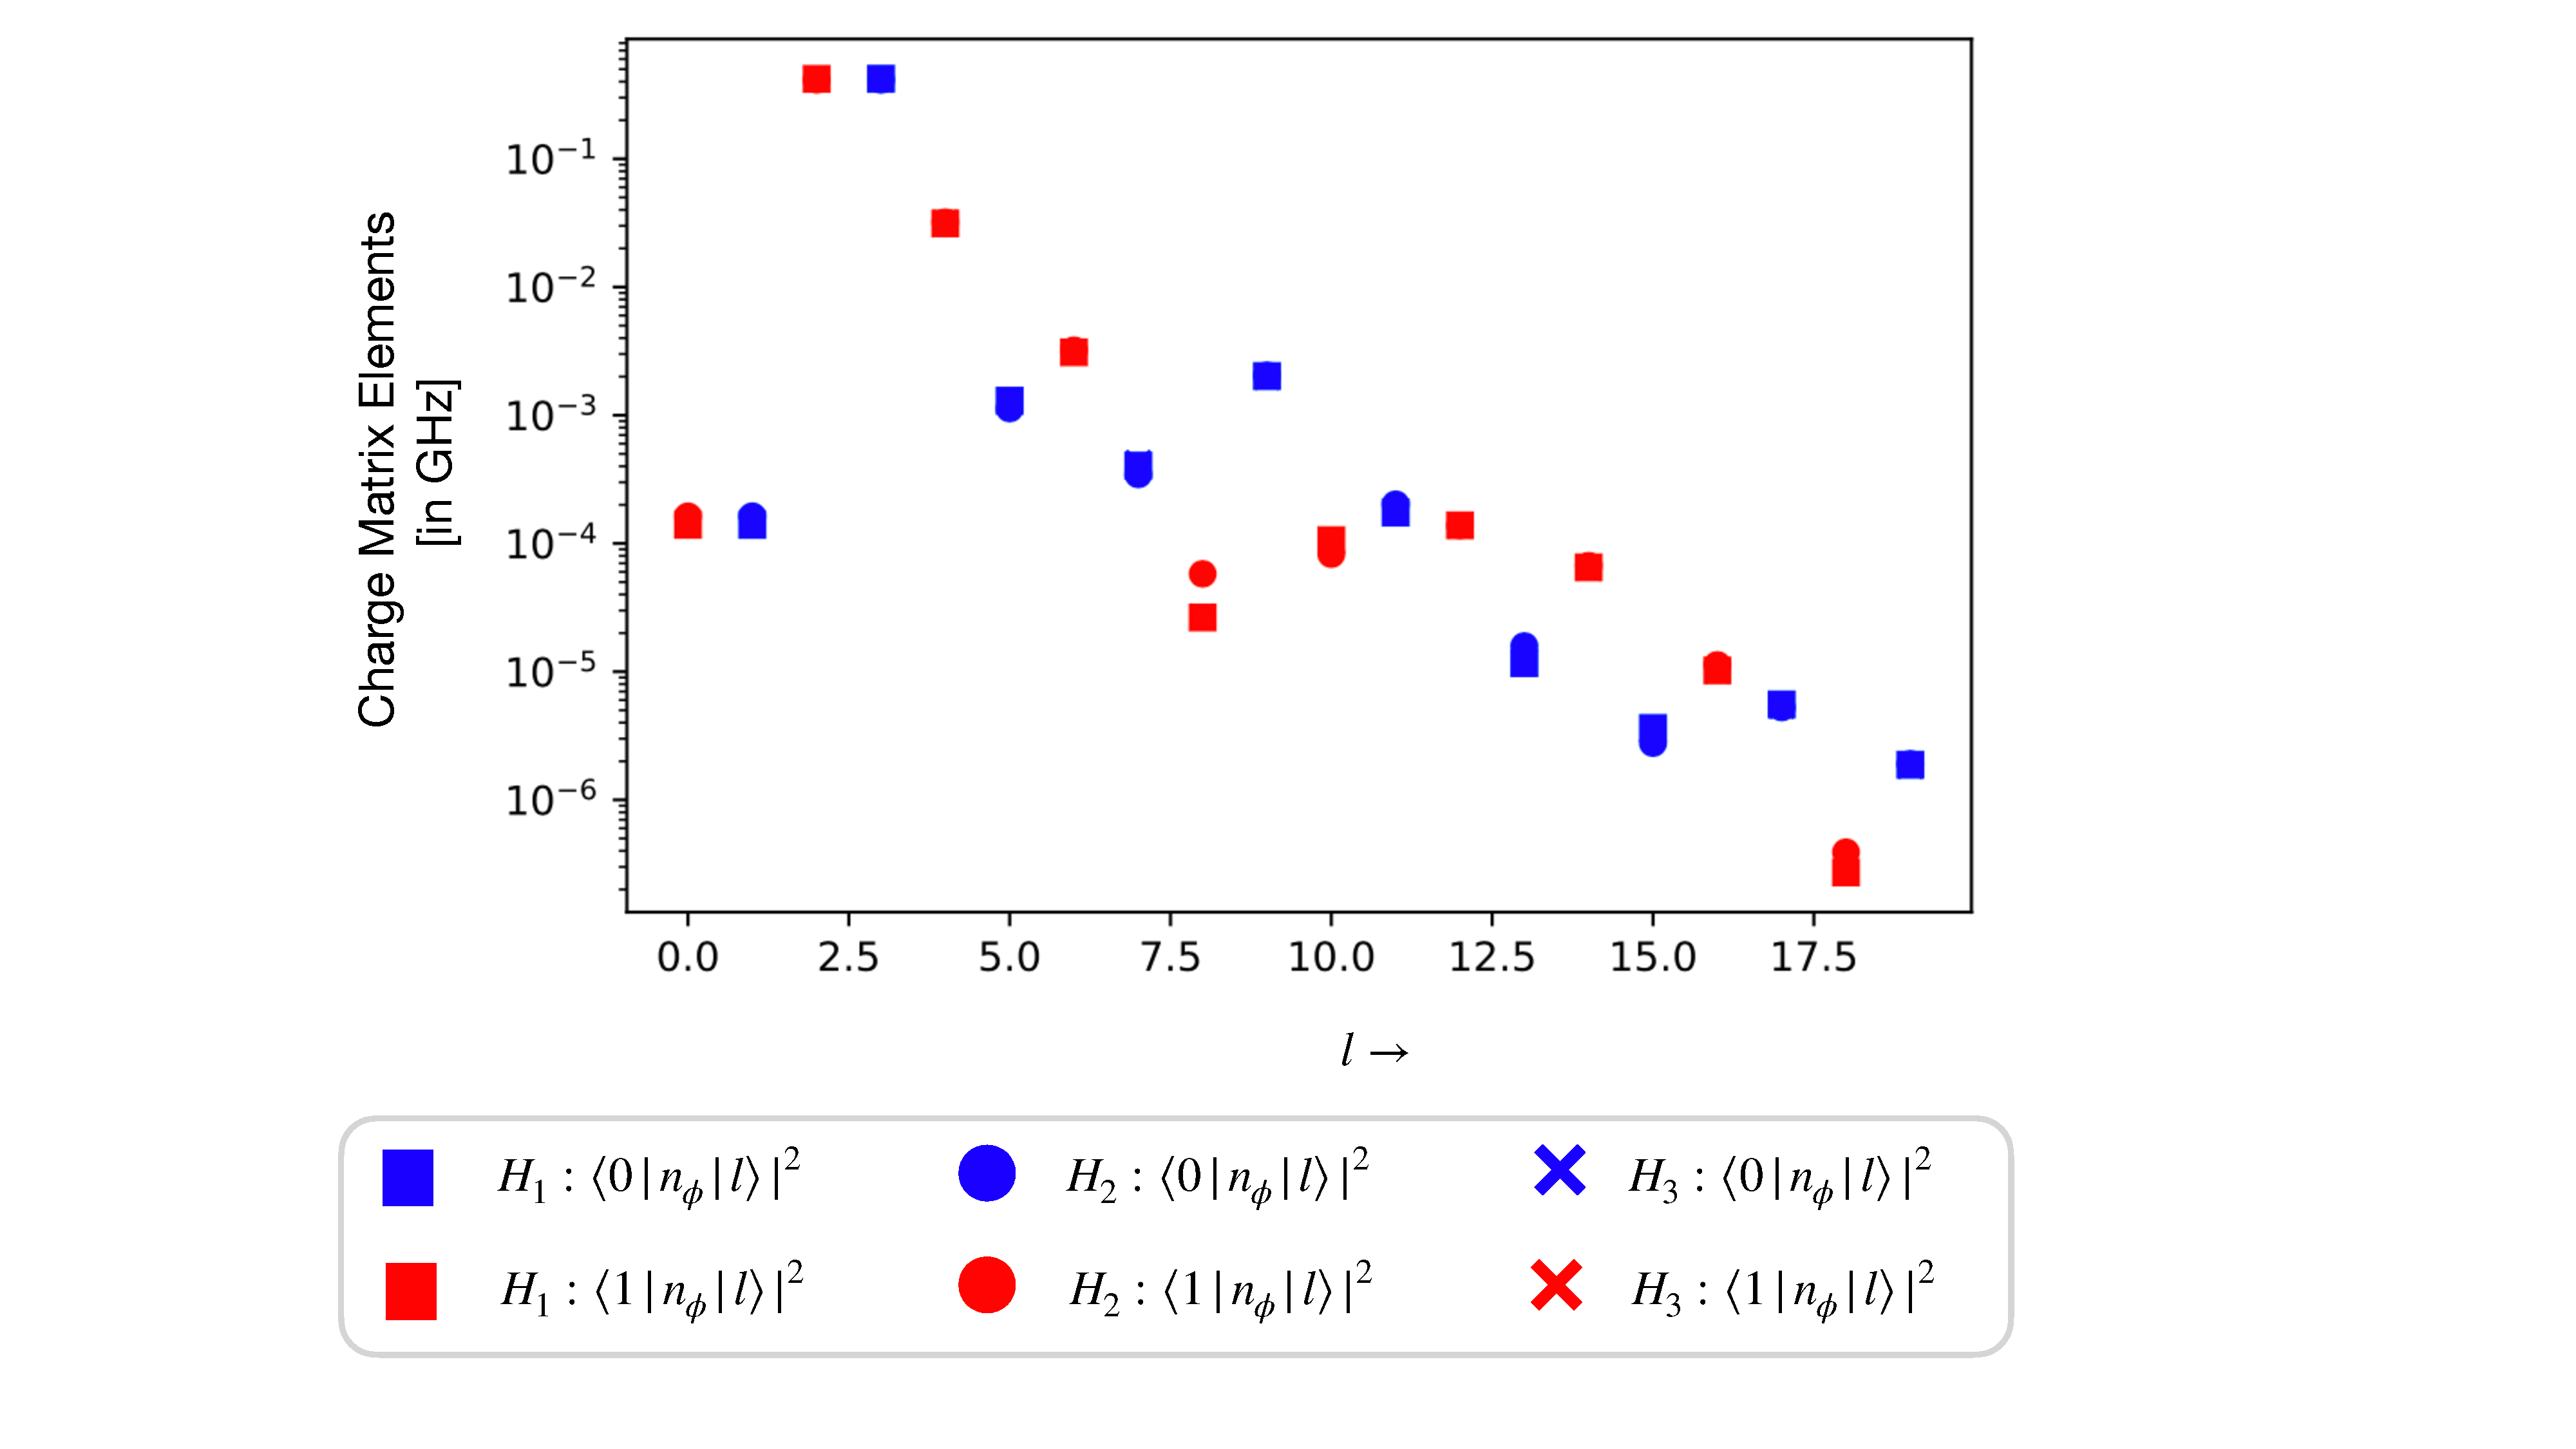
\includegraphics[width=0.45\textwidth]{Figures/Charge_Matrix.pdf}
    \caption{Charge Matrix Elements (squared) for all three circuits. Note that in the equations below we substitute $\langle l|n|l'\rangle=in_{ZPF}\langle l|a-a^\dagger|l'\rangle$ where $n_{ZPF}=\frac{1}{\sqrt{2}}\Big(E_{J,j}/8NE_C\Big)^{1/4}$. The charge matrix elements between odd-odd or even-even is zero (points not seen in log plot) due to the symmetry of cosine potential at $\varphi_\mathrm{ext}=0.5\Phi_0$, where $\Phi_0$ is the flux quantum.}
    \label{charge-matrix}
\end{figure}


\paragraph{Coupling Constant Landscape:}
The coupling constants decrease with increasing $\mu$. We plot the coupling constants for the parallel circuit named $H_1$ in Fig.~\ref{fig:meas_circuit} of the main text in Fig.~\ref{fig:coupling-strength}. In addition, we give coupling constants of the single-point connection circuits, elaborated in Sec.~\ref{app:alt_circuits}.
\begin{figure}[htb]
    \centering
    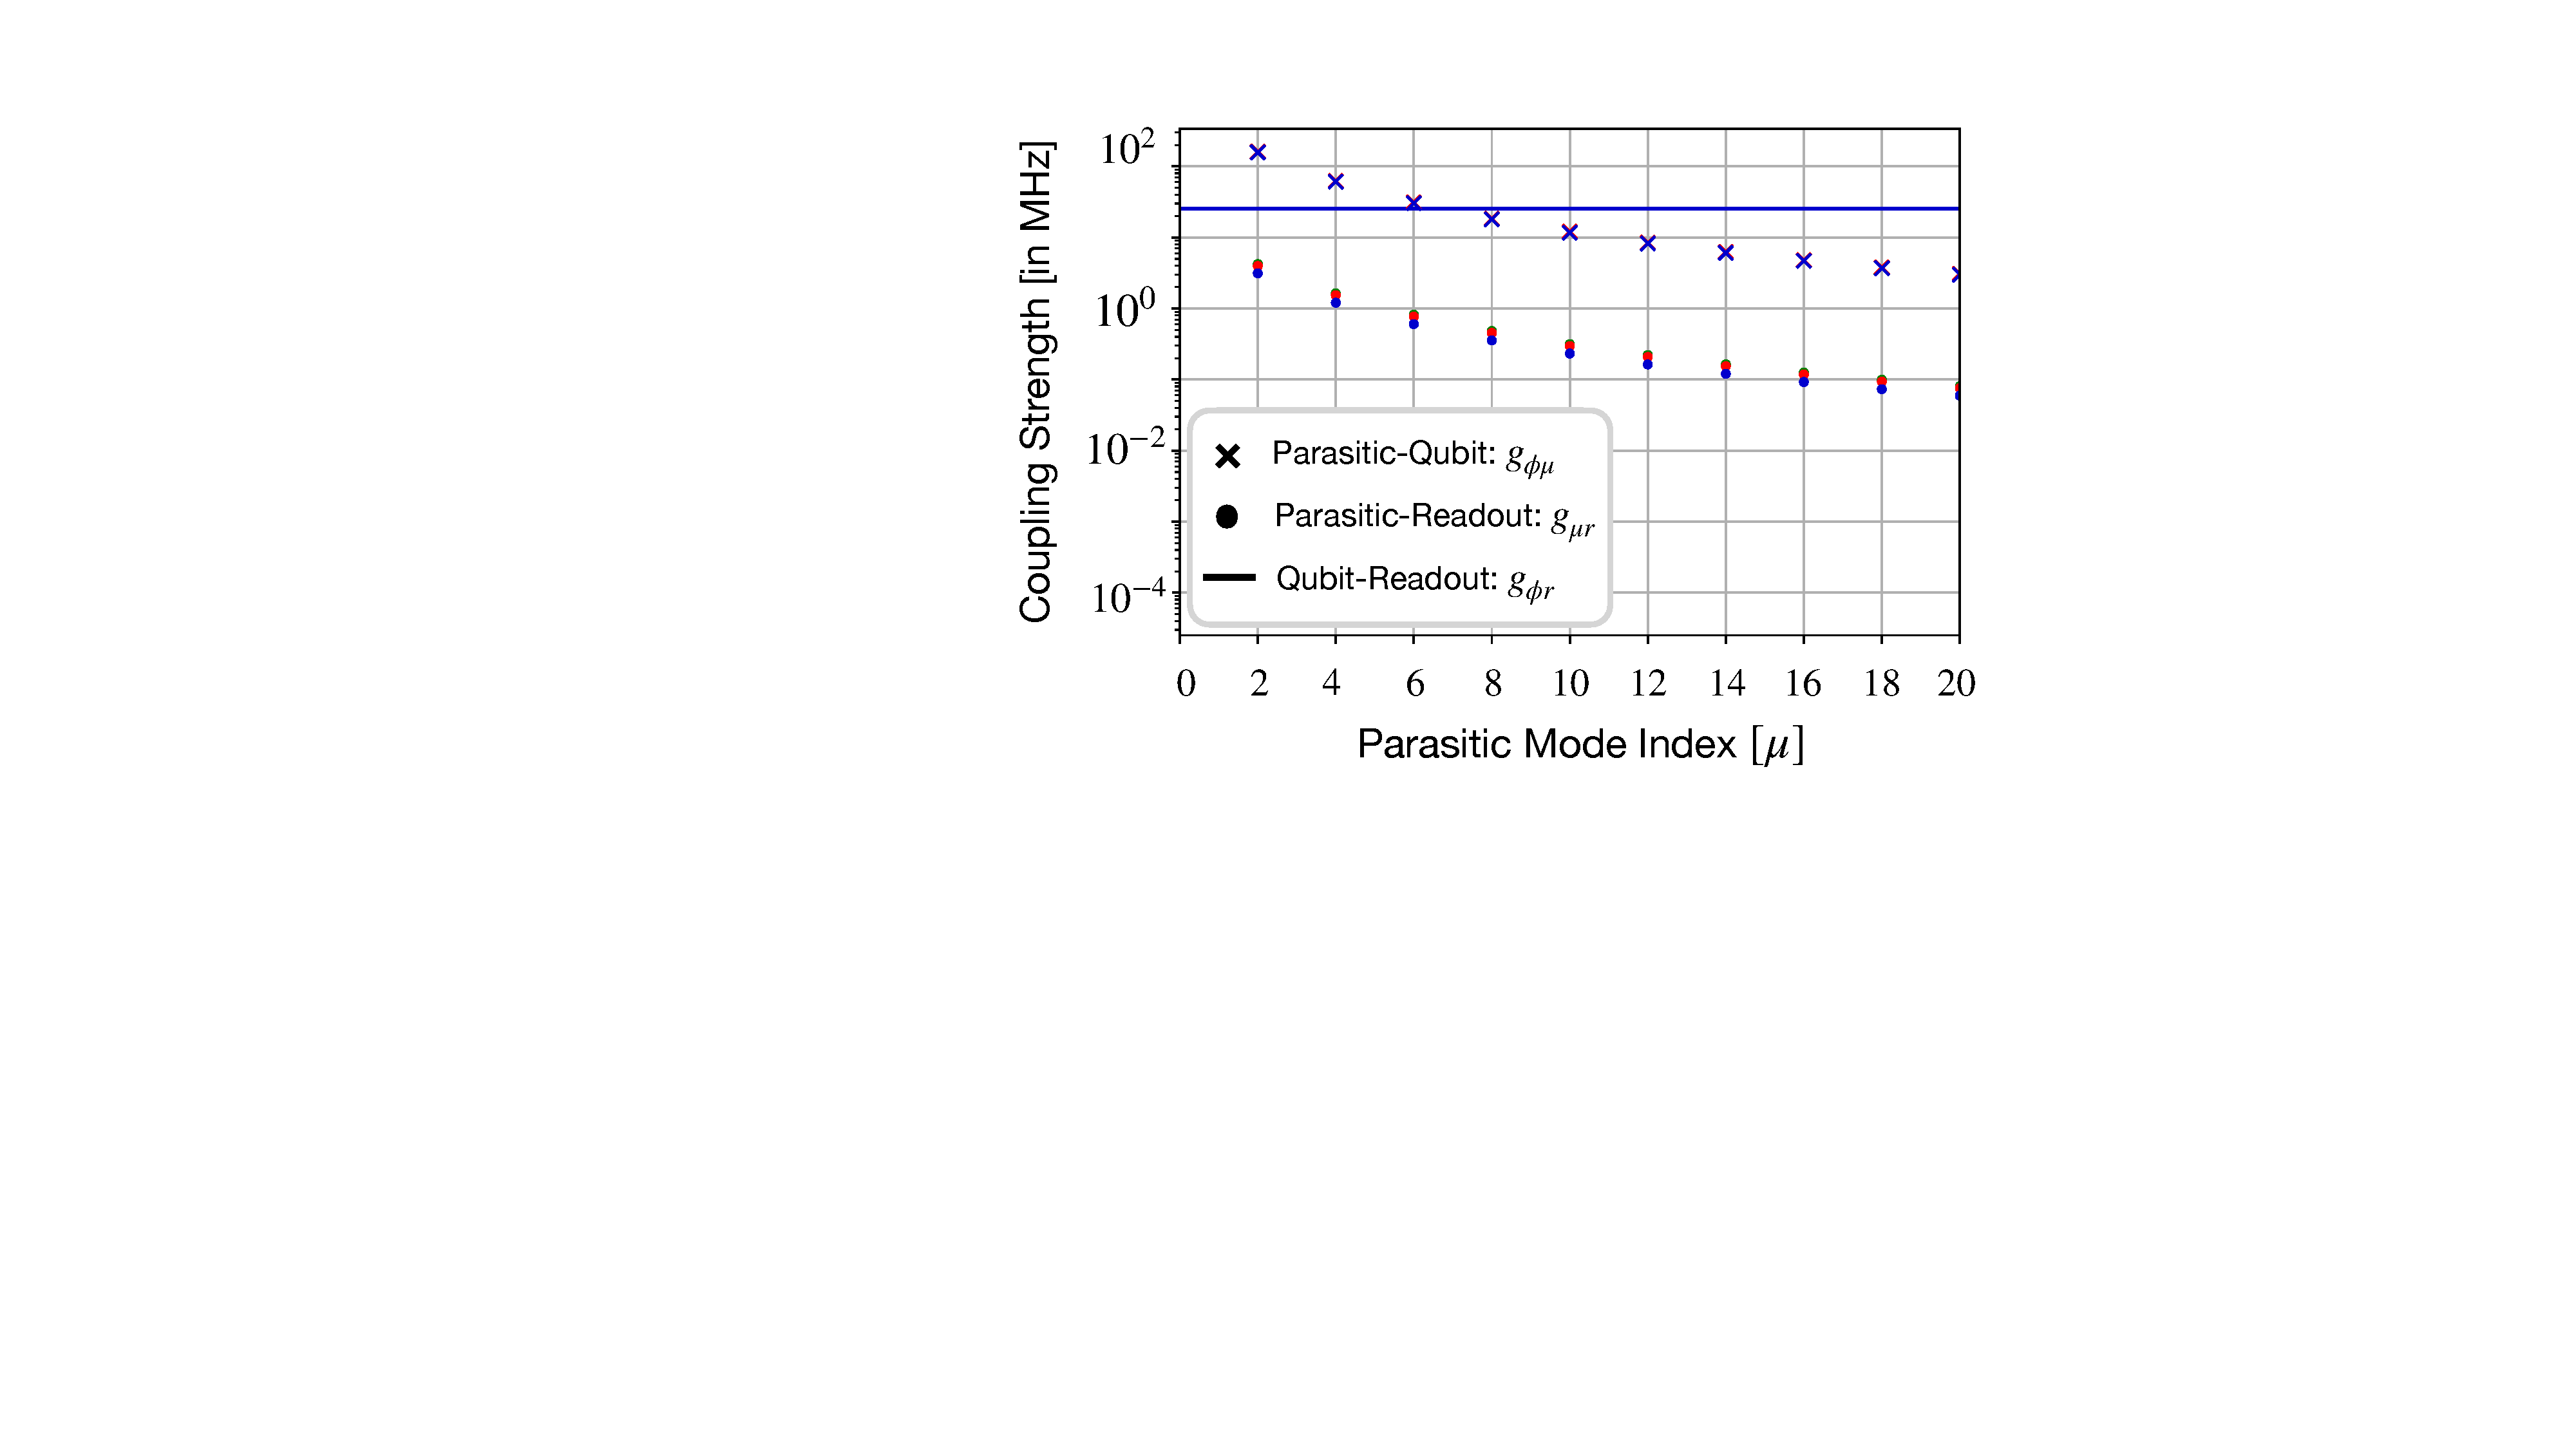
\includegraphics[width=\linewidth]{Figures/Coupling_strength.pdf}
    \caption{Absolute values of the coupling strengths in GHz for various circuits. $H_1$ (green): Parallel circuit (see Fig.~\ref{fig:meas_circuit}), $H_2$ (blue): single-Point connection with floating fluxonium  (see Fig.~\ref{fig:circuit_choice} (b)), and $H_3$ (red): single-Point Connection with grounded fluxonium (see Fig.~\ref{fig:circuit_choice} (c)). The behavior for all circuits is the same, thus the discussion in the main text focused on $H_1$ can be easily extended to $H_2,H_3$. Coupling to odd parasitic modes is zero due to the symmetries of the circuit~\cite{viola2015collective}.}
    \label{fig:coupling-strength}
\end{figure}

Below in Fig.~\ref{fig:circuit_comp} is the dependence of charging energies and coupling constants on the number of junctions as well as the ground capacitance.
\begin{figure}
    \centering
    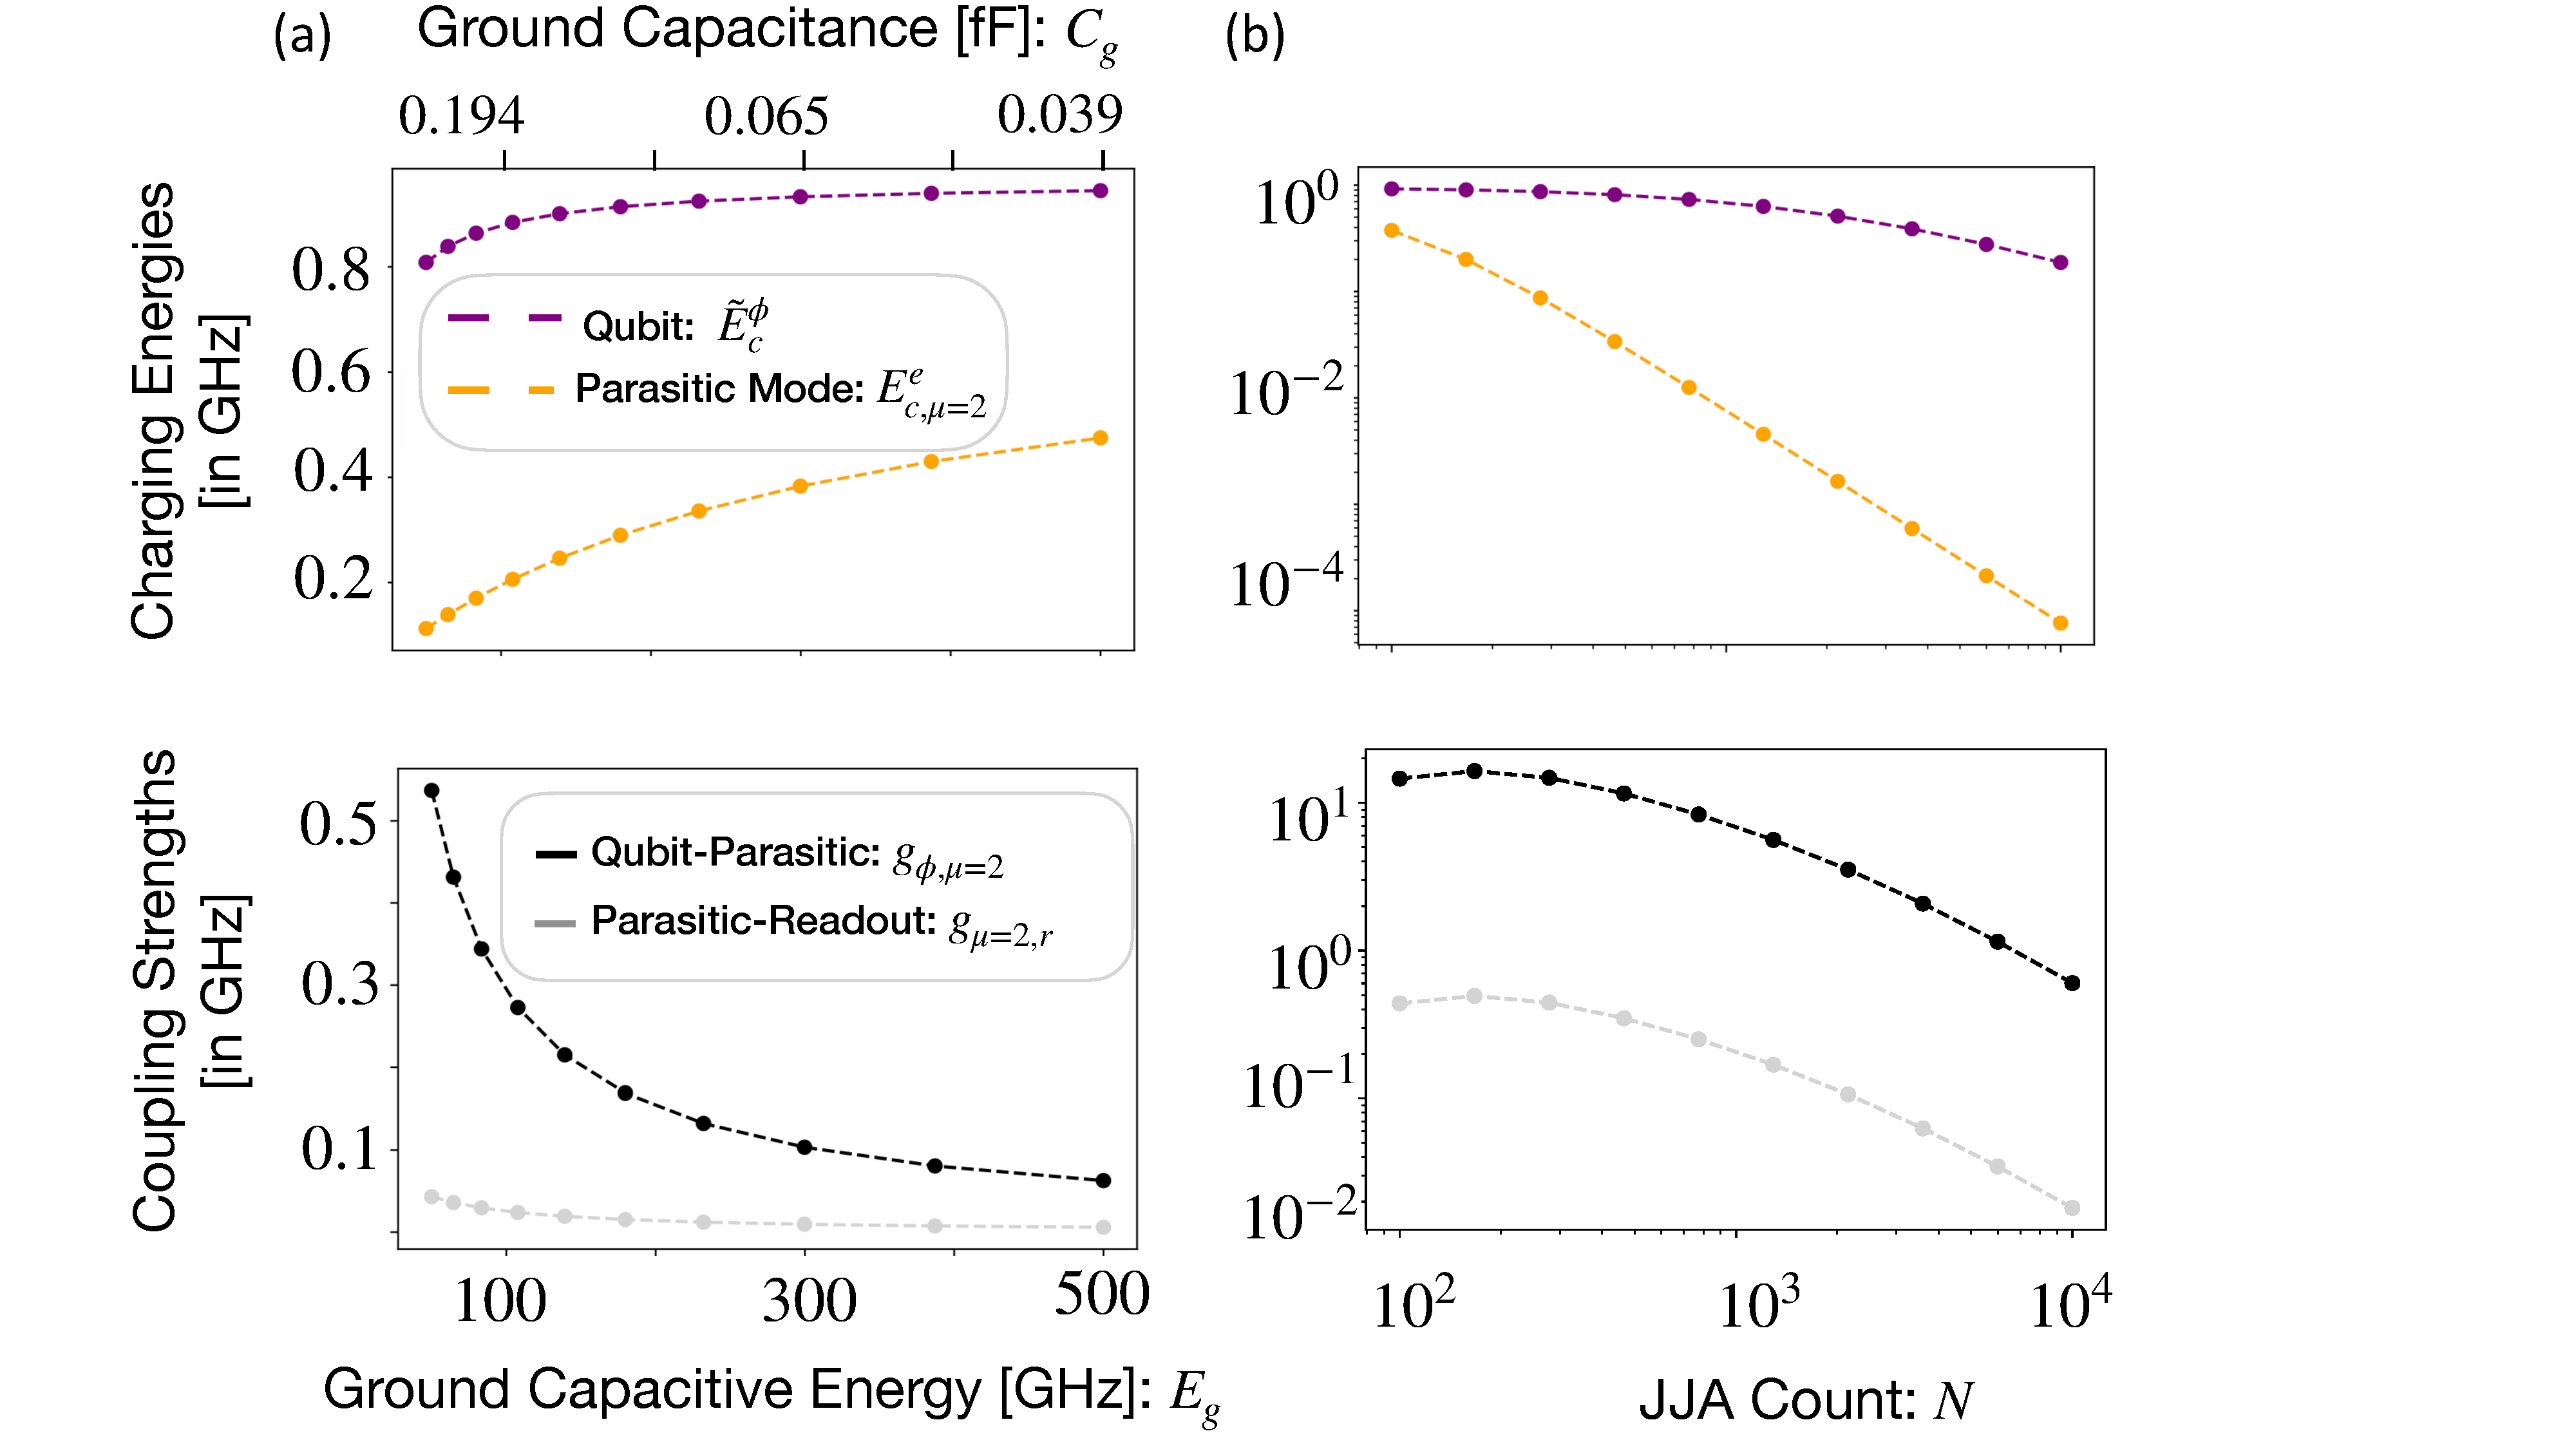
\includegraphics[width=\linewidth]{Figures/circuit_comp.pdf}
    \caption{The qubit charging energy in (a) decides the frequency and the parasitic charging energy in (b) decides the parasitic mode frequency. (c,d) give the plots for the coupling strengths of the parasitic mode to readout and qubit, respectively. All plots are obtained under linear JJA approximation. \sh{Add factor $1/2\pi$ for the coupling strengths notations in the legend. Correct these plots}}
    \label{fig:circuit_comp}
\end{figure}

\subsection{Dispersive Hamiltonian}
We use the Schrieffer-Wolff approximation to extract the readout parameters in Table.~\ref{tab:readout_params}, for example, dispersive shift of the qubit due to the parasitic modes $\chi_{\phi\mu}$ and the readout mode $\chi_{\phi r}$~\cite{viola2015collective} used to generate Fig.~\ref{fig:dephasing}, 
\allowdisplaybreaks{
\begin{align}
    2\pi H&=\frac{\omega_q}{2}\sigma_z+\sum_{\mu}(\omega_\mu+k_\mu) a_\mu^\dagger a_\mu
    +\omega_r a_r^\dagger a_r\nonumber\\ &\quad +\chi_{r,\phi}\sigma_z a_r^\dagger a_r
    +\sum_{\mu}\chi_{\mu,\phi}\sigma_z a_\mu^\dagger a_\mu
   \nonumber\\&\quad +\sum_{\mu}\chi_{r\mu} a_\mu^\dagger a_\mu a_r^\dagger a_r\\
   &=\frac{\omega_q}{2}\sigma_z+\Big(\omega_r +\chi_{r\phi}\sigma_z\Big)a_r^\dagger a_r\nonumber\\&+\sum_{\mu}\Big(\omega_\mu+k_\mu+\chi_{r\mu}a_r^\dagger a_r+\chi_{\mu\phi}\sigma_z\Big) a_\mu^\dagger a_\mu\label{eq:dispersive}
    \\
    &\text{where}\quad\omega_q\text{ or }\omega_{01}=\epsilon_0-\epsilon_1\nonumber\\ &+|\langle 0|p_\phi|1\rangle|^2\Bigg[16g_{r\phi}^2E_{C_r}^2\sqrt{\frac{E_{L_r}}{32E_{C_r}}}\frac{2\epsilon_{01}}{\epsilon_{01}^2-\omega_r^2}\nonumber\\ &\quad+\sum_\mu\Bigg\{g_{\mu\phi}^2\sqrt{\frac{E_J^j}{32\tilde{E}_{C,\mu}^e}}\frac{2\epsilon_{01}}{\epsilon_{01}^2-\omega_\mu^2}\Bigg\}\Bigg]\nonumber\\&+\sum_{l>1}16g_{r\phi}^2E_{C_r}^2\sqrt{\frac{E_{L_r}}{32E_{C_r}}}\Bigg[\frac{|\langle 0|p_\phi|l\rangle|^2}{\epsilon_{0l}-\omega_r}\nonumber\\&-\frac{|\langle 1|p_\phi|l\rangle|^2}{\epsilon_{1l}-\omega_r}\Bigg]+\sum_{l>1,\mu}\Bigg\{g_{\mu\phi}^2\sqrt{\frac{E_J^j}{32\tilde{E}_{C,\mu}^e}}\times\nonumber \\&\quad\Bigg[\frac{|\langle 0|p_\phi|l\rangle|^2}{\epsilon_{0l}-\omega_\mu}-\frac{|\langle 1|p_\phi|l\rangle|^2}{\epsilon_{1l}-\omega_\mu}\Bigg]\Bigg\}\\
   k_{\mu\in 2\mathbb{Z}}&=16E_{C_r}^2\sqrt{\frac{E_{L_r}}{32E_{C_r}}}\sqrt{\frac{E_J^j}{32E_C^e}}\Bigg[\frac{g_{r\mu}^2}{\omega_\mu-\omega_r}\Bigg]\nonumber\\&\quad\le\mathcal{O}(10^{-8})\\
\chi_{r,\phi}&=16g_{r\phi}^2E_{C_r}^2\sqrt{\frac{E_{L_r}}{32E_{C_r}}}\frac{2\epsilon_{01}}{\epsilon_{01}^2-\omega_r^2}|\langle 0|p_\phi|1 \rangle|^2\nonumber\\
   &+16g_{r\phi}^2E_{C_r}^2\sqrt{\frac{E_{L_r}}{32E_{C_r}}}\Bigg[\sum_l|\langle 0|p_\phi|l \rangle|^2\frac{\epsilon_{0l}}{\epsilon_{0l}^2-\omega_r^2}\nonumber\\&\quad-\sum_l|\langle 1|p_\phi|l \rangle|^2\frac{\epsilon_{1l}}{\epsilon_{1l}^2-\omega_r^2}\Bigg] \\
   \chi_{\mu,\phi}&=g_{\mu\phi}^2\sqrt{\frac{E_J^j}{32\tilde{E}_{C,\mu}^e}}\frac{2\epsilon_{01}}{\epsilon_{01}^2-\omega_\mu^2}|\langle 0|p_\phi|1 \rangle|^2\nonumber\\
   &+g_{\mu\phi}^2\sqrt{\frac{E_J^j}{32\tilde{E}_{C,\mu}^e}}\Bigg[\sum_l|\langle 0|p_\phi|l \rangle|^2\frac{\epsilon_{0l}}{\epsilon_{0l}^2-\omega_\mu^2}\nonumber\\&\quad-\sum_l|\langle 1|p_\phi|l \rangle|^2\frac{\epsilon_{1l}}{\epsilon_{1l}^2-\omega_\mu^2}\Bigg]
   \quad\text{(see Fig.~\ref{fig:dispersive-shift})}
\end{align}
}
Therefore $\omega_q=-7e-04 \ \mathrm{GHz}$, $\omega_{q,r}=-1.1e-03 \ \mathrm{GHz}$, see Fig.~\ref{fig:dispersive-shift} for $\omega_{q,\mu},\chi_{\mu,\phi}$.
   
The dispersive shift between the qubit and the readout is small due to the small charge matrix elements. The primary element which contributes to this quantity is the $03$ and $12$ charge matrix elements. 
\begin{figure}[htb]
    \centering
    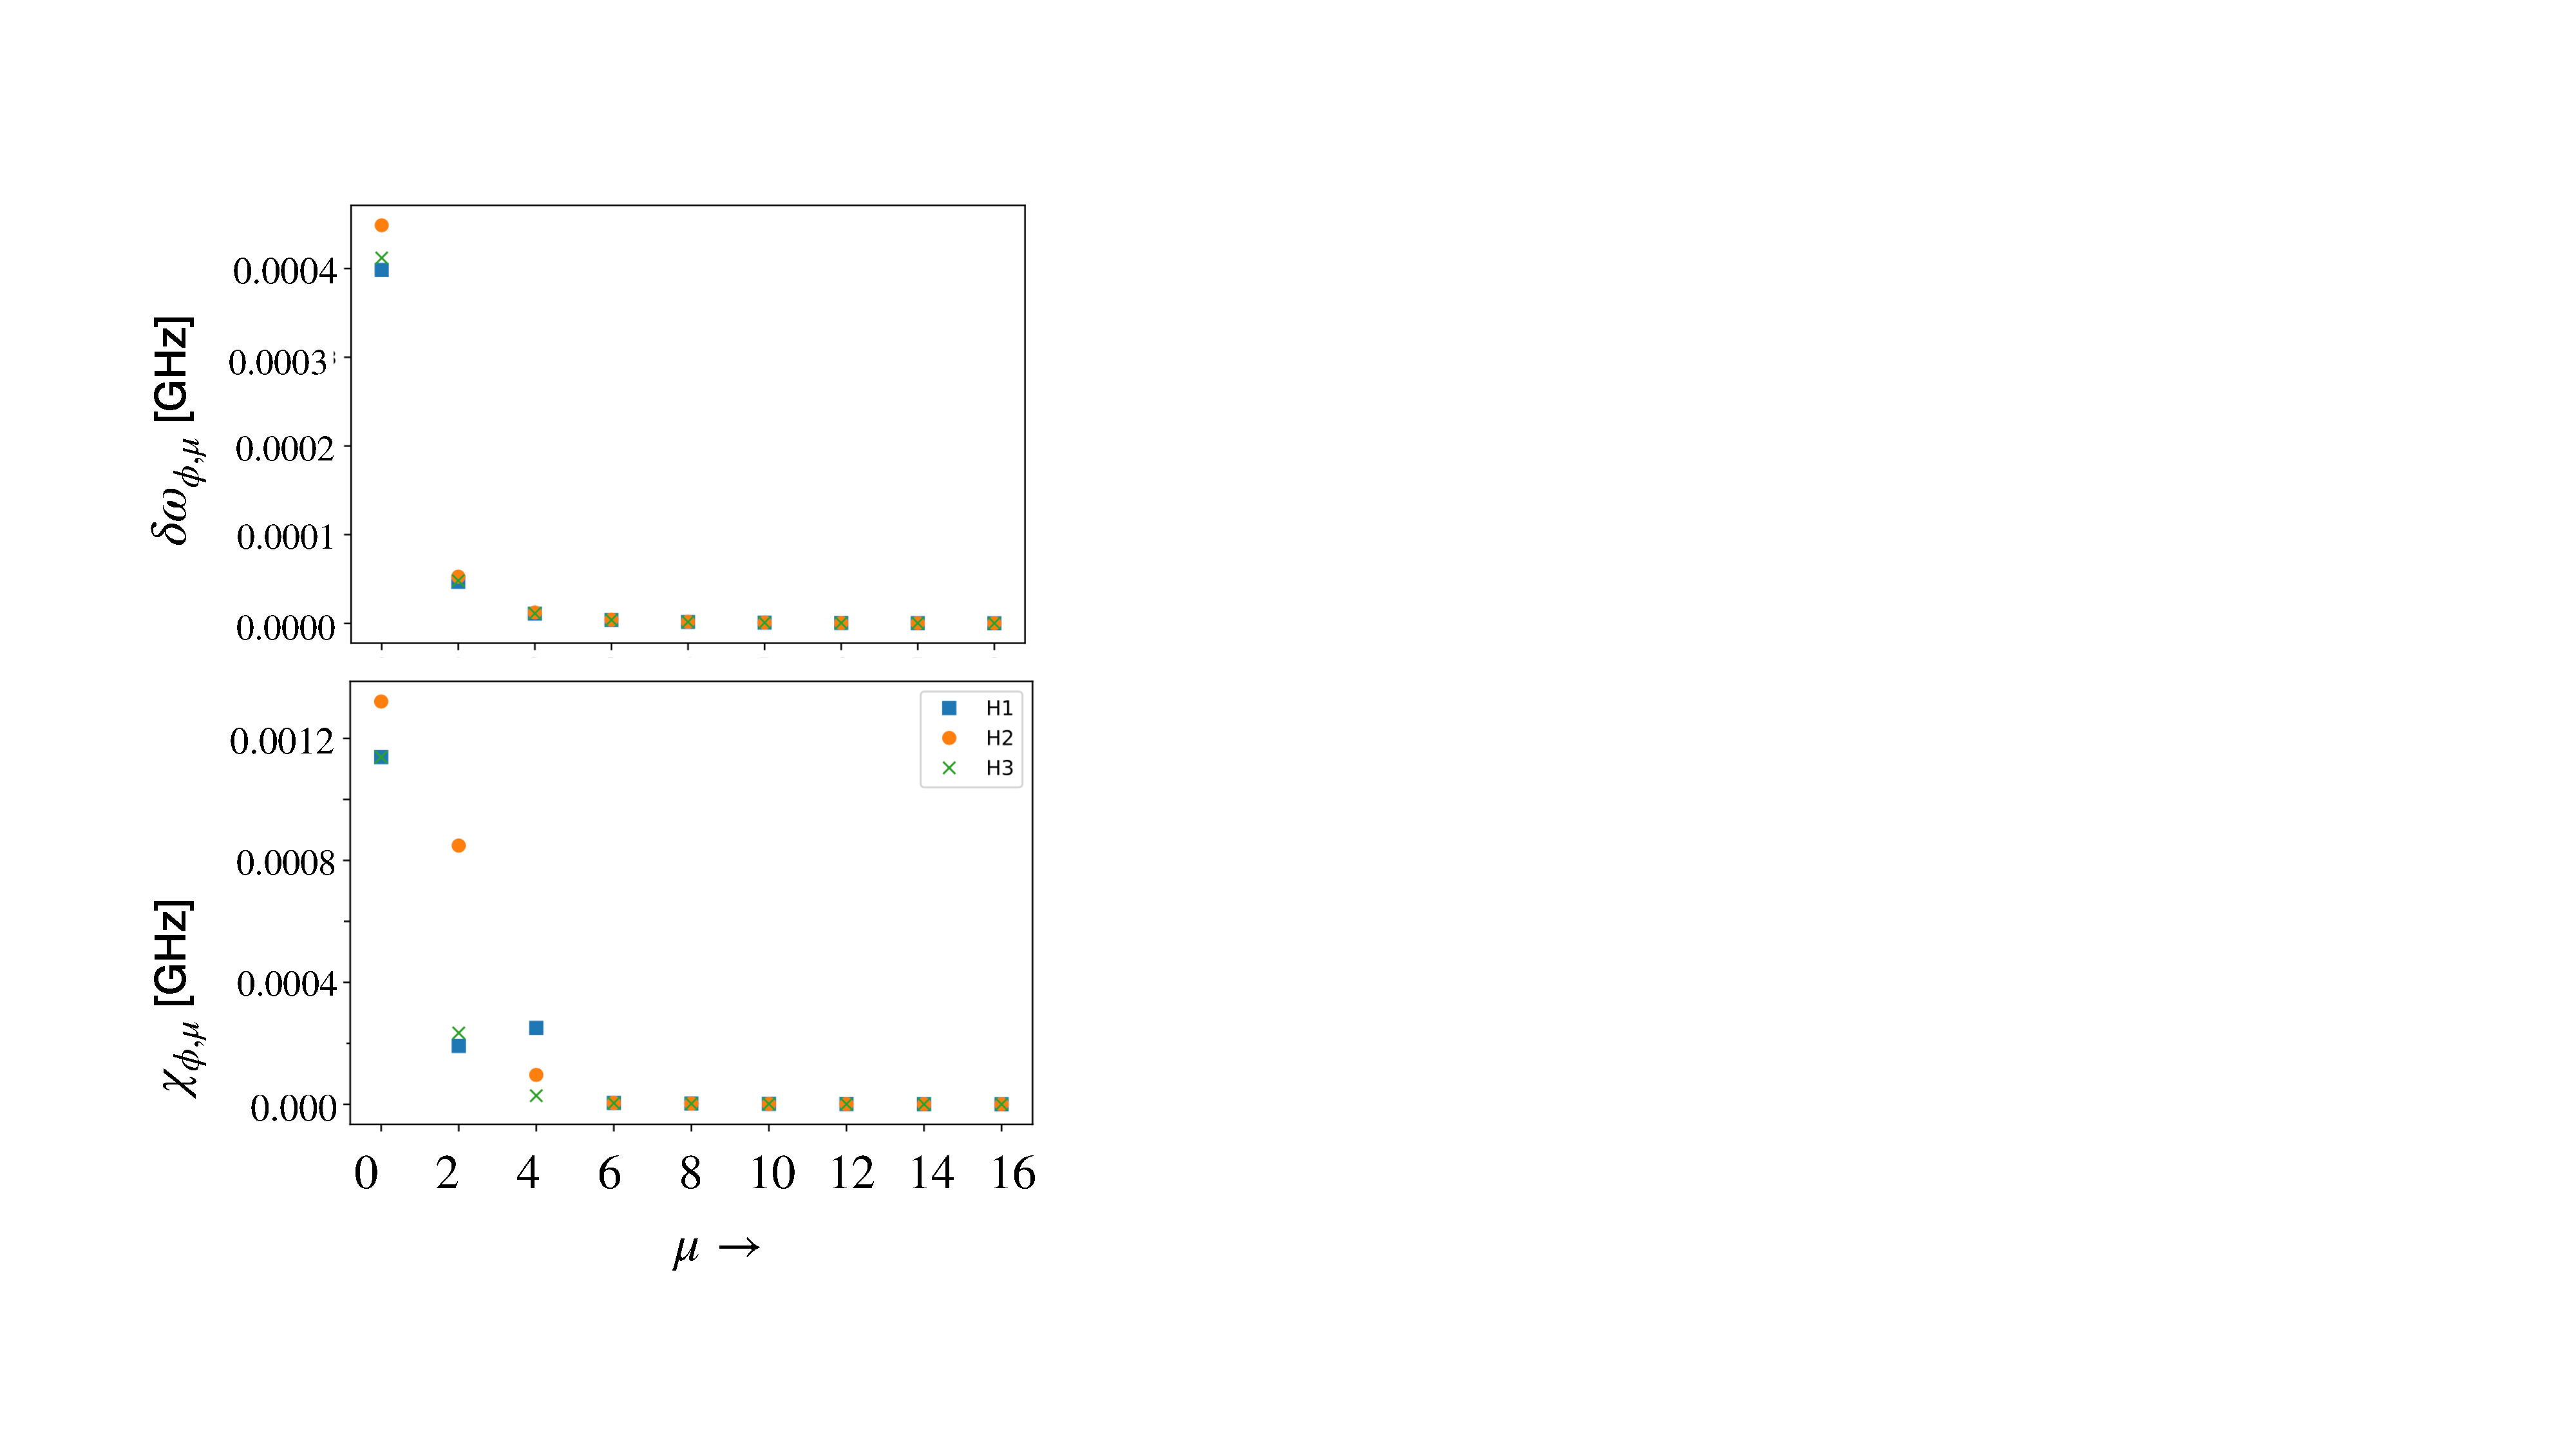
\includegraphics[width=0.45\textwidth]{Figures/dispersive-shift.pdf}
    \caption{All values are in $\frac{GHz}{2\pi}$ units. The color code follows: $H_1$ (blue), $H_2$ (orange), $H_3$ (green) for the three circuits shown in Fig.~\ref{fig:circuit_comp}(a-c). (Top) Change in the qubit frequency due to parasitic mode $\mu$ (Bottom) Dispersive shift $\chi_\mu$ of the qubit concerning the parasitic mode $\mu$.}
    \label{fig:dispersive-shift}
\end{figure}
\section{Driven Fluxonium Circuit}\label{app:MIST}
%Appendices for Sec 3
Here, we will discuss the several analyses used in the driven fluxonium circuit including the semi-classical approximation and methods used in Sec.~\ref{sec:MIST} to compute the readout efficiency. We first start with the derivation of $H_{s.c.}$ in Eq.~\ref{eq:drive}. \singh{Derivation goes here}
\subsection{Approximations for Numerical Modelling}\label{app:numerics}
We use the following three approximations to make the problem at hand simpler
\begin{itemize}
    \item Restriction to $\mu=2$. We restrict our analyses to the closest even parasitic mode that couples most strongly to the qubit and the readout as evident from Fig.~\ref{fig:circuit_comp}(d). This assumption helps us to lower bound the errors. Although it will be an interesting study to see if there are transitions caused due to higher modes that are more probable but in this work we aim at a proof of principle quantitative evidence of the presence of such transitions even with out modest assumptions.

    \item Semi-classical drive approximation. This approximation treats the readout resonator classically as described in Refs.~\cite{xiao2023diagrammatic,dumas2024unified,cohen2023reminiscence,khezri2023measurement} reducing one mode from our numerical simulation. This assumption is essential since unlike the case of transmon or fluxonium without collective modes, with all the above approximation, a full quantum simulation of the problem will still require three modes.

    \item Linear JJA Approximation. We assume that the parasitic modes behave as linear oscillators due to the large $E_{J_j}/E_{C_j}=200$ ratio. This approximation is explained in App.~\ref{app:Hamiltonian}. The nonlinear corrections to our results, while essential, is beyond the scope of this work. For details on how nonlinear corrections affect different circuit parameters in play we direct the readers to Ref.~\cite{viola2015collective}. Due to this assumption, we can use a Hilbert size of $20\times 3$ where only three levels are assumed in the linear parasitic mode subspace. In the presence of nonlinearity, the Hilbert size would need to be much larger to capture the required effects. Note that for the conclusions drawn in this paper, we are only interested in the presence of p-MIST processes and do not claim to quantify how many such transitions can be present. Hence, $3$ levels in the parasitic mode are enough. In addition, we have verified that changing the truncation of the parasitic mode to $10$ levels does not change the energy spacing.
\end{itemize}
\singh{Here goes the truncation figure}

\subsection{Stark Shift}\label{app:stark-shift}
To observe a state transition the primary requirements are high charge matrix elements and low energy difference. The eigen-eniergies of the states in question are changed with an increase in the number of readout photons or, in this case, the drive strength. So, in this section, we compute the stark shifted eigen-energies which can help in the prediction of an avoided crossing, given $\bar n_r, \omega_r$ and the charge matrix elements. These stark shift formulas are used in the computing the probability of transitions using generalized Fermi's golden rule and Landau-Zener calculations. Let $\ket{i}$ be a state in the eigenspace of $H_{int}=H_\phi+H_{\mu=2}+g_{\phi\mu}\hat N_\phi\hat N_\mu$. Following derivations in App.~\ref{app:Hamiltonian} the ac stark-shift in the energy of state $\ket{i}$ at an average number of readout photons $\bar n_r$ is given by,
\begin{align}
    \chi_i(\bar n_r)=2\bar n_r\sum_{f}\omega_{if}\Big[\frac{g_{\phi r}|\braket{i|\hat N_\phi|f}|^2}{\omega_d^2-\omega_{if}^2}+\frac{g_{\mu r}|\braket{i|\hat N_\mu|f}|^2}{\omega_d^2-\omega_{if}^2}\Big]\label{eq:stark}
\end{align}
 Here $\omega_{if}=E_f-E_i$ denote the energy difference in the eigen-energies of the $\ket{i}$. The impact due to the second term as expected is much smaller than the first term, and hence $g_{\phi r}$ primarily governs this stark shift.
 \begin{figure}
     \centering
     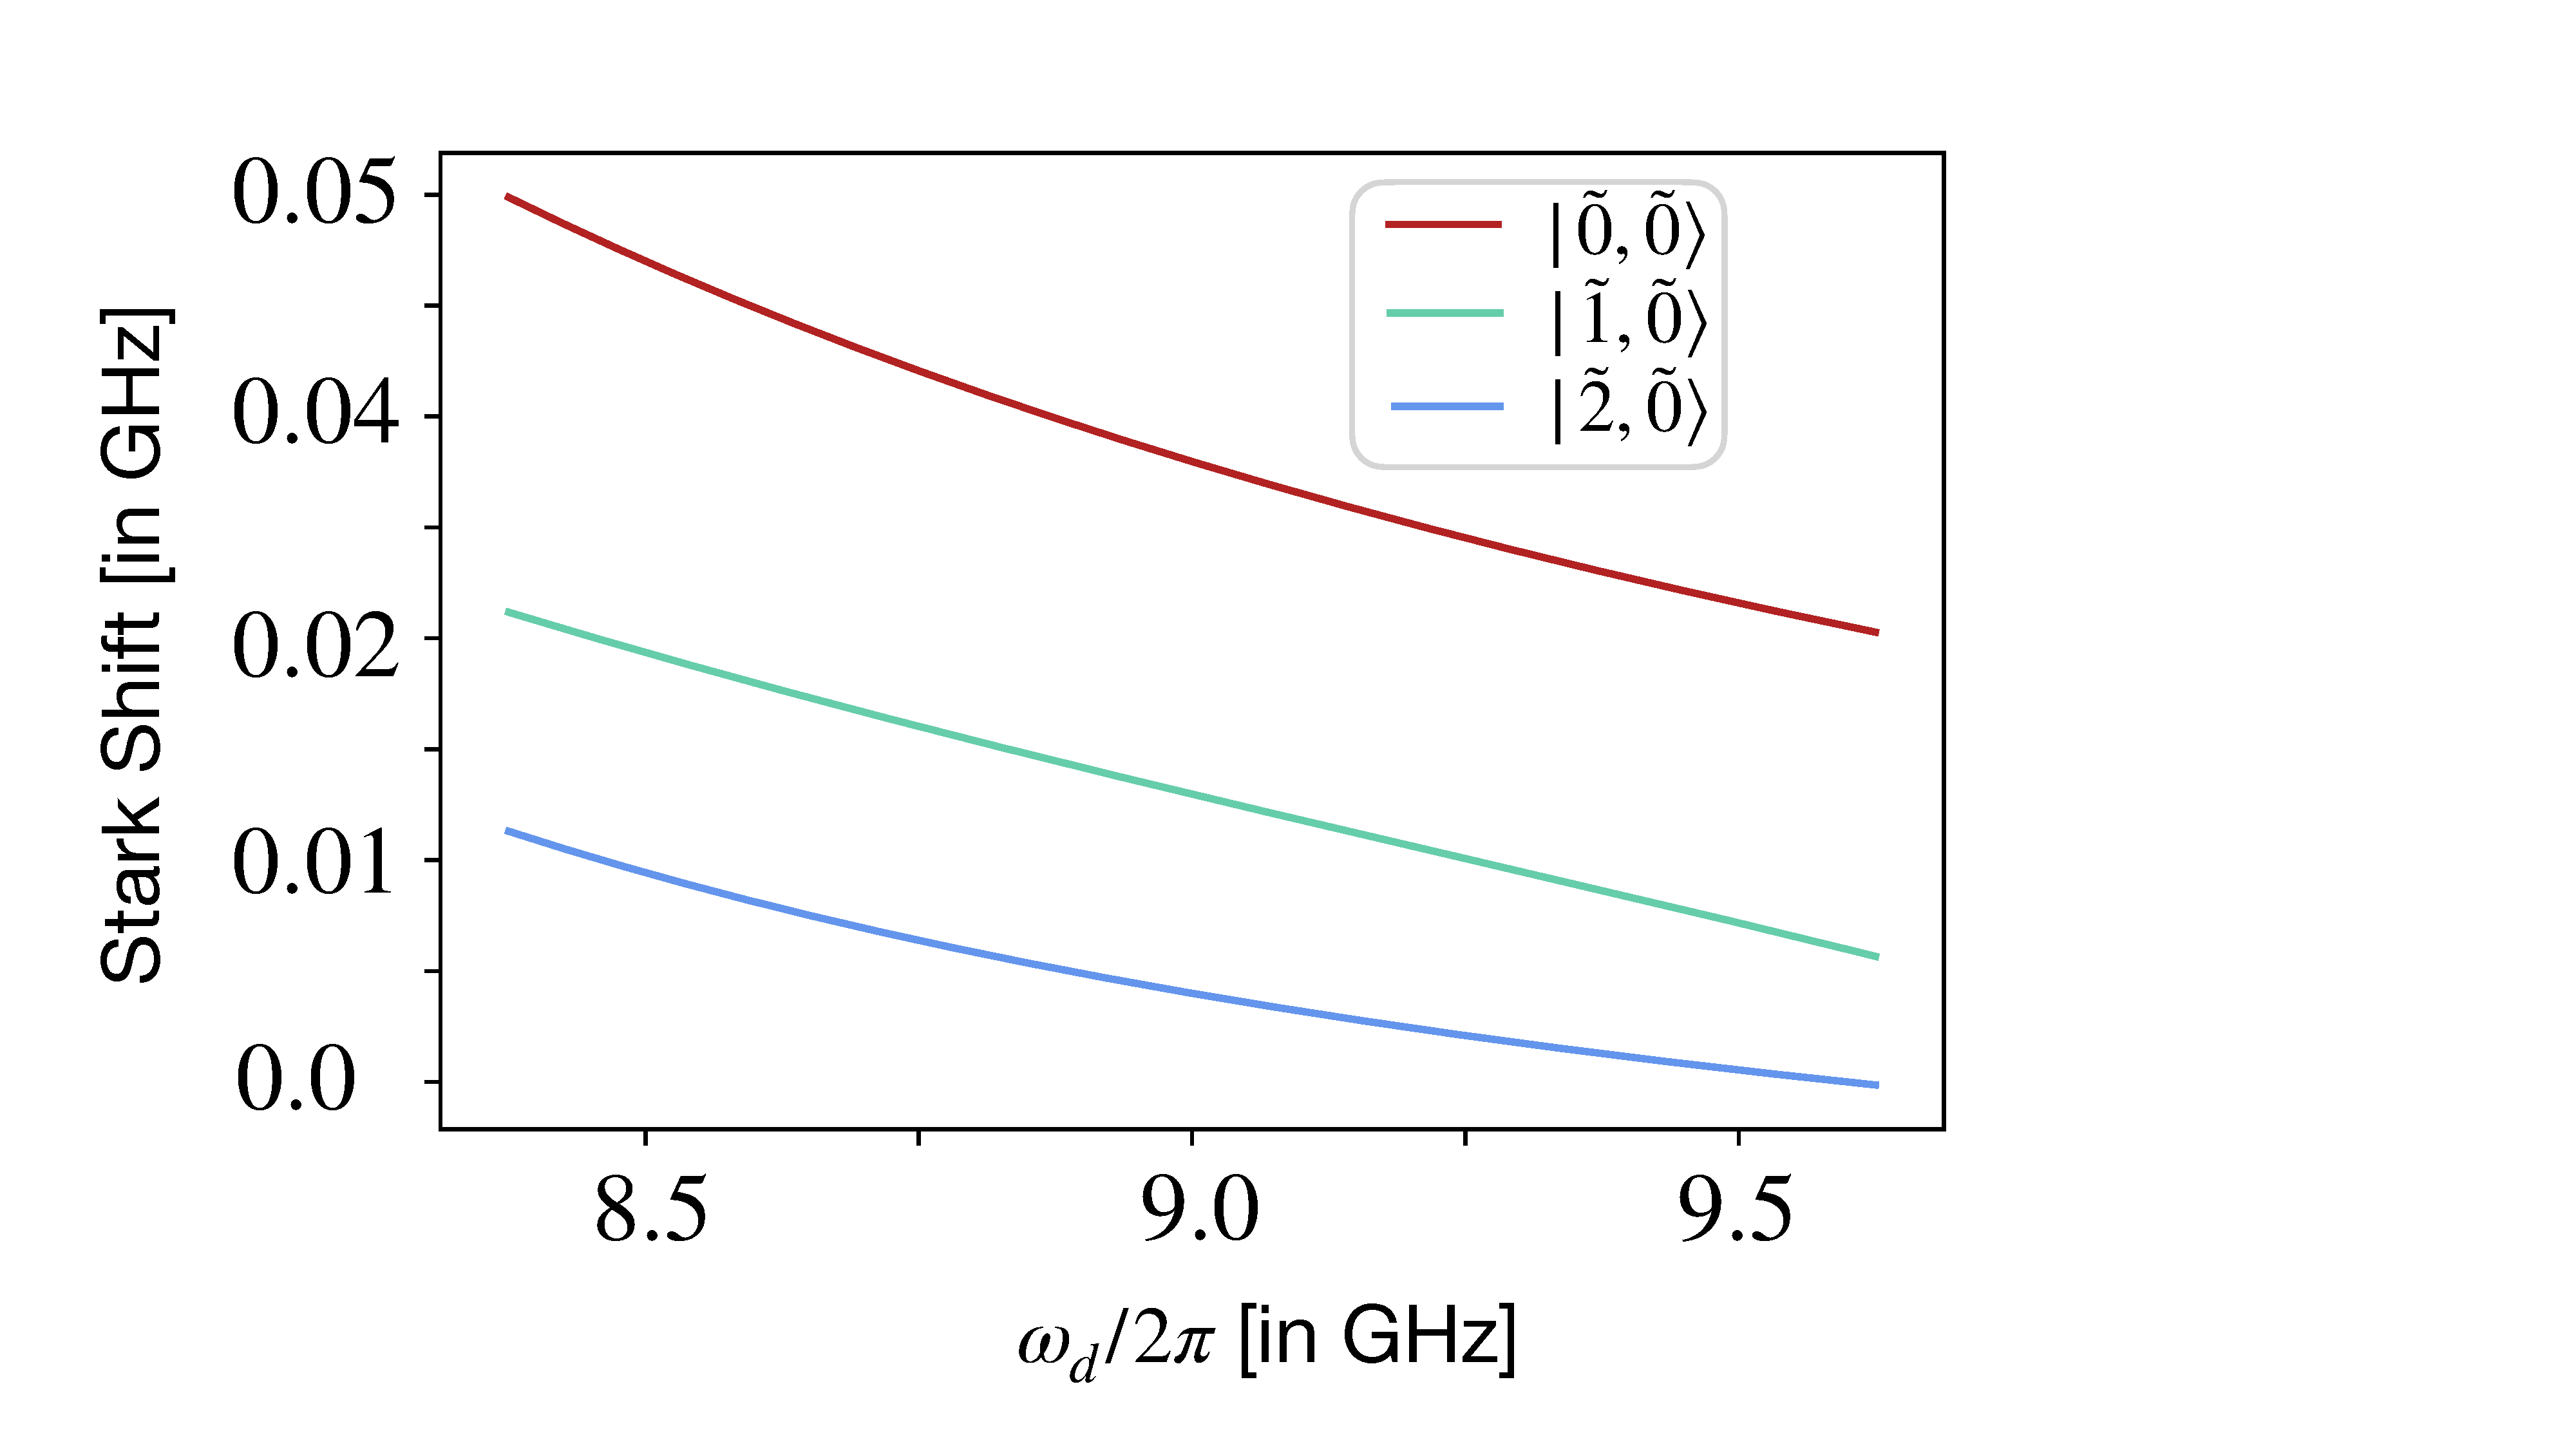
\includegraphics[width=\linewidth]{Figures/Stark-shift.pdf}
     \caption{Stark shift in different qubit levels under observation for readout computed using Eq.~\ref{eq:stark}.}
     \label{fig:stark-shift}
 \end{figure}
%\subsection{Generalized Fermi's Golden Rule}\label{app:fermi}
%We also draw our intuition from Fermi's Golden rule calculations where we have used the following formulas. Next, we will use generalized Fermi's golden rule to estimate the transition rate of the spurious excitations identified in Fig.~\ref{fig:trans_prof}, and filter out the low-rate processes that are highly probable. Here, we will use a more fine-tuned range of frequencies, and thus, we will only use a reasonable range of $\omega_d=\omega_r=[7,10] \ \mathrm{GHz}$. This choice was made to check the behavior of the circuit close to the experimentally optimized value for the readout frequency $\omega_r=8.5 \ \mathrm{GHz}$. The spacing in the frequency sweep should be of the order of $\mathcal{O}(1) \ \mathrm{MHz}$ to account for stark-shifted transition frequencies. Doing this will allow us to identify the resonant transitions without computing corrections due to stark shifts.

%Under the same classical approximation, we can identify our parent Hamiltonian as $H_0$ and perturbation $V$ as follows,
%\begin{align}
%H_0&=H_{\phi}+\omega_\mu \hat a_\mu^\dagger \hat a_\mu+g_{\phi,\mu}\hat N_\phi \hat N_\mu\\
%V&=2\sqrt{\bar n_r}(g_{r,\phi} \hat N_\phi+g_{r,\mu}\hat N_\mu)\sin{\omega_d t},
%\end{align}
%where$\mu$ is the density of states which will be a Dirac Delta function in the absence of loss while it will be Lorentzian in the presence of loss. In units of $\hbar$ we have,
%\begin{align}
%    \Gamma_{i\rightarrow f}&=|\braket{f|H_1|i}|^2\mu(E_i-E_f)\quad\textrm{(first-order)}\\
%&=\sum_m\frac{|\braket{f|H_1|m}\braket{m|H_1|i}|^2}{|E_i-E_m-2\hbar\omega_d|^2}\mu(E_f-E_i-2\hbar \omega_d)\nonumber\\&\quad\quad\quad\textrm{(second-order)}
%\end{align}
%The derivation of the last equation can be found in App.~\ref{app:fermi}. In the absence of the drive term, the term $H_{int}=g_{\phi,\mu}\hat N_\phi \hat N_\mu$ hybridizes the eigenstates of the fluxonium ($\phi$) mode and the parasitic mode ($\mu=2$). Thus, the experiment has access to the normal modes or diagonalized basis of $H_0$ and $V$ is the oscillating perturbation that causes transitions in this hybridized basis. In App.~\ref{app:fermi} we show that the hybridization changes a few states significantly. Finally, when we drive the two modes simultaneously due to the drive on the resonator, we will see that these drives will do something non-trivial on the hybridized modes. However, there exists a one-to-one mapping between the eigenstates of $H_0$ and eigenstates of the disjoint Hilbert space of the fluxonium mode and the parasitic mode. We again start in the lowest four eigenstates with $\mu=2$ and compute the transition rates using Fermi's Golden rule. We use these calculations to identify the transitions that could be observed at low photon number $(\bar n_r<100)$ using Floquet simulations. 

%For the density of states $\mu(x)$, we have two options. Since we do not include dissipation in the Floquet simulations, Fermi's golden rule results shown here are computed using Dirac-delta functions. The density of states here can be a Lorentzian to imitate a lossy cavity. 

%We plot the transition rates (in KHz) from states $\ket{0-3}$ to other levels. These hybridized states can be associated very closely with the disjoint system of fluxonium and parasitic mode. In the figure here, we marked a few transitions to identify particular instances of parasitic mode triggered p-MIST processes, as described in the main text.
%\begin{figure}[htb]
%    \centering
%    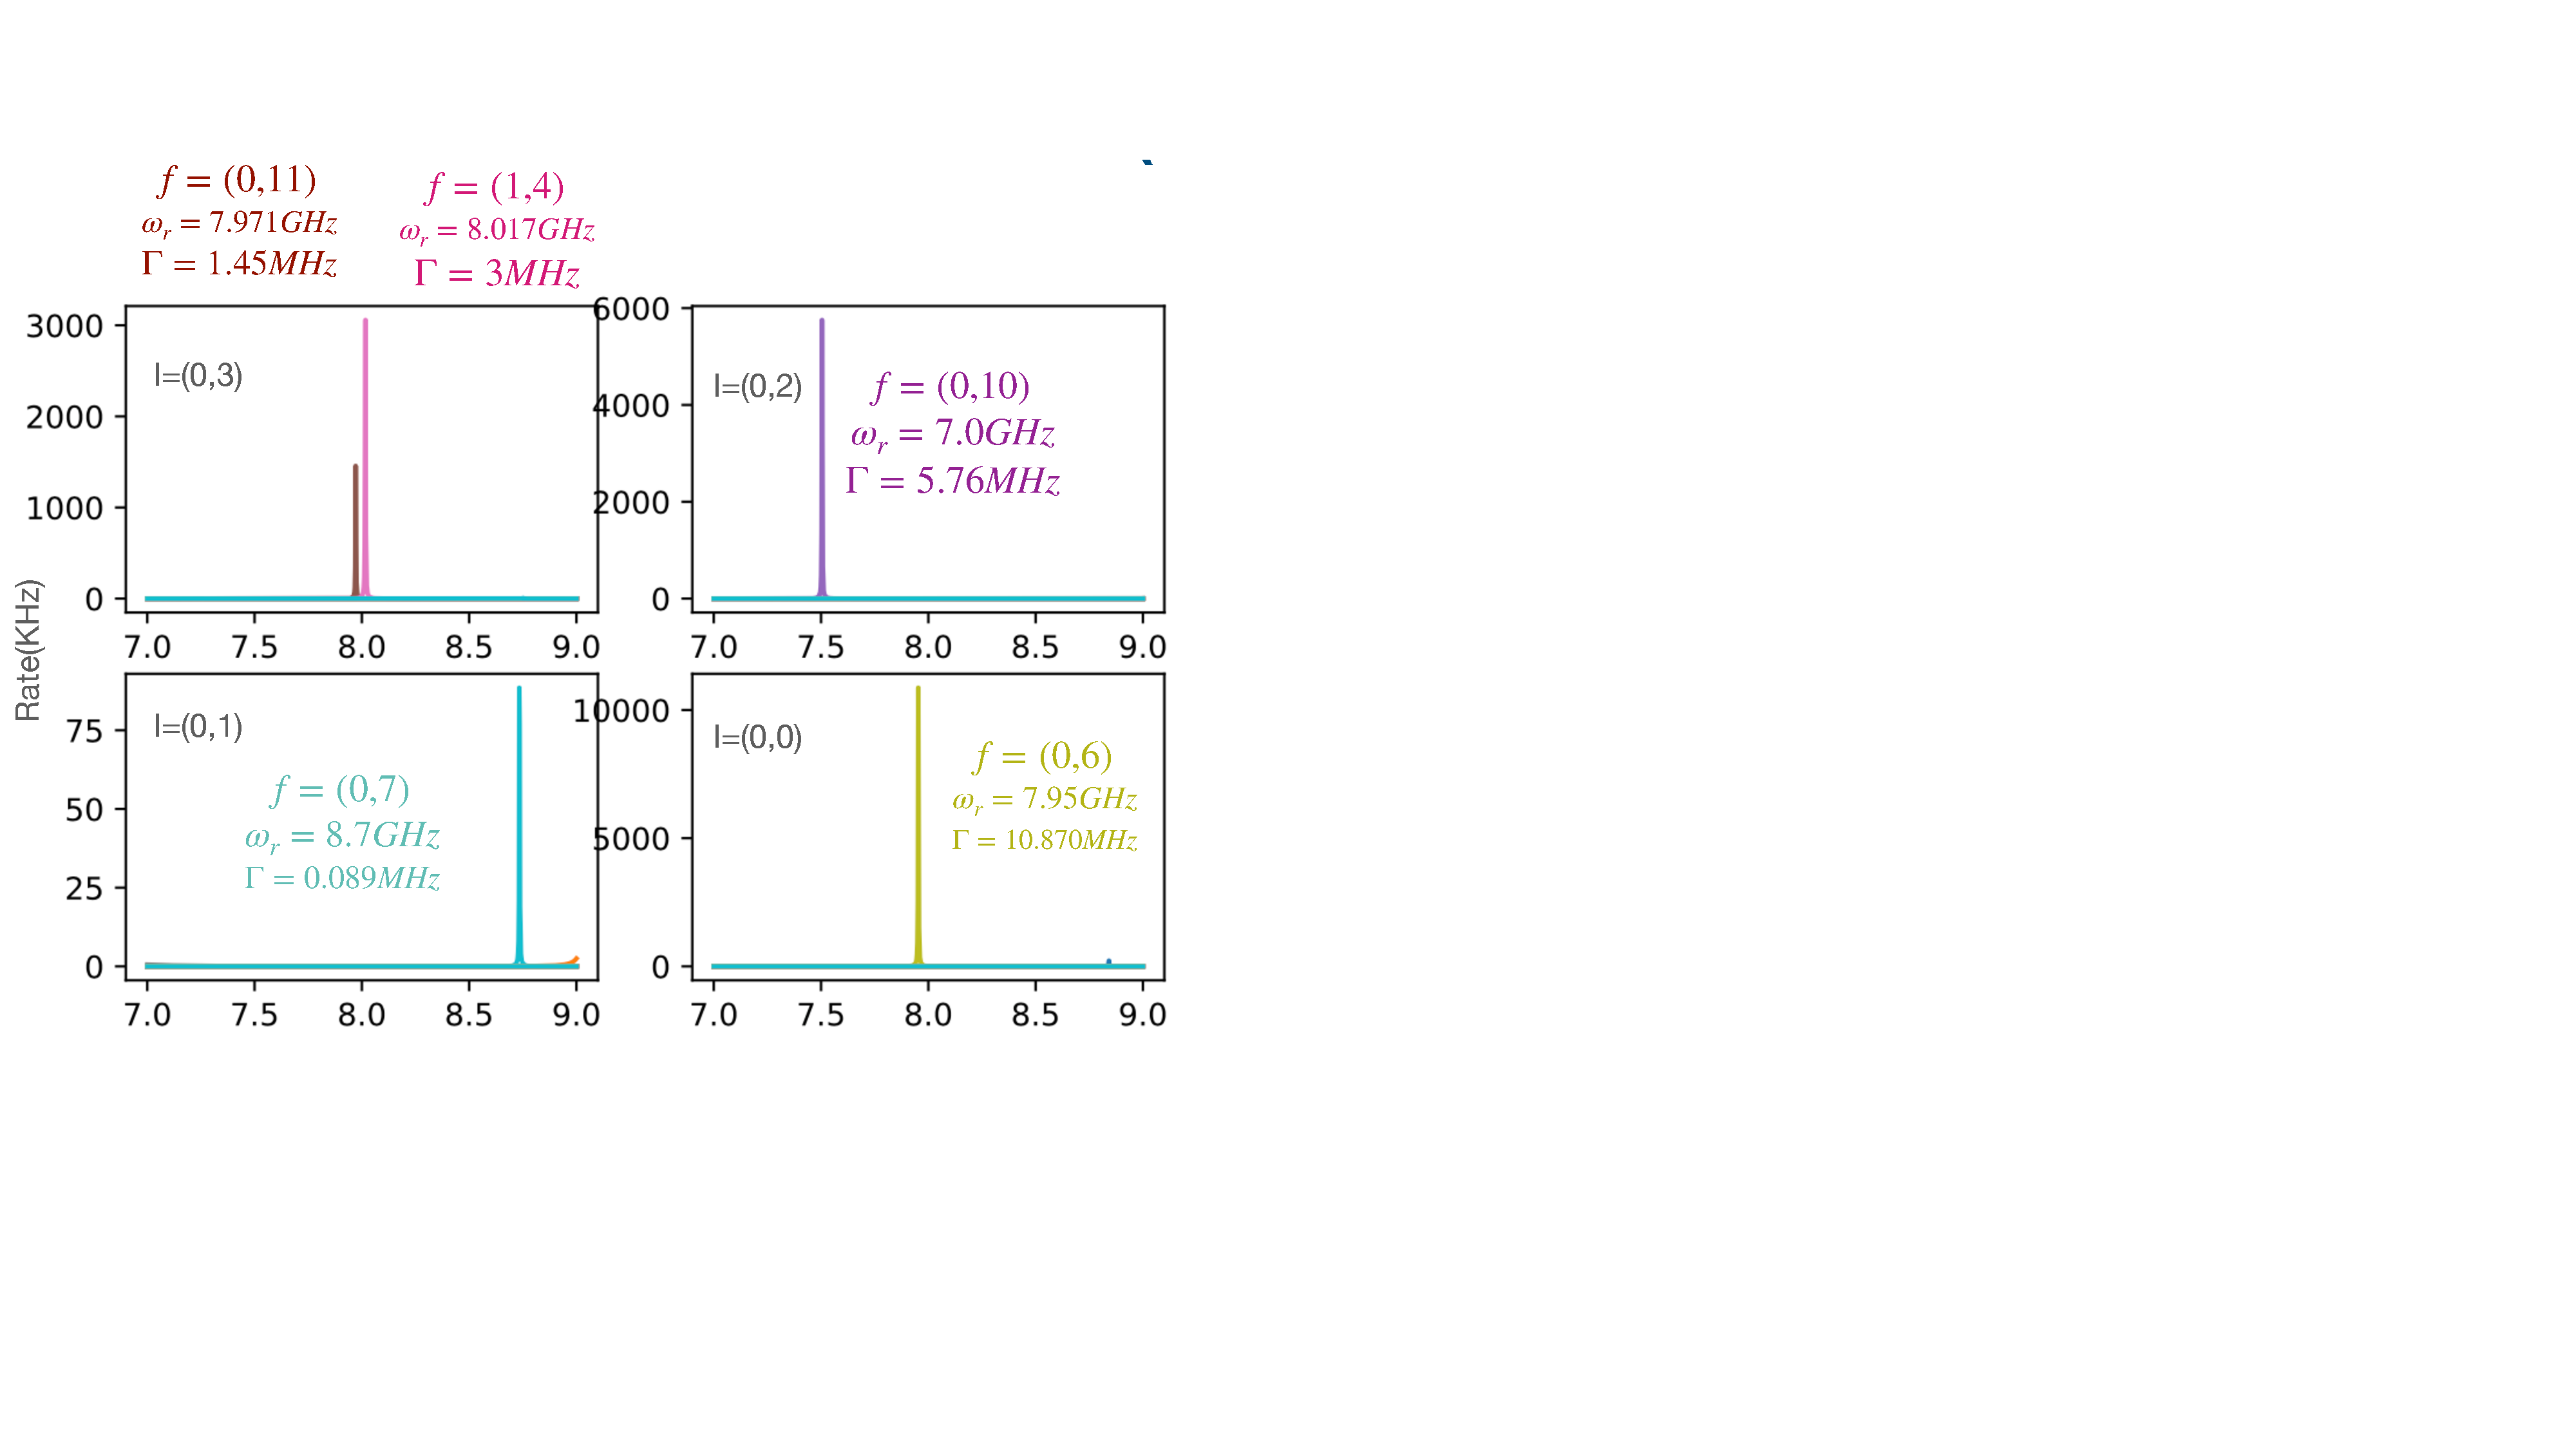
\includegraphics[width=0.5\textwidth]{Figures/FG_02.pdf}
%    \caption{Transition rates with FG}
%    \label{fig:FG1}
%\end{figure}
%\begin{figure}[htb]
%    \centering
%    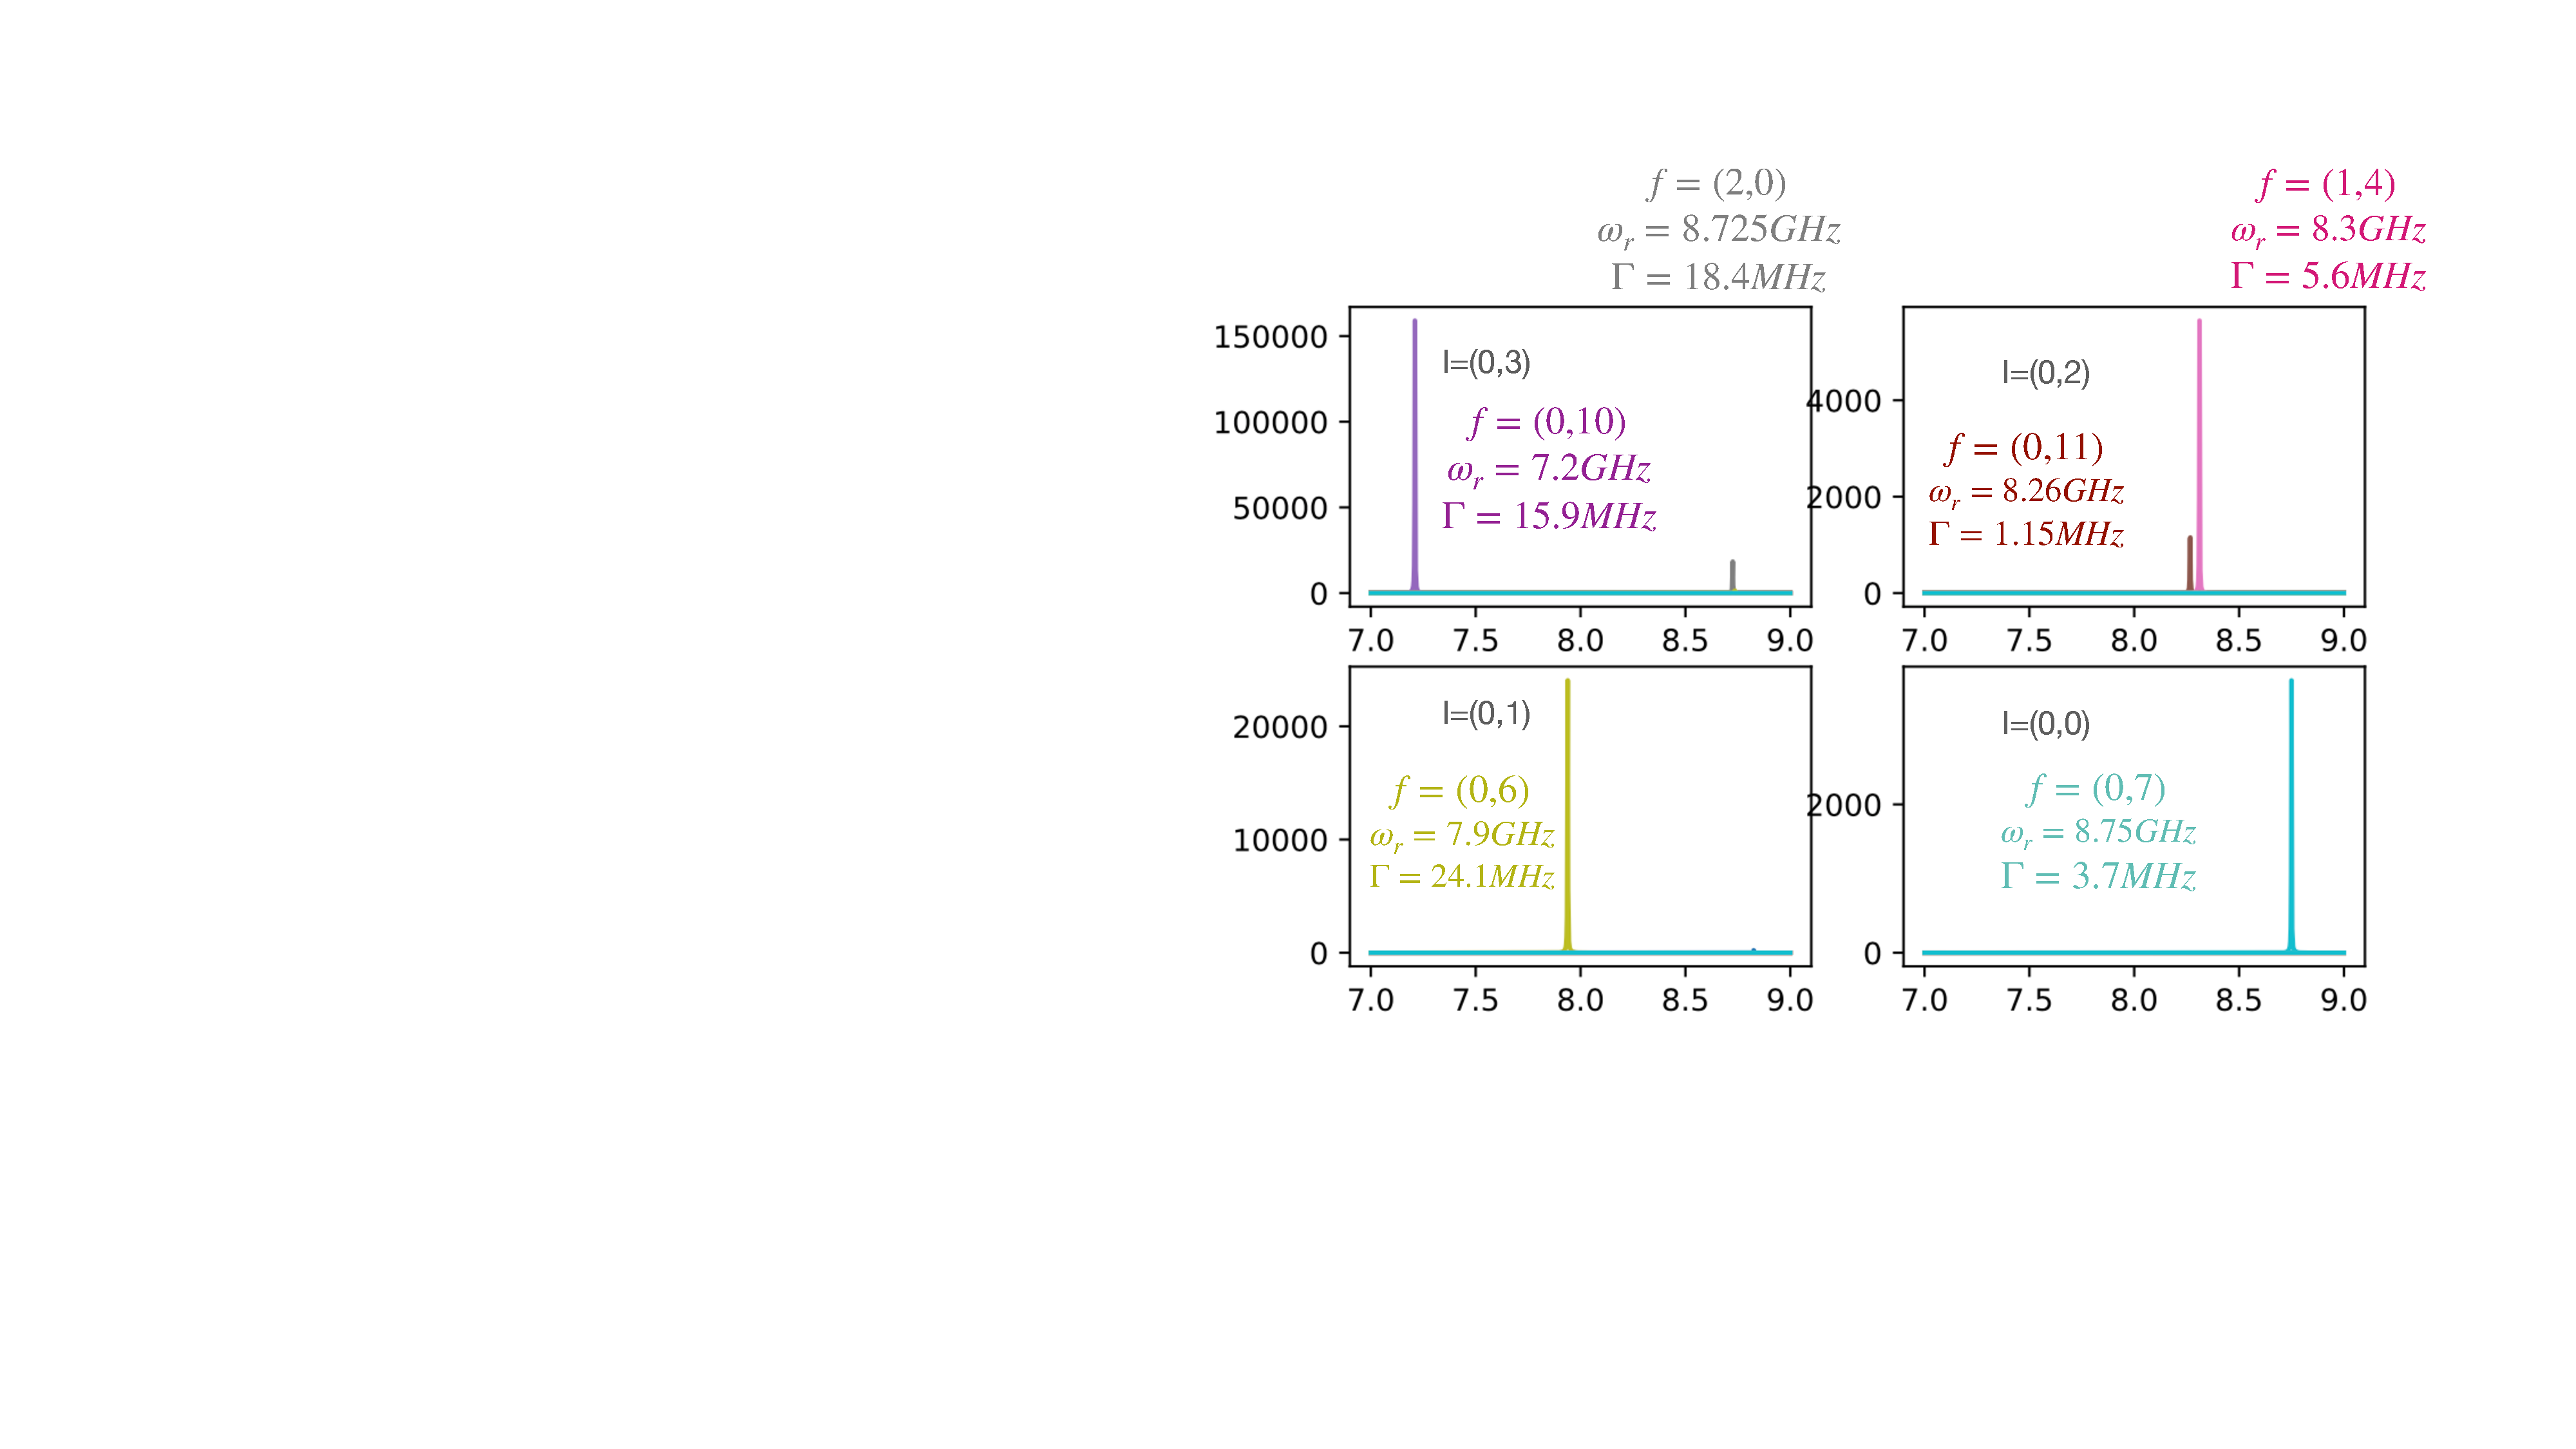
\includegraphics[width=0.5\textwidth]{Figures/FG_01.pdf}
%    \caption{Two-photon process. First-order FG calculations}
%    \label{fig:FG2}
%\end{figure}

\subsection{Transition Rates and Quasienergies}\label{app:Floquet-trans}
Below we guess process responsible for each transition using first and second order fermi's golden rule calculations. We have computed rates using fermi's golden rule up to second order terms, as many of these transitions occur between a parity-conserving states, a forbidden first order transition. We compute these transitions involving up to $4$ readout photons, as suggested by energy conservation. 
Under the same classical approximation, we can identify our parent Hamiltonian as $H_0$ and perturbation $V$ as follows,
\begin{align}
H_0&=H_{\phi}+\omega_\mu \hat a_\mu^\dagger \hat a_\mu+g_{\phi,\mu}\hat N_\phi \hat N_\mu\\
V&=2\sqrt{\bar n_r}(g_{r,\phi} \hat N_\phi+g_{r,\mu}\hat N_\mu)\sin{\omega_d t},
\end{align}
where$\mu$ is the density of states which will be a Dirac Delta function in the absence of loss while it will be Lorentzian in the presence of loss $\frac{\kappa}{2\pi}=50$. In units of $\hbar$ we have,
\begin{align}
    \Gamma_{i\rightarrow f}&=|\braket{f|H_1|i}|^2\mu(E_i-E_f)\quad\textrm{(first-order)}\\
&=\sum_m\frac{|\braket{f|H_1|m}\braket{m|H_1|i}|^2}{|E_i-E_m-k\hbar\omega_d|^2}\mu(E_f-E_i-n\hbar \omega_d)\nonumber\\&\quad\quad\quad\textrm{(second-order)}
\end{align}
We use a Lorentzian density of states at a $\frac{\kappa}{2\pi}=1.5 \ \mathrm{KHz}$. Here $k<n$ is used to compute the detuning with the intermediate state involved in the transition. Note that increasing the width of the Lorentzian $\kappa$ resulting in an increase in the FG rates. Thus, here the decay rate does not yield any insights into the diabaticity at the transition, and hence the $\kappa$ variation here is not the same as the $\kappa$ variation in Sec.~\ref{sec:LZ}.

While these calculations include stark shifts in the energies of the states, we know that the first-order perturbative correction is not enough for some of the more higher states as seen in the comparisons of quasi-energies from Floquet simulations and predicitions of stark shifted transitions. Thus, the computation below is only based on a heuristic developed from this approximate calculation. All transitions are computed at $\bar n_r=50$. We note that the fermi's golden rule calculations higher rates at the frequencies predicted by $g_{\phi\mu}=0$ case where the two frequencies are extremely different, for example, transitions $10$ and $14$. This happens since the Fermi's golden rule calculations are only approximately computing the stark-shifted energies for states which are more hybridized due to the presence of coupling $g_{\phi\mu}$. This behaviour is evident in Figs.~\ref{fig:Trans0},~\ref{fig:Trans1},~\ref{fig:Trans2}. We will compare the considerable FG rates with well-separated quasi-energy gap at the avoided crossings  $\Delta_{ac}$ seen in these figures.

For the case of $\ket{i}=\ket{\tilde{0},\tilde{0}}$ shown in Fig.~\ref{fig:Trans0}, we quote the rates for each process and state how many readout photons were involved, guess the possible intermediate state and whether it could be a first- or second-order process. This heuristic analysis is still interesting since it helps us understand the processes involved behind general MIST processes and p-MIST processes, identifying any unique feature or extremely high rates, if so. 
\begin{itemize}
    \item[1] This is a first order transition involving three readout photons $(3r)$ which yields a fermi's golden rule rate of $40 \ \mathrm{KHz}$. 
    \item[2] The first process is a second-order process which absorbs two photons $(2r)$ through an intermediate state with energy close to $E_i+\omega_r$ at a rate of $4 \ \mathrm{MHz}$ where $\Delta_{ac}=4 \ \mathrm{MHz}$. The second process is a second-order which absorbs four photons $(4r)$ through an intermediate state close to $E_i+3\omega_r$ at a rate of $22 \ \mathrm{KHz}$. 
    \item[3] This is a Rabi transition involving a virtual state via a second-order two-photon process $(2r)$ at a rate of $0.028 KHz$. 
    \item[4-6] The first transition is a second order two-photon process $2r$ with an FG rate of $1.26 \ \mathrm{KHz}$ at $\omega_r=9.36 \ \mathrm{GHz}$. The second process is a Rabi transition at a rate of $10 \ \mathrm{KHz}$. 
\end{itemize} 
\begin{figure*}
    \centering
    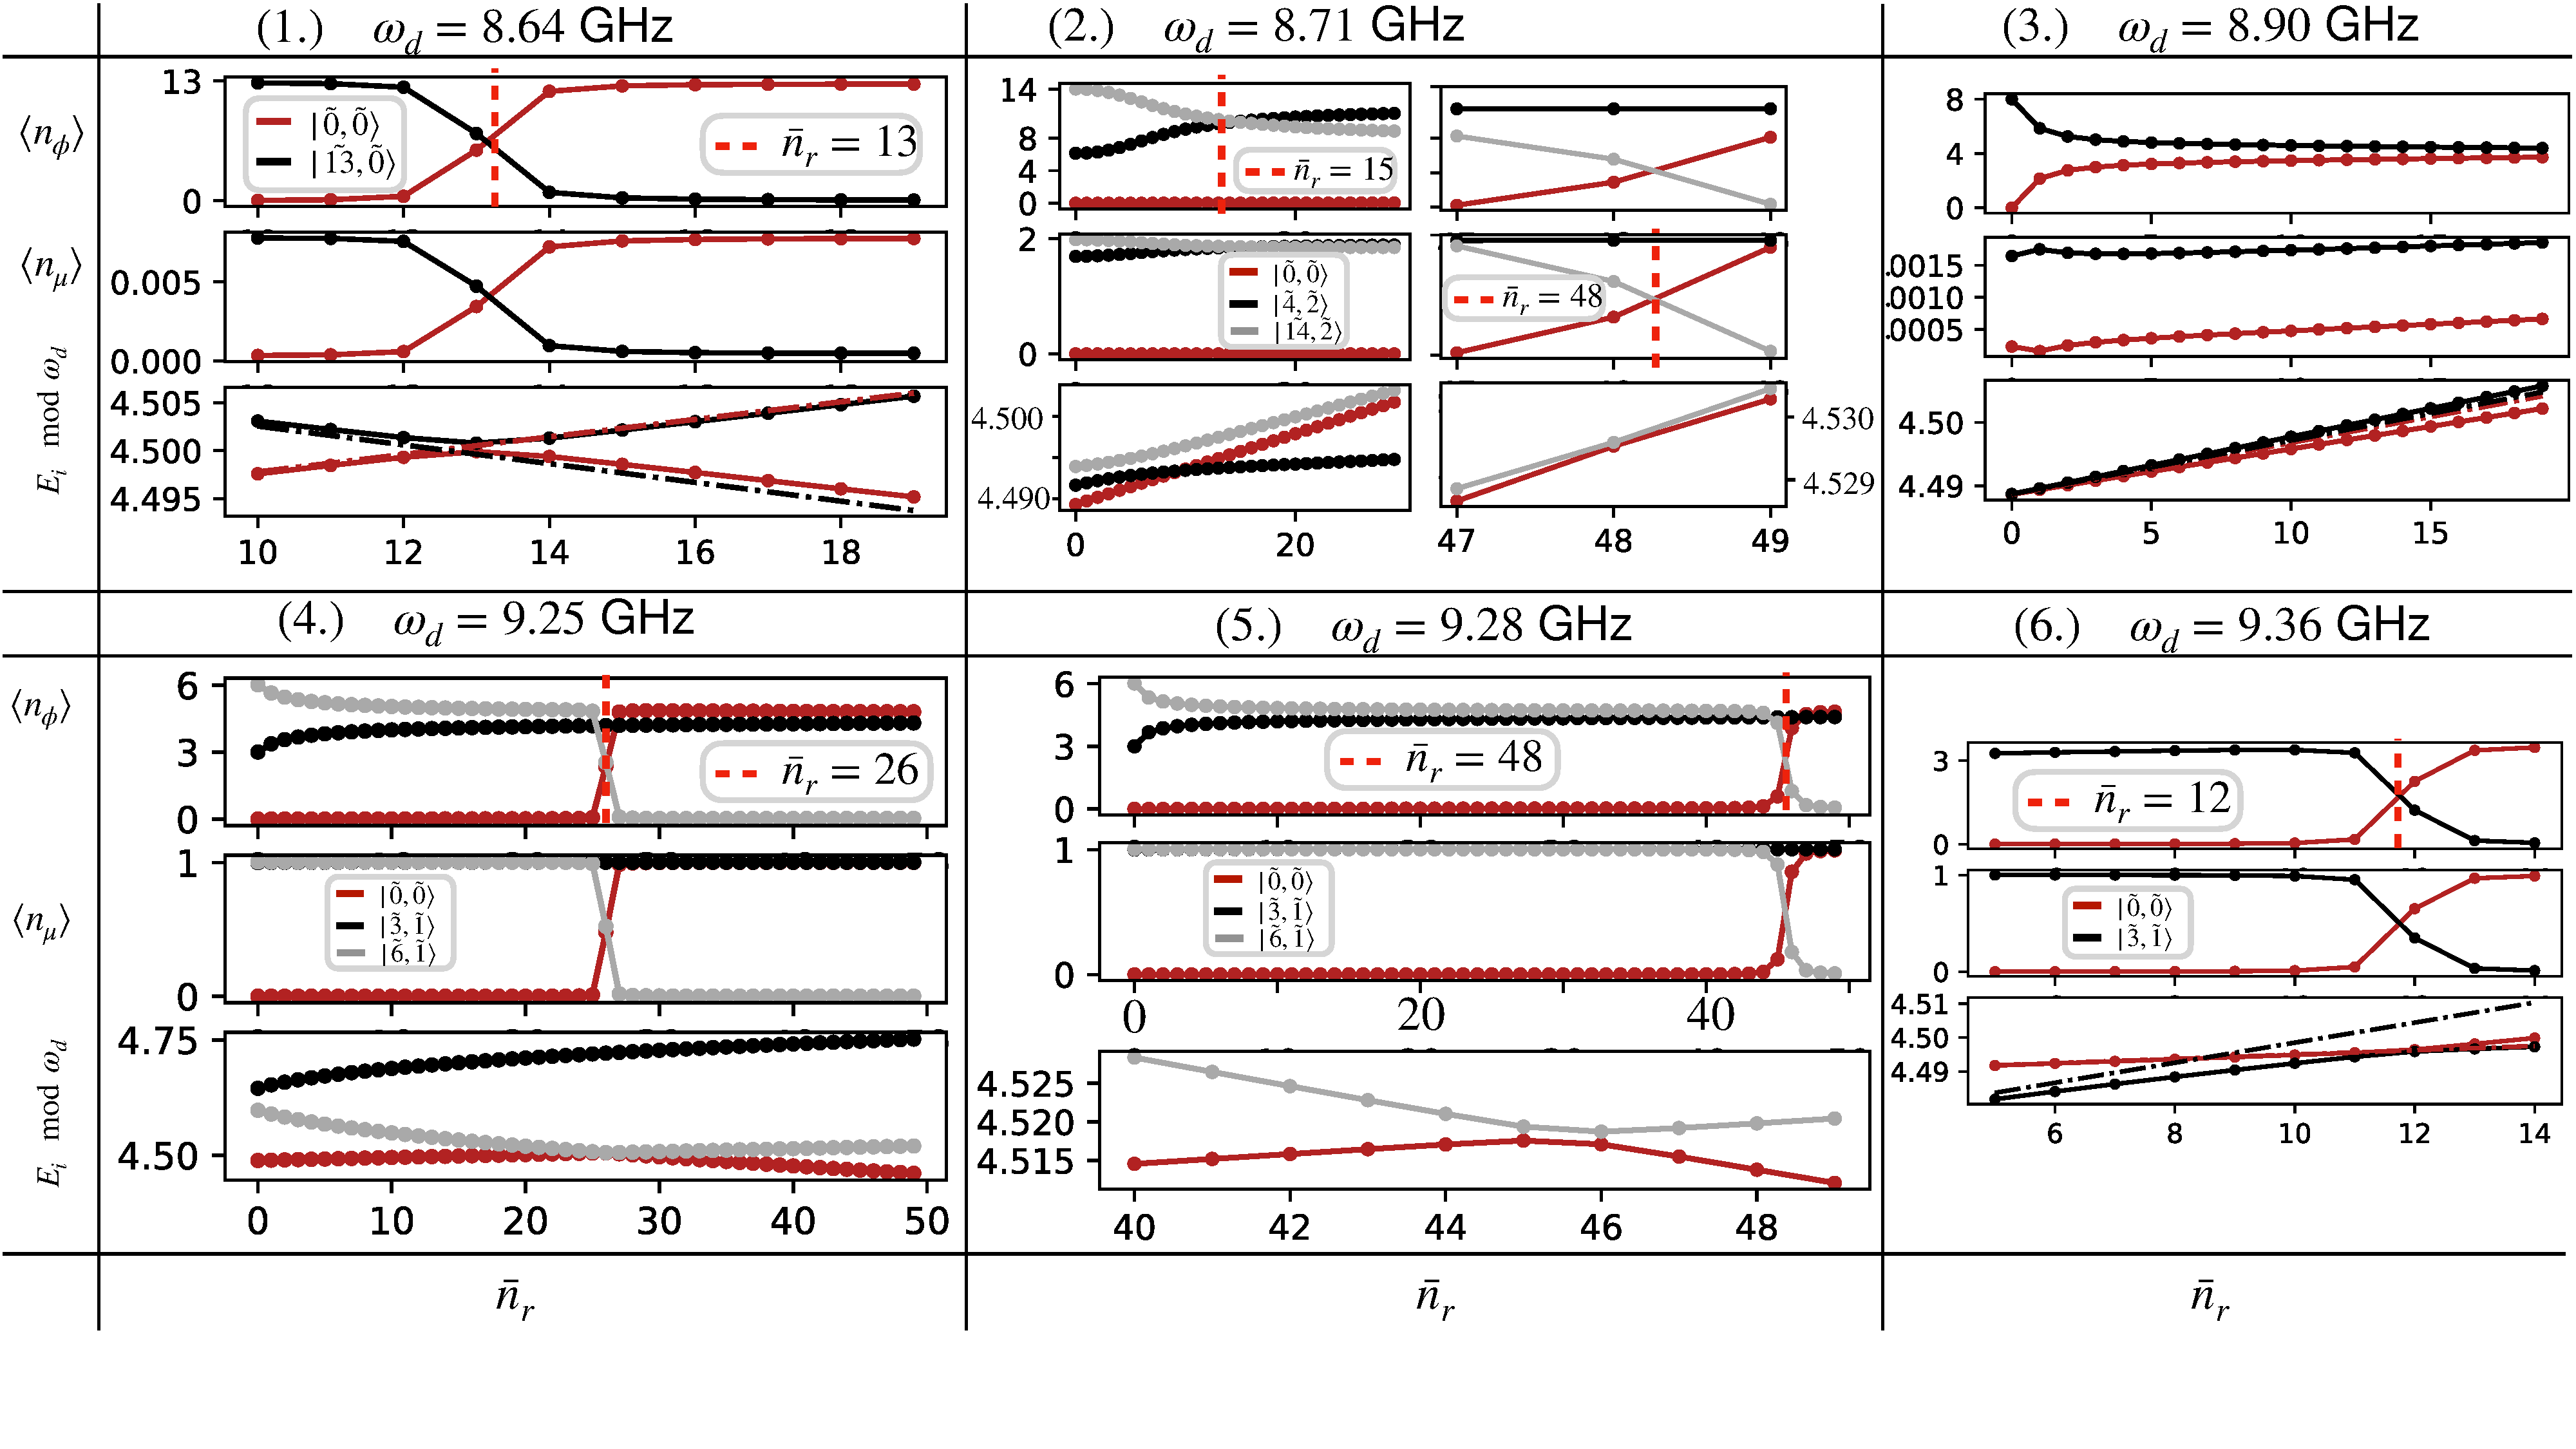
\includegraphics[width=1.0\textwidth]{Figures/Trans0.pdf}
    \caption{MIST processes from Table~\ref{tab:p-MIST} involving the $\ket{\tilde{0},\tilde{0}}$ state. (Top row) Fluxonium subspace $\braket{n_\phi}$. (Middle) Parasitic mode subspace $\braket{n_\mu}$ (Bottom) Stark-shifted eigen-energies (dashed) and quasi-energies (solid) from Floquet simulations, corresponding to the initial state $i$ as per the legend. Inset shows avoided crossing of quasi-energies. Floquet results are extracted from numerical data used for Fig.~\ref{fig:Floquet}.}
    \label{fig:Trans0}
\end{figure*}
Next, we look at the transition rates for the $\ket{\tilde{0},\tilde{1}}$, the state involved in the computation as well as readout in a low-frequency fluxonium, shown in Fig.~\ref{fig:Trans1}.
\begin{itemize}
    \item[7] This is a second order process involving four readout photons $(4r)$ at a rate of $21 \ \mathrm{KHz}$. The intermediate state involved is close to a frequency of $E_i+3\omega_r$.
    \item[8] This is a second order process involving two readout photons $(2r)$ with a transition rate of $45 \ \mathrm{KHz}$. The energy gap at the avoided crossing for this transition is less than $1 \ \mathrm{MHz}$. 
    \item[9] This is a second order process involving four readout $4r$ photons occurring at a rate of $0.95 \ \mathrm{KHz}$, where the intermediate state energy is close to $E_i+3\omega_r$. 
    \item[10] This is a second order process involving two readout $2r$ photons occurring at a rate of $91 \ \mathrm{KHz}$. Fig.~\ref{fig:LZ} also confirms that the transition 9 occurs with a higher probability compared to transition 8. The energy gap at the avoided crossing is
    \item[11] This is a first order process involving three readout photons $(3r)$ occurring at a rate of $2.2 \ \mathrm{KHz}$. 
    \item[12] This is a second order process involving two readout photons $(2r)$ occurring at a rate of $52 \ \mathrm{KHz}$ where $\Delta_{ac}=1.1 \ \mathrm{MHz}$.
\end{itemize}
\begin{figure*}
    \centering
    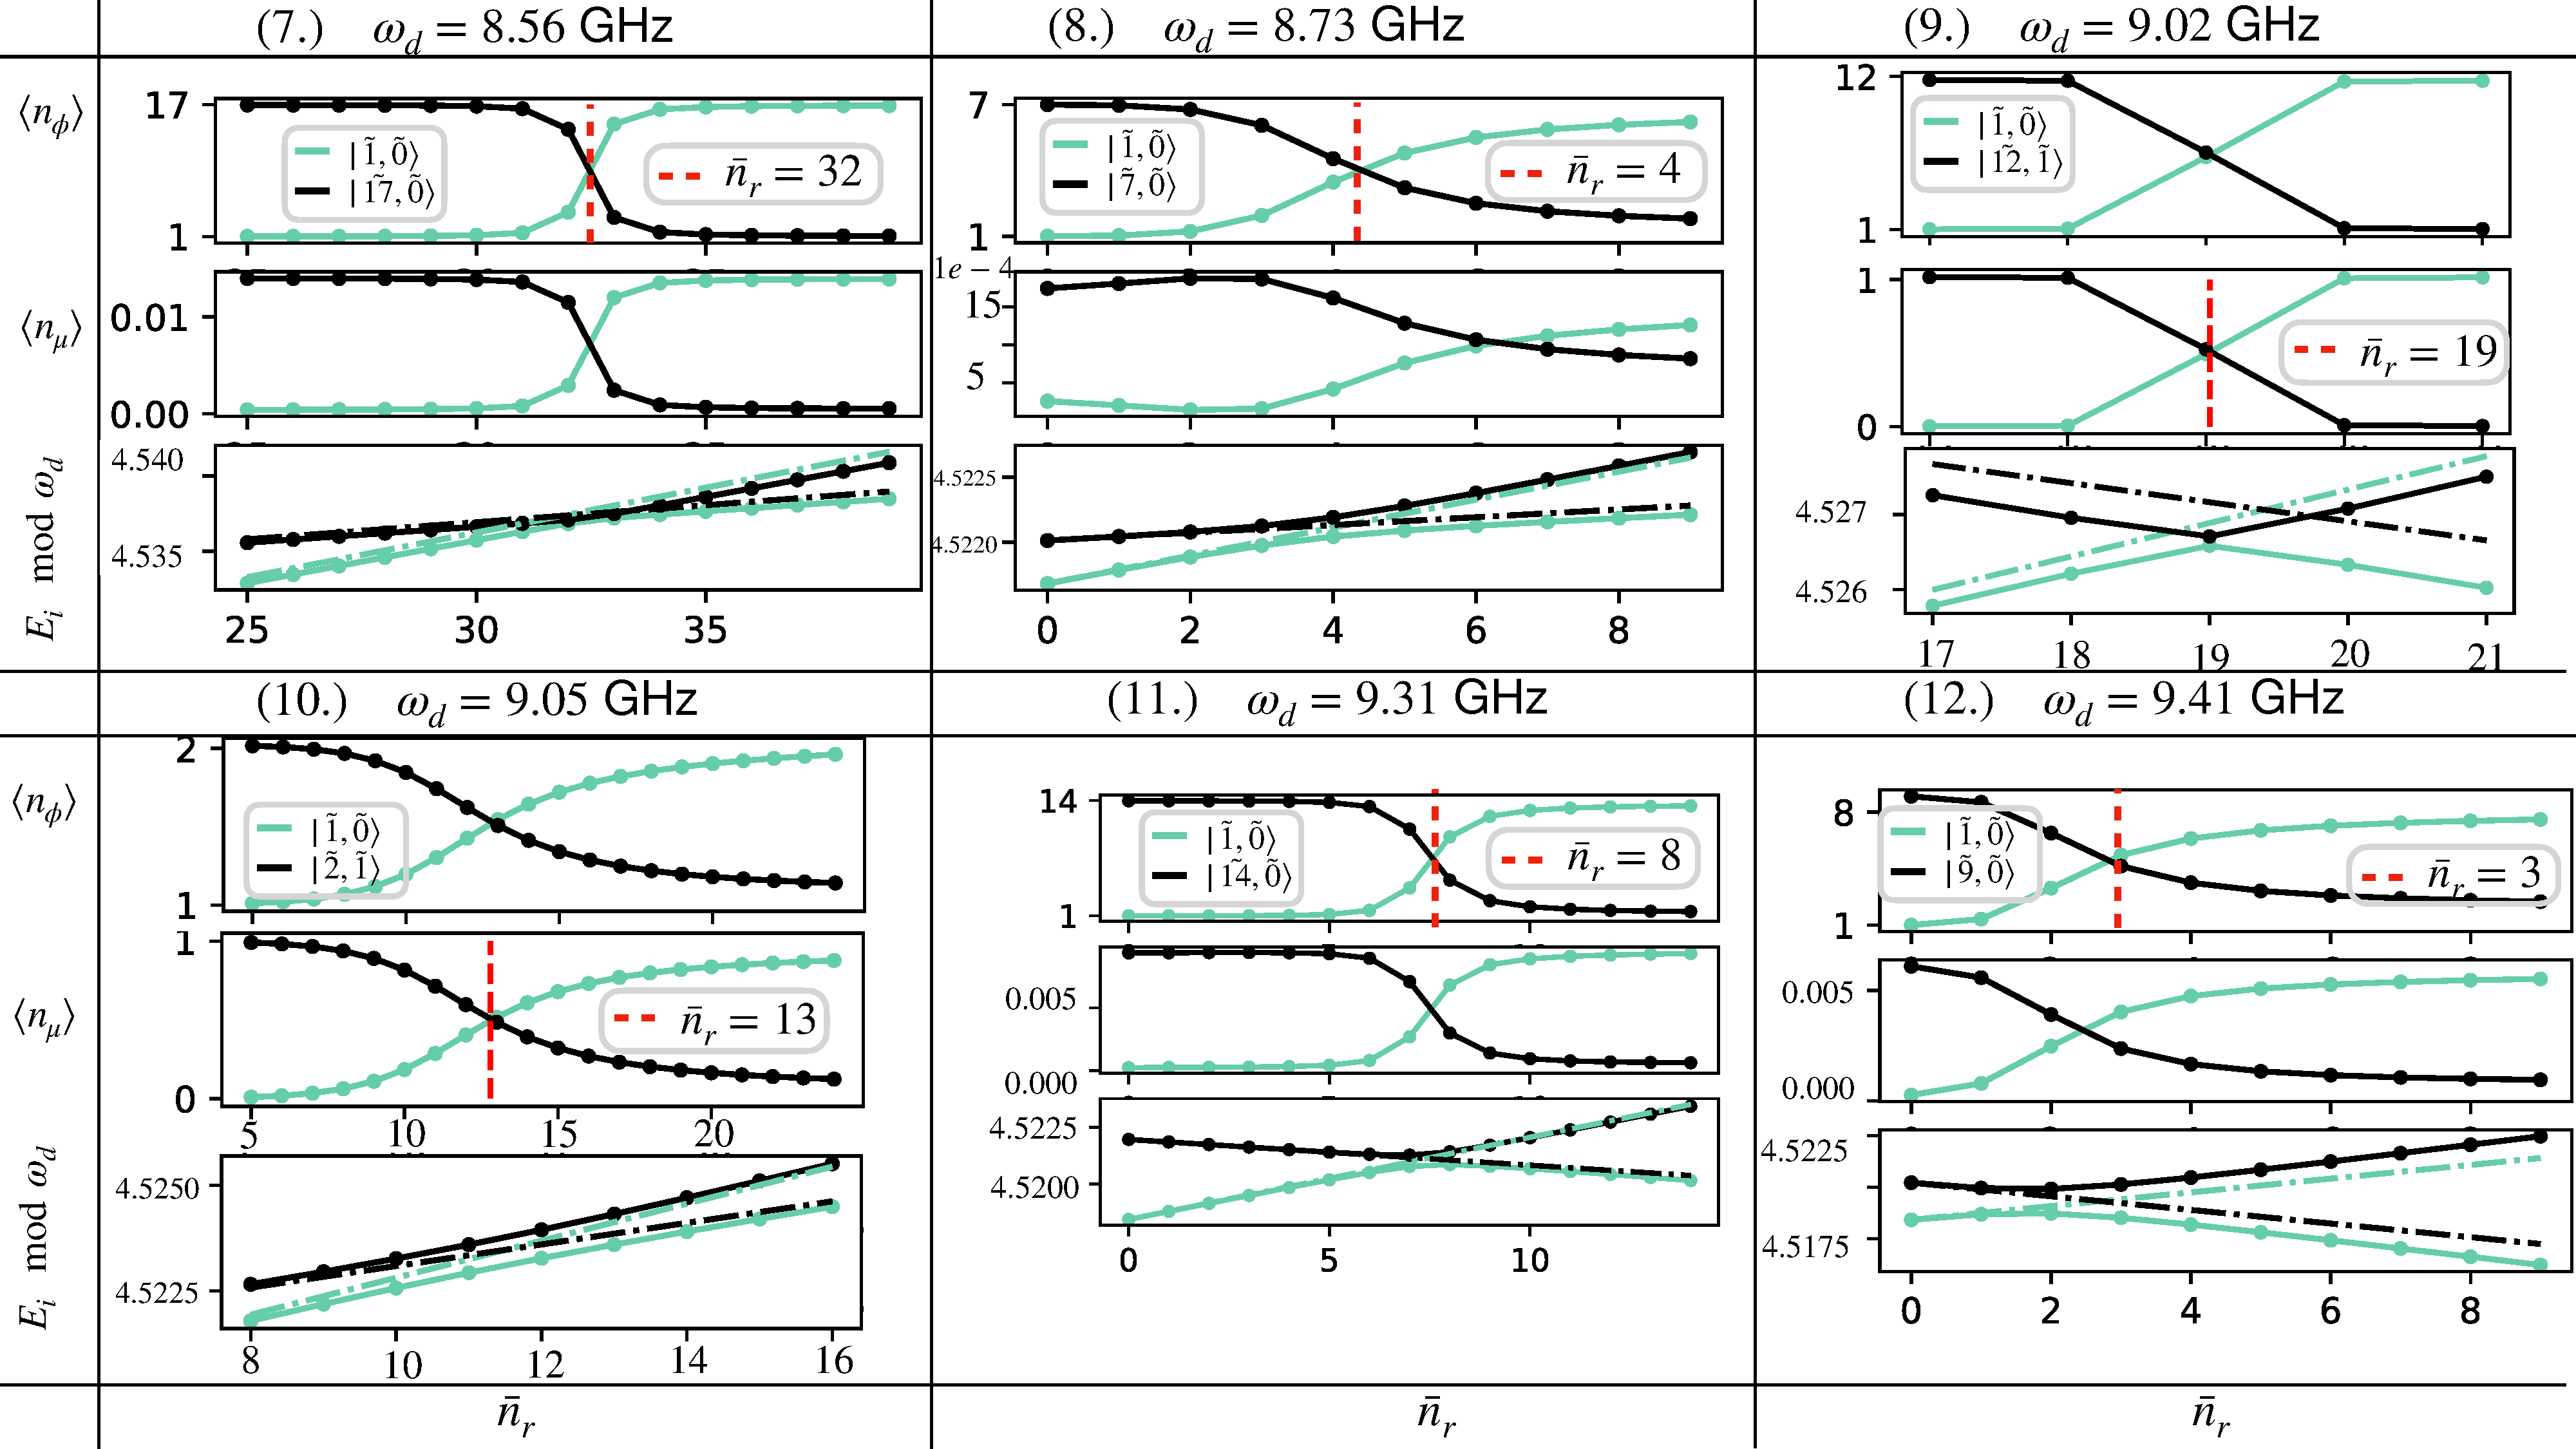
\includegraphics[width=1.0\textwidth]{Figures/Trans1.pdf}
    \caption{MIST processes from Table~\ref{tab:p-MIST} involving the $\ket{\tilde{1},\tilde{0}}$ state. (Top row) Fluxonium subspace $\braket{n_\phi}$. (Middle) Parasitic mode subspace $\braket{n_\mu}$ (Bottom) Stark-shifted eigen-energies (dashed) and quasi-energies (solid) from Floquet simulations, corresponding to the initial state $i$ as per the legend. Inset shows avoided crossing of quasi-energies. Floquet results are extracted from numerical data used for Fig.~\ref{fig:Floquet}.}
    \label{fig:Trans1}
\end{figure*}
Finally, we look at the transition rates for the $\ket{\tilde{0},\tilde{2}}$, the state involved in the readout of a low-frequency fluxonium, shown in Fig.~\ref{fig:Trans2}.
\begin{itemize}
    \item[13] This is a second order process involving two-readout photons $(2r)$ occurring at a rate of $16$ ($1$) MHz which is the same as $\Delta_{ac}$.
    \item[14] This is a second order process involving two-readout photons $(2r)$ occurring at a rate of $2.2 \ \mathrm{KHz}$.
    \item[15] The first process is first order while the second process is second order, both involving $(1r)$ and $(2r)$ readout photons. The rates of these transitions are $1.48 \ \mathrm{KHz}$ and $28 \ \mathrm{KHz}$, respectively. The energy gap at this avoided crossing is $4 \ \mathrm{MHz}$. Thus, this transition appears to be a either a higher order process or a weaker transition.
\end{itemize}
\begin{figure*}
    \centering
    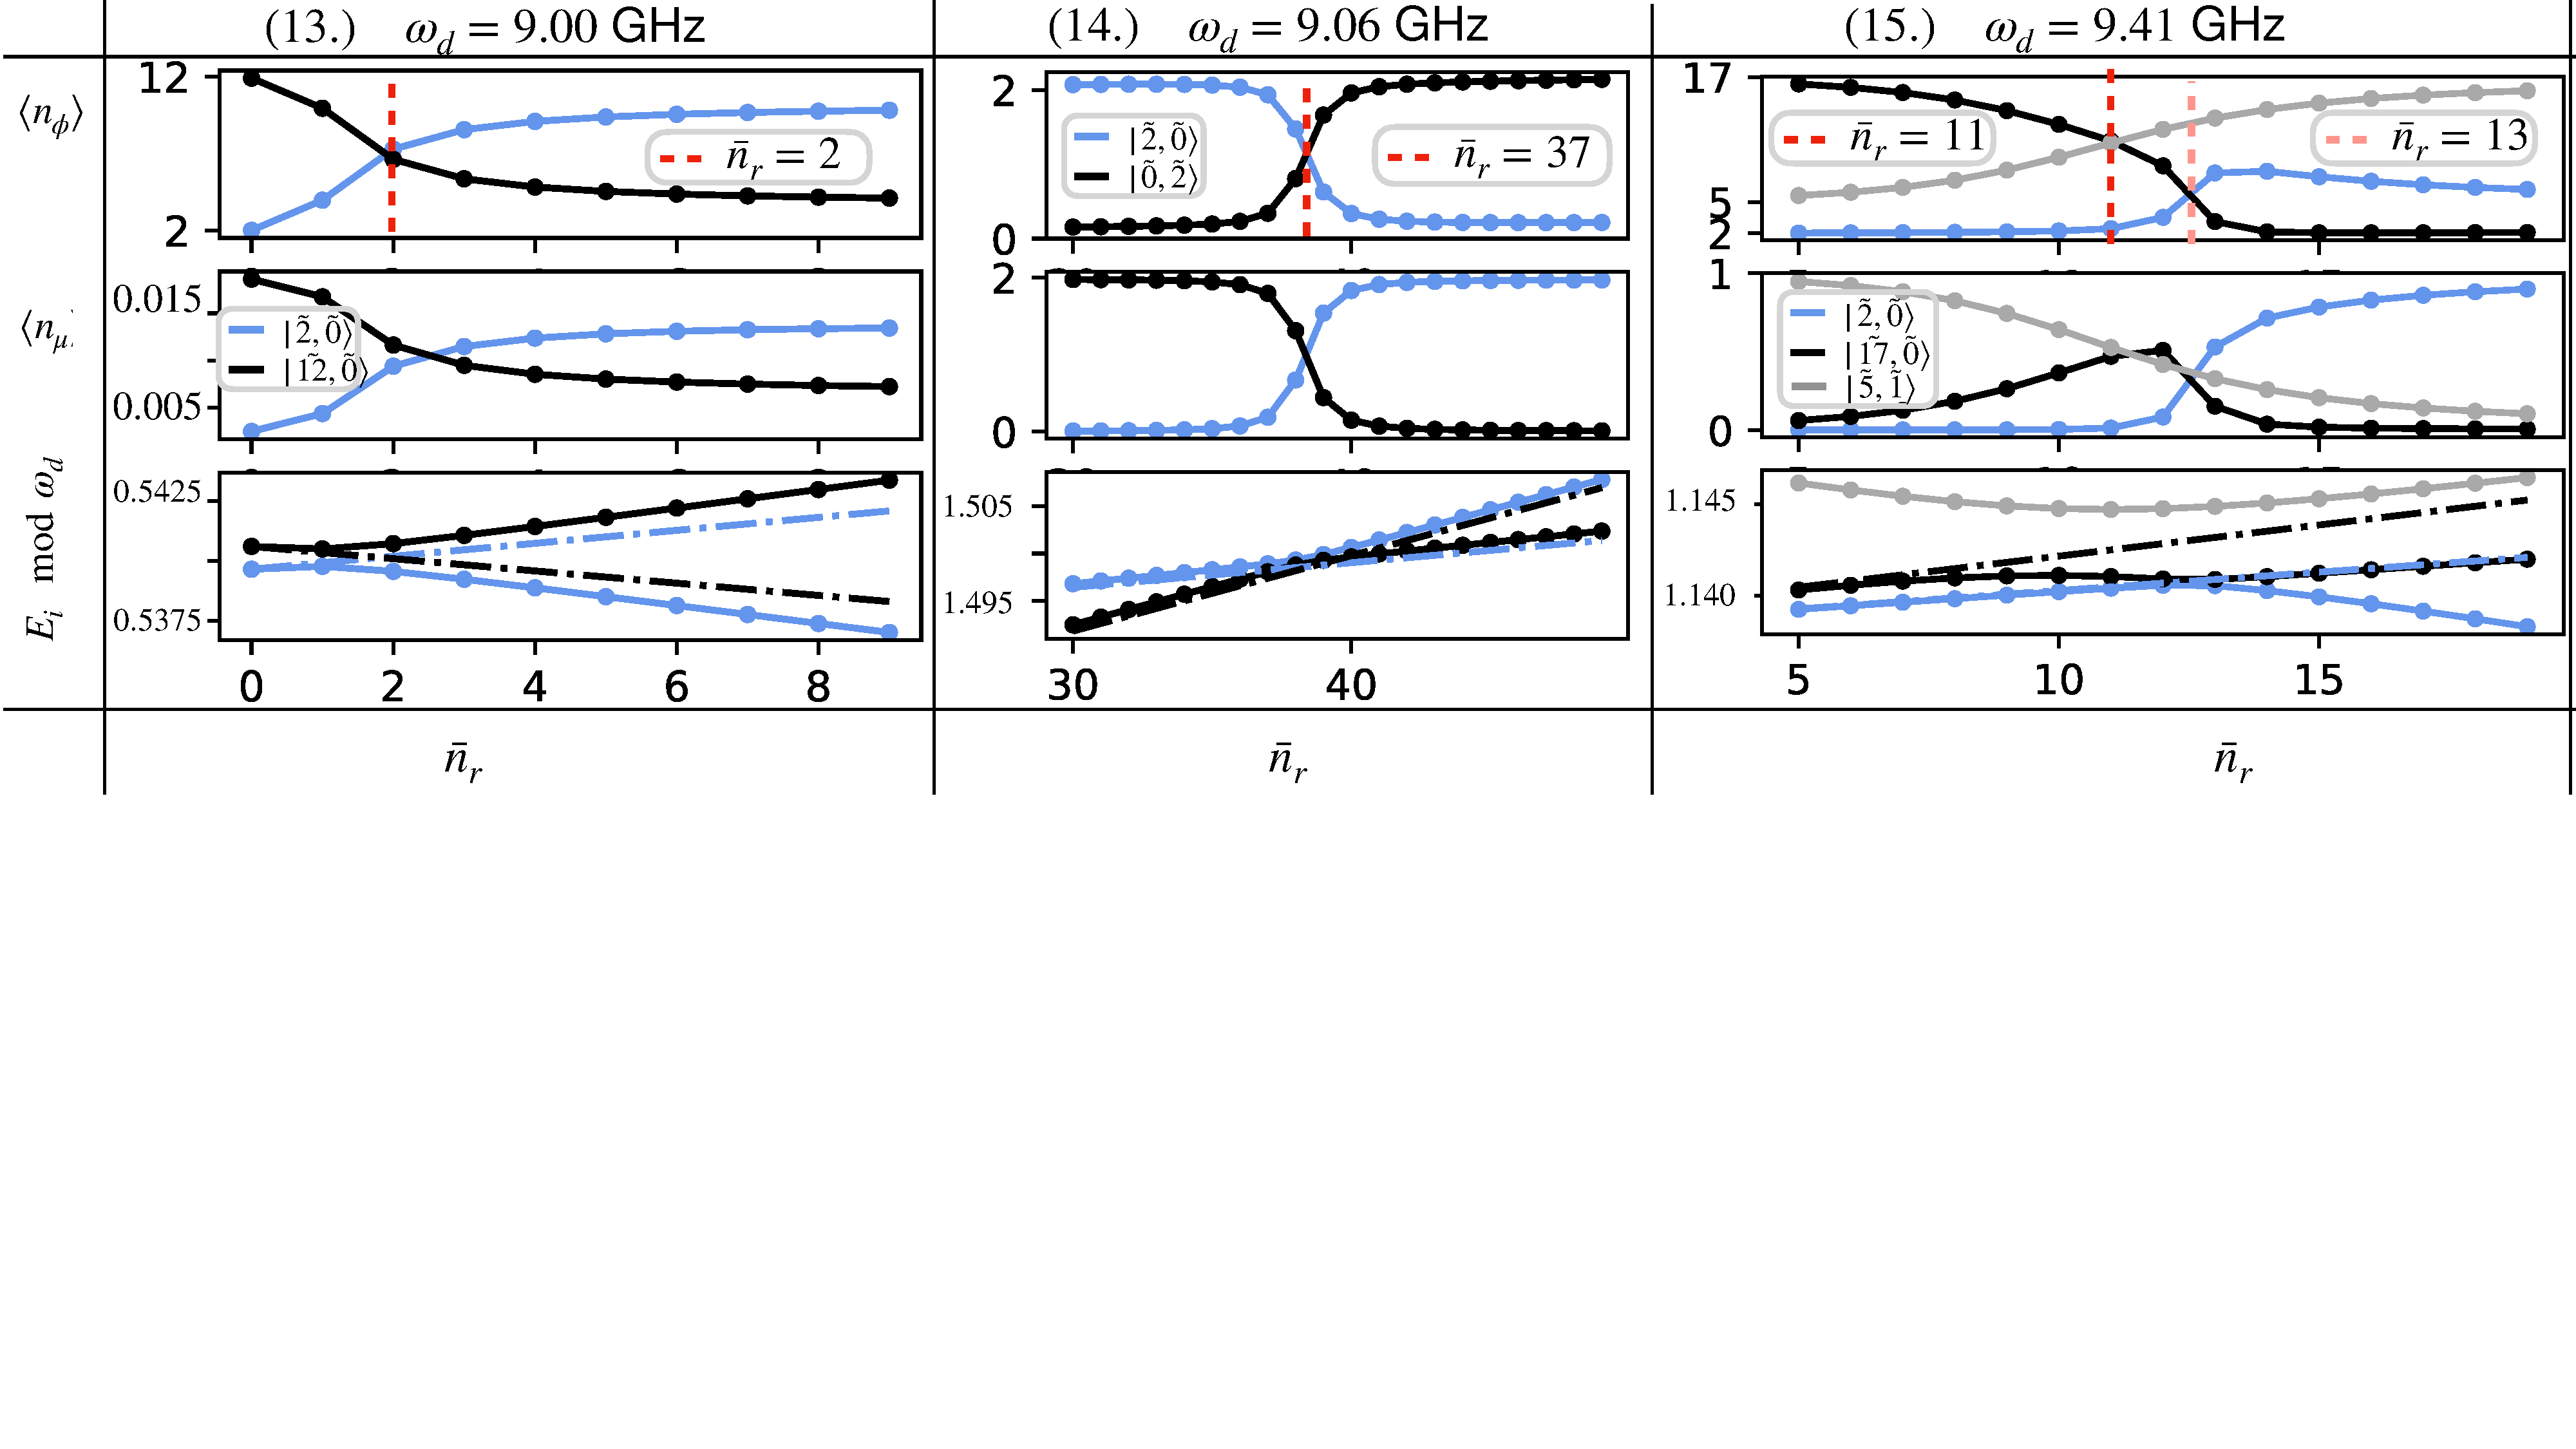
\includegraphics[width=1.0\textwidth]{Figures/Trans2.pdf}
    \caption{MIST processes from Table~\ref{tab:p-MIST} involving the $\ket{\tilde{2},\tilde{0}}$ state. (Top row) Fluxonium subspace $\braket{n_\phi}$. (Middle) Parasitic mode subspace $\braket{n_\mu}$ (Bottom) Stark-shifted eigen-energies (dashed) and quasi-energies (solid) from Floquet simulations, corresponding to the initial state $i$ as per the legend. Inset shows avoided crossing of quasi-energies. Floquet results are extracted from numerical data used for Fig.~\ref{fig:Floquet}.}
    \label{fig:Trans2}
\end{figure*}
\subsection{Landau-Zener Probabilities}\label{app:LZ}
We compute the Landau-Zener probabilties numerically using the quasienergies from the Floquet simulations and analytically using the stark-shifted eigen-energies. In order to convert the Floquet simulation used with variation in $\bar n_r$ at a fixed time $t$ (ignoring the short scale fast dynamics over a time period), in this case, we will use a time-dependent case where $\bar n_r$ varies as $\bar n_r=50(1-e^{-\kappa T/2})^2$ to emulate change in readout photons from dissipation. The numerical calculations use the probability for Landau-Zener transitions given in~\cite{ikeda2022floquet} for an avoided crossing observed between states $i,f$ ,
\begin{align}
    P_{LZ}&=\exp{\Big[-\pi \frac{\Delta_{ac}^2}{2v}\Big]},\\
    \text{where } v&=\sqrt{2\Delta_{ac}\Big|\frac{d^2\epsilon_f}{d\bar{n}_r(t)^2}\Big|_{t_{ac}}}\frac{d\bar{n}_r(t)}{dt}|_{t_{ac}}\Big.
\end{align}
Here, the variable $\epsilon_j$ is the numerically computed quasi-energy obtained from Floquet simulations, while $\Delta_{ac}$ refers to the quasi-energy difference at avoided crossing.

For the analytical calculations, we use the well-known formula (with energy in units of GHz), 
\begin{align}
    P_{LZ}&=\exp{\Big[-4\pi^2 \frac{V}{\frac{\partial\omega_{if}}{\partial\bar n_r(t)}\frac{d\bar n_r(t)}{dt}}\Big]},\\
    \text{where}\quad V&=|\braket{i|H_{t}|f}|^2\\
    \omega_{if}&=E_f+\chi_f(\bar n_r(t))-E_i-\chi_i(\bar n_r(t))
\end{align}
Here $\chi_i(\bar n_r(t)), \chi_f(\bar n_r(t))$ are ac stark shifts in the eigen-energies of $i,j$ due to $\bar n_r$ average readout photons. See app.~\ref{app:stark-shift} for the calculation of these quantities.
\subsection{Parasitic Dephasing due to Thermal Effects}\label{app:dephasing}

In this appendix, we lay out in detail our calculations of dephasing induced by the random occupation of the parasitic modes due to thermal effects. We assume a scenario where the circuit is connected to a bath at $0K$ such that thermal photons can be set to $n_{th}=0$. The parasitic mode is randomly populated to some non-zero $\bar n_\mu$ induced by the coupling of the readout with the parasitic mode. Now, at some point this population will go back to $\bar n_\mu=0$ due to the decay of the parasitic modes dominated by the rate $\kappa_\mu=\frac{\omega_\mu}{Q_\mu}$. Here $Q_\mu,\omega_\mu$ are the quality factor and frequency of the parasitic mode. We are set to compute the dephasing due to the fluctuation in this quantity as the parasitic mode decays. We can compute the total decay rate of the parasitic modes as follows~\cite{gambetta2006qubit}, 
\begin{align}
k_\mu&=\kappa_r \frac{g_{\mu,r}^2}{\Delta^2}+\frac{\omega_\mu}{Q_\mu},
\end{align}
where $\Delta$ is the detuning between the parasitic mode frequency and the readout drive frequency. The first terms and second terms depict contributions from Purcell effect due to the readout resonator ($\approx$ Hz) and the quality factor $Q_\mu$ of the parasitic modes ($\approx \ \mathrm{KHz-MHz}$). The second term dominates the expression and will determine the decay rate of the parasitic modes. 
 

In this context, we use the methods described in Ref.~\cite{clerk2007using} to compute the dephasing of a qubit given the initial occupation of the parasitic mode and the strong coupling between the qubit and the parasitic mode. Here, we use the dispersive Hamiltonian (see Eq.~\ref{eq:dispersive}) of qubit-parasitic mode system, without the readout. This assumption on the system is well-suited to cases where measurement has populated the parasitic mode. In the absence of any state transition in the fluxonium circuit, the parasitic mode is populated to $\bar n_\mu=\mathcal{O}(10^{-4})$ as shown in Fig.~\ref{fig:coupling-Floquet}(a) due to the readout-parasitic mode coupling.
\begin{align}
\frac{H}{\hbar}&=\frac{\omega_q}{2}\sigma_z+\sum_{\mu}\Big(\omega_\mu+k_\mu+\chi_{\mu\phi}\sigma_z\Big) a_\mu^\dagger a_\mu,\\
&+\xi_{\mu r}\hat N_\phi\sin{\omega_d t}
\end{align}
where, $\kappa_\mu$ is the lamb shift, $\chi_\mu$ is the stark shift, and $\omega_\mu$ is the frequency of the parasitic mode. The variable $\omega_q$ denotes the qubit frequency i.e. the energy gap between the ground and the first excited state of the qubit potential. We ignore the qubit drive in this case since it will not play a role in the question of concern. In the presence of a qubit coupling, the state transitions will dominate the lifetimes and thus calculation of dephasing rates takes a backseat. In this scenario we are in the weak damping, strong coupling limit as $g_{\mu\phi}$ is of the order of GHz while the damping $\kappa_\mu=\frac{\omega_\mu}{Q_\mu}$ is of the order of MHz or KHz since all parasitic modes are designed to be high $Q$ cavities. In the limit of zero temperature Ref.~\cite{clerk2007using} shows that the dephasing rate coincides with what has been found in Ref.~\cite{gambetta2006qubit}. We use the calculations for the dispersive Hamiltonian (see Eq.~\ref{eq:dispersive} in App.~\ref{app:Hamiltonian}) to calculate for the drive-dependent dephasing rate at zero temperature quoted in~\cite{gambetta2006qubit,clerk2007using} assuming an initial $\bar n_r$.

\begin{align}
    \Gamma_\theta&=\sum_\mu \frac{1}{2}\frac{|\xi_{\mu,r}|^2\chi_{\mu,\phi}^2\kappa_\mu}{[(\Delta+\chi_{\mu,\phi})^2+(\kappa_\mu/2)^2]}\nonumber\\
    &\quad\times\frac{1}{[(\Delta-\chi_{\mu,\phi})^2+(\kappa_\mu/2)^2]}\\
&=\sum_\mu \Big[\frac{\chi_{\mu,\phi}^2\kappa_\mu}{\Delta^2+\kappa^2/4+\chi_{\mu,\phi}^2}\Big]\bar n_\mu,\label{eq:dephasing}
\end{align}

The thermal population of the parasitic modes is capped at $10^{-3}$ for $T=50mK$  (see App.~\ref{app:Hamiltonian}) inducing a dephasing rate of $\Gamma_\phi=10^{-6} \ \mathrm{GHz}$. 
\section{Alternative Circuit}\label{app:alt_circuit1}
\singh{Here goes the details on Will Oliver's parameters and figures for coupling strengths etc.}



\bibliography{refs.bib} 

\end{document}

